\documentclass[11pt,letterpaper]{article}
\usepackage[letterpaper,margin=1in]{geometry}
\usepackage[T1]{fontenc}
\usepackage{url}
\usepackage{microtype}
\setlength{\emergencystretch}{3em}
\usepackage{lmodern}
\usepackage{amsmath,amssymb}
\usepackage{booktabs}
\usepackage{graphicx}
\usepackage[round,authoryear]{natbib}
\usepackage[colorlinks=true,linkcolor=blue,citecolor=blue,urlcolor=blue]{hyperref}
\newtheorem{proposition}{Proposition}[section]
\DeclareRobustCommand{\Propref}{\ref{prop:bound}}
% Preprint build, DERIVED from paper.tex by scripts/make_preprint_version.py.
% Do not edit this file: edit paper.tex and re-run the generator.

\title{Differentiable Barnes--Hut Gravity: A Provable Second-Derivative Error Bound,
  and Its Validation at 16.7 Million Particles}
\author{Yuchen Wang\\[4pt]
\normalsize Department of Computer Science and Technology, Tsinghua University, Beijing 100084, China\\[2pt]
\normalsize \texttt{yagamilight0620@qq.com}
\and Xin Wang\\[4pt]
\normalsize Xiamen Xiangyu Group Co., Ltd., Xiamen 361000, Fujian, China}
\setlength{\emergencystretch}{3em}
\date{\today}
\begin{document}
\maketitle
\begin{abstract}
Gradient-based inference differentiates the force, so what enters a vector--Jacobian product is the
potential's second derivative --- the tidal tensor --- yet every published remainder for tree and
fast-multipole operators bounds the potential or the force. We derive the missing statement: a
per-interaction remainder bound for the second derivative of a truncated multipole expansion,
Dehnen-shaped but one derivative higher, with exact rather than fitted per-order constants and
explicit dependence on the multipole order, the size-to-distance ratio, and the cell's mass
distribution. We implement it in Laniakea-HMMP, a differentiable Barnes--Hut operator whose
acceptance criterion the same remainder bounds (Proposition~\ref{prop:bound}).

The bound is verified rather than assumed. It holds with no violation on controlled single cells, where
it is $11$--$48\times$ loose, on the $1.64$M far interactions the real CAMELS snapshot actually admits
at $2.3$M particles (median looseness $426\times$), and on the full $16.7$M-particle snapshot (median
$436\times$). It is controlled by the distance from the centre of mass to the farthest particle, not by
the cell's geometric size, so a size-based opening test at fixed $\theta$ is not a fixed error bound.

What is missing is a bound, not a better statistic: the worst query node is $10$--$35\times$ worse than
the mean, and self-certification from the operator's own next-order surplus understates the worst-node
error by five orders of magnitude across four tree sizes and $30$ seed-runs. We validate the complete
operator against the exact force \emph{and} its Jacobian out to $16.7$M particles on sampled query
nodes, and measure the
adjoint a reconstruction actually descends on: it contracts the per-node errors rather than amplifying
them. Every accuracy result is post-correction of a disclosed octree defect, which bought
$11$--$33\times$ at no cost.
\end{abstract}
\noindent\textbf{Keywords:} gravitation --- N-body simulations --- computational astronomy --- dark matter --- large-scale structure of the universe
\vspace{1.5em}
\section{Introduction}
Simulating gravitational dynamics at cosmological scale is an exascale N-body problem: the
pairwise force sum is $O(N^2)$, and at $N\sim10^6$--$10^7$ particles that sum dominates the cost
of every time step. The Barnes--Hut tree \citep{barnes1986} and the fast multipole method
\citep{greengard1987} solve the cost problem by replacing distant pairwise interactions with a
truncated multipole expansion. They are the workhorses of production cosmology codes, but they are
written as hand-tuned numerical kernels, they are not differentiable, and the error they incur is
controlled by a heuristic opening angle rather than by a stated remainder.

That gap matters wherever the force field is differentiated rather than merely integrated. Field-level
initial-condition reconstruction compresses observational data into a scalar objective and
differentiates it through the solver, so a gradient obtained from an approximate force field inherits
whatever error that field carries. The operator underneath such an inference therefore needs an error
one can reason about --- not merely a number that looks small in one benchmark.

We present \textbf{Laniakea-HMMP}: a Barnes--Hut operator re-expressed so that it is
differentiable end-to-end, in which every interaction is split into an exact near field (leaf direct
sums) and a truncated multipole far field, the interaction list is cached across evaluations, and
the tree geometry --- which is not differentiable and does not need to be --- is kept separate from
the multipole moments, which are computed with differentiable tensor operations.

\textbf{We separate what is classical here from what is not.} The first-derivative truncation
remainder is \emph{not} ours: \citet{dehnen2002hierarchical} derives a bound of this shape with
explicit order-dependent constants, the same $\theta$-scaling is quoted in current
work~\citep{kraft2026jaxfmm}, and the rigorous worst-case treatment of treecode acceptance criteria is
\citet{salmon1994skeletons}. Proposition~\ref{prop:bound} restates that remainder for the operator
used here, adding only the composition with the $K$-layer propagation factor.

\textbf{Our first contribution is the same statement one derivative higher.} Every published remainder
for tree and FMM operators bounds the potential or the \emph{force}; gradient-based inference
differentiates once more, and the object entering the vector--Jacobian product is the second
derivative of the potential --- the tidal tensor, equivalently the Jacobian of the force. \citet{dehnen2014fmm} states qualitatively that the tidal
field's accuracy ``is lower than that for the acceleration'' and gives no estimate, and the concurrent
differentiable FMM of \citet{stucker2026jzfmm} finds the position gradient
converging more slowly than the force and likewise gives no law. \textbf{We give that law.}
Appendix~\ref{app:secondorder} bounds the second-derivative remainder of a truncated multipole
expansion \emph{per interaction}, in Dehnen's shape but one derivative higher, with the multipole
order, the size-to-distance ratio and the cell's mass distribution and aspect ratio entering
explicitly, and with per-order constants that are \emph{exact} rather than fitted. Two things fall out
that the classical force bound does not give. First, because the expansion is taken about the centre of
mass, the dipole vanishes identically and the leading omitted order is fixed, so ``monopole order''
already carries a second-order remainder and the classical one-power-per-order intuition does not
transfer. Second, the length that controls the bound is the distance from the \emph{centre of mass} to
the farthest particle, not the cell's geometric size, and the ratio of the two is a property of the
mass distribution that reaches $\sqrt3$ --- so a size-based opening test at fixed $\theta$ is not a
fixed error bound. We verify the bound interaction by interaction against measured single-cell
remainders and find no violation; at $2.3$M we repeat it on the interactions the tree actually admits
and find no violation there either. Its explicit constants and the centre-of-mass-versus-size
distinction are, as far as we can read the literature, not previously stated. The classical FMM
convergence theorems~\citep{cheng1999fast} were the most plausible place a derivative bound could
already exist, and \textbf{we have since read that paper: it states the classical \emph{potential}
remainder only}, with no derivative of it (Appendix~\ref{app:provenance}, D7). So \textbf{we claim
novelty of the explicit constants, of the geometry distinction, and of the per-interaction
verification --- not priority for the existence of a derivative remainder}. The \emph{capability} is long established
(SWIFT, GADGET-4 and FMM3D all evaluate potential derivatives), so the gap is precisely in the error
statement.

\textbf{The second contribution is scale, and the third is honesty about tails.} Exact validation of a
hierarchical operator has so far been done only at small $N$; concurrent differentiable-FMM work
reports accuracy against direct summation up to $N=1024^{2}$ and at $4\times10^{7}$ on four GPUs, but
quotes it as an error distribution and a $90$th percentile. Because the brute-force reference need only
be evaluated at a sampled set of query nodes, its cost is $O(QN)$ rather than $O(N^{2})$ and the
comparison becomes affordable at full scale: we report the measured force \emph{and} tidal error of the
complete operator on \textbf{2.3M particles} (Section~\ref{sec:scale}). Alongside it we report why the
statistics usually quoted for such errors are not sufficient. The worst query node is $10$--$35\times$
worse than the mean, and the quantities a sampler actually depends on are the ones whose worst case
diverges most from their average: the principal-axis direction cosine runs from $0.9967$ averaged to
$0.792$ at worst, and the relative shift of $\lambda_{\max}$ from $3\times10^{-2}$ averaged to
$3.6\times10^{-1}$ at worst (Section~\ref{sec:meanisnotbound}). We also tried the obvious cheap route
to a tight per-node bar --- certifying the operator by its own next-order surplus --- and \textbf{measure
that it fails}: across four tree sizes and $30$ seed-runs it looks honest at the median and
understates the error by five orders of magnitude at its worst node (Section~\ref{sec:selfcertify}).
An error estimator, in other words, is not a bound either.

\noindent\textbf{We also report a defect we found in our own octree, and what fixing it is worth.}
The recorded centre of every non-root cell was offset from its own contents by a full cell side: the
child-centre step used $s/2$ where an octant centre sits at $s/4$. Both geometric acceptance tests
measure distance to that point, so both were corrupted, and at large opening angles the operator
admitted cells whose expansion centre sat essentially on top of the query particle. The defect had
survived every existing test, because a two-body or small-$N$ check keeps its particles in one leaf.
We give the invariant that catches it (Appendix~\ref{app:provenance}, D8) and measure the payoff:
correcting it improves accuracy by $11$--$33\times$ at fixed $\theta$ and costs nothing.
\textbf{Scope:} we restrict this paper to the operator and its error; we make no downstream
reconstruction claim, and no claim that differentiability enters any remainder --- it does not, a
remainder is a property of the multipole operator, not of automatic differentiation.

\section{Related Work}
\textbf{Hierarchical gravity solvers, and how their accuracy is set.} The operator studied here is
the classical truncated multipole expansion: Barnes--Hut~\citep{barnes1986} with a centre-of-mass
opening criterion, and the fast multipole method~\citep{greengard1987} with its translation operators.
Its remainder is the classical one~\citep{salmon1994skeletons,dehnen2002hierarchical}. The classical FMM
error analysis~\citep{cheng1999fast} was the line most likely to already contain a derivative bound;
\textbf{it does not}, and we say so from having read it rather than from failing to (D7): its five
remainder theorems bound the potential $\Phi$ --- the multipole expansion, the local expansion, and the
three translation operators --- and the paper's own error table is a measured $L_2$ error in $\Phi$.
That line is still active --- recent work performs a systematic treecode error analysis
and uses it to choose the expansion order adaptively~\citep{cui2024padaptive} --- but it
bounds the \emph{potential}, not a derivative of it. Production cosmological codes expose a single accuracy parameter --- the
opening angle, or an equivalent multipole-acceptance criterion --- and calibrate it against the
\emph{force}~\citep{springel2005}. \textbf{That calibration is the gap this paper is about}, because
the same codes are increasingly controlled by the second derivative rather than the force.

\noindent\textbf{The second derivative is already a control quantity.} GIZMO now advances particles on
a timestep set by the \emph{tidal tensor}, accepting the cost of evaluating that tensor on the fly in
exchange for a better-behaved timestep~\citep{grudic2020tidal}. Field-level initial-condition
reconstruction makes the same move for a different reason: differentiating a scalar objective through
the solver puts the tidal tensor into the vector--Jacobian product, so surrogates that
reconstruct a continuous field from discrete tracers~\citep{kvasiuk2024} sit downstream of exactly that
operator, one level above the interaction kernel that produces it. \textbf{So a production code and an
inference pipeline both consume the second derivative, while the accuracy parameter they rely on was
calibrated on the first.} The remainder that governs the quantity actually used is not the one that is
quoted, and supplying it is this paper's contribution (Appendix~\ref{app:secondorder}).

\noindent\textbf{Differentiable and learned hierarchical operators (the closest concurrent work).}
JZ-FMM~\citep{stucker2026jzfmm} is a GPU-native differentiable FMM for N-body simulation with a custom
vector--Jacobian product. It reports force-evaluation performance ``notably more than an order of
magnitude'' above established CPU-native and hybrid codes, measures force accuracy against a
direct-summation reference (Kahan summation, double precision) at $N=1024^{2}$ and again at
$4\times10^{7}$ particles on a single node of 4 GPUs and 32 CPU cores, and demonstrates scaling to
$6.4\times10^{9}$ particles across 64 GPUs. jaxFMM~\citep{kraft2026jaxfmm} is an adaptive JAX FMM whose differentiability comes from
automatic differentiation of the exact algorithm. \emph{Both are numerical FMMs rather than learned
operators}, and both control accuracy through the expansion order and separation criterion. On the learned
side, Neural~FMM~\citep{fognini2025neuralfmm} replaces the FMM translation operators with MLPs while
preserving the FMM information flow, but reports empirical accuracy only; the multipole graph neural
operator~\citep{li2020multipole} borrows the FMM block structure while explicitly not using the multipole
expansion. \textbf{We position this work accordingly.} What we do not find in the literature above,
and therefore make our contribution, is (i) an exact validation of the complete operator against both the force
and its Jacobian at $2.3$M particles, where prior work stops around $10^{5}$; (ii) a measured error
statement for the \emph{second} derivative --- the tidal tensor that gradient-based inference
actually differentiates --- including its order shift relative to the force, which prior work flags
qualitatively~\citep{dehnen2014fmm} but does not quantify, together with the two limits we can measure
on it: the shift's \emph{direction} holds on real data at every scale we tested, while its
\emph{constant} is distribution-specific and is not resolvable at $2.3$M (Section~\ref{sec:order}),
and the corresponding \emph{remainder} is left open; and (iii) a measured characterisation of where the
centre-of-mass opening criterion fails, including how much more severely the second derivative is
punished than the force.

\noindent\textbf{What the bound is, and what it is not --- stated before the measurements, not after
them.} It is a \emph{structural} result. What it fixes is the \emph{form}: the $(R/r)^{p+2}$ decay, the
$\theta$-scaling, the dependence on the multipole order and on the cell's mass distribution, and the
composition with a $K$-layer update. What it does \emph{not} supply is a number anyone can evaluate
for this operator: with a learned kernel the absolute constant $C_p$ and the layer factor
$(1-\beta^{K})/(1-\beta)$ are not computable, so \textbf{this paper reports no
bound-versus-measurement ratio for the complete operator, and every error figure it quotes is a
measurement rather than the bound evaluated}. Numerical verification of the bound itself is confined
to the \emph{per-interaction} second-derivative remainder, which does have exact constants
(Appendix~\ref{app:secondorder}, loose by $11$--$48\times$), plus the \emph{fact} that the bound holds
on real data --- zero violations at $2.3$M and $16.7$M --- which is a statement about validity, not
about tightness. A reader who needs a usable error bar for this operator should read the measured
columns of Section~\ref{sec:scale}, not the proposition.

\noindent\textbf{Why a drift on real data is not a failure of the bound.} The bound is stated
\emph{per interaction}: one cell, one query point, one order. Everything measurable on the CAMELS
snapshot is an \emph{aggregate} over whichever cells the acceptance test happens to admit at that
$\theta$ and $N$, and that population moves with both. So the aggregate order-shift product drifting
on real data (Section~\ref{sec:order}) while the bound holds on every sampled node is not a
contradiction: the two statements describe different objects. We make this explicit here because it is
the most likely misreading of our own tables --- the drift is evidence that a bound's constant
describes a single cell geometry, not evidence that the bound is wrong.

\noindent\textbf{What JZ-FMM identifies, and leaves open.} The most useful statement for this paper is
theirs rather than ours. Comparing force and gradient accuracy at the same settings, they report that
the force reaches $\lesssim10^{-3}$ relative error at $p=5$ while the position VJP ``only
reach[es] $\lesssim10^{-2}$ relative error at $p=5$'', and account for the gap in exactly the terms
this paper is built on --- the gradient is ``fundamentally a second-order quantity -- similar to the
tidal field'' --- concluding that ``reliable gradient computations require more conservative parameter
choices than standard N-body simulations''. \textbf{We take that characterisation as given and treat it
as the statement of the problem.} What is not available there, and is the gap filled here, is a
\emph{law} for the quantity they name: their convergence studies are empirical distributions rather
than bounds, per-order error values are plotted rather than tabulated, the $4\times10^{7}$ comparison
is quoted at the $90$th percentile, and the gradient validation is a scalar-consistency ratio
($\Delta L_{\mathrm{actual}}/\Delta L_{\mathrm{grad}}=1$) that is cancellation-tolerant and carries no
distribution. We read that as correct scoping for a performance paper rather than as an omission, and
claim only the complementary half: Appendix~\ref{app:secondorder} bounds the second-derivative
remainder with exact constants and explicit $\theta$, order and geometry dependence, and
Section~\ref{sec:selfcertify} turns it into a per-node error bar. The complementarity is also why this
comparison is not hardware-limited: at $4\times10^{7}$ on four GPUs their per-GPU load is $10^{7}$
particles, within a factor of a few of the $2.3$M single-GPU validation here, so the difference in what
is \emph{known} is methodological rather than a matter of machine time. \textbf{We do not dispute their
numbers} --- their reference is the same kind of external anchor used here, and nothing in this paper
requires their force or gradient errors to be larger than reported.

\section{Method}
\subsection{Operator under test and benchmark protocol}\label{sec:protocol}
The object we study approximates the exact pairwise Newtonian acceleration
\begin{equation}
a_i^{\mathrm{exact}}=\sum_{j\neq i}m_j\,\frac{x_j-x_i}{\big(\|x_j-x_i\|^2+\epsilon^2\big)^{3/2}},
\end{equation}
evaluated on the $2.3$M dark-matter particles of a real CAMELS $L25n256$ snapshot (box
$25$\,Mpc/$h$, $z\approx6$) \citep{camels2023}, softened with $\epsilon=10^{-4}$.
\textbf{Ground truth is the brute-force $O(N^2)$ sum itself.} We use no simulated or learned
target, so every accuracy number in this paper is a statement about the operator and nothing else.

\noindent\textbf{Metrics.} We report the \emph{global} relative force error
$\|\hat a-a^{\mathrm{exact}}\|/\|a^{\mathrm{exact}}\|$ and the direction cosine between the
flattened fields, which separates a magnitude error from a direction error, together with the
per-particle relative-error mean where it is needed to characterise a tail. All of them are
measured on the \emph{complete} operator --- near-leaf exact sums \emph{plus} the truncated far
field --- and never on the far field alone, which omits the near contribution and would
under-report the error. Where a far-field-only number appears we label it explicitly, because the
two are not interchangeable.


\noindent\textbf{A note on the name, because it misleads.} \emph{Laniakea} names this operator and its
reference implementation, which grew out of an earlier project in which supercluster catalogues did
play a role. \textbf{It has nothing to do with the Laniakea Supercluster, and nothing in this paper is
about one}: the operator consumes particle positions and masses, the at-scale data are CAMELS
dark-matter snapshots, and no supercluster catalogue enters any result. Read the name as a proper noun
and nothing more.

\subsection{Hierarchical Multipole Message Passing}
HMMP replaces the dense pairwise message sum with a two-field partition. For each node
$i$ we split its neighbours into a \emph{near field} (exact) and a \emph{far field}
(multipole-approximated). Define the gravitational message
$m_{j\to i} = m_j\,\frac{x_j-x_i}{\|x_j-x_i\|^3}$ (Newtonian attraction).

\textbf{Barnes--Hut tree.} Following a vectorised bottom-up octree construction, each
cell $c$ holds its centre of mass $r_c$ and total mass $M_c$. For a cell at size $R$ and
a particle at distance $r$, the cell is \emph{accepted} into the far field iff $R/r<\theta$;
otherwise it is \emph{opened} (split), and a leaf that is not accepted is summed exactly.
This yields a sparse interaction list:
$\{(i,c)\}$ (far cell per node). A second list carries near-leaf cells whose particles
are summed exactly.

\textbf{Far-field message.} For far cell $c$ the monopole contribution to node $i$ is
\begin{equation}
a_i^{\mathrm{far}} = \sum_{c} \frac{M_c\,(r_c-x_i)}{\|r_c-x_i\|^3},
\end{equation}
computed in bounded batches over the interaction list; an optional quadrupole term refines
it. The near field uses exact leaf direct sums.

\textbf{Composition of the operator.} The physical field HMMP returns is a sum of three terms,
\begin{equation}
a_i^{\mathrm{phys}}=a_i^{\mathrm{graph}}+a_i^{\mathrm{leaf}}+a_i^{\mathrm{far}},
\end{equation}
of which the first two --- a $k$-NN edge sum and the exact near-leaf direct sums --- are computed
exactly, so that \emph{only} $a_i^{\mathrm{far}}$ carries truncation error. This is the
decomposition Proposition~\ref{prop:bound} bounds. Using this field as the input of a learned
surrogate is out of scope here, and \emph{no result in this paper depends on it}. The octree and its
interaction list are cached across evaluations, so repeated
calls on a fixed particle set rebuild neither; memory is sub-quadratic in $N$ --- empirically
$O(N\log N)$ or worse on our benchmark family, and measured, not derived, in
Section~\ref{sec:scaling}.

\subsection{Error Bound}
\begin{proposition}[restricted to the regime the implementation uses]\label{prop:bound}
Consider a
pairwise kernel $k(x_i,x_j)=m_j(x_j-x_i)/\|x_j-x_i\|^{3}$ approximated by a multipole
expansion of order $p$ ($p=0$ = monopole only, the default throughout this paper; $p=1$ adds the
quadrupole and enters the order-validation study of Section~\ref{sec:order} and the validation of
Section~\ref{sec:scale}). Let the
per-layer update be $\ell$-Lipschitz in its argument, and let the
aggregation be $\alpha$-contractive, so that the \emph{effective} per-layer contraction is
$\beta:=\ell\alpha<1$ (the condition under which the geometric series converges), and let
the network have $K$ layers. Then
\begin{equation}
\big\|\mathrm{HMMP}(G)-\mathrm{Exact}(G)\big\|\le\gamma\,C_p\Big(\frac{R}{r}\Big)^{p+2}\|h\|\,\frac{1-\beta^{K}}{1-\beta},
\end{equation}
where $R$ is the cell size, $r$ the interaction distance (a cell enters the far field iff
$R/r<\theta$, and is opened otherwise), $C_p$ the multipole remainder constant of order $p$, $\gamma$ the
aggregation normaliser, $\beta$ the effective per-layer contraction and $K$ the number of
layers.
\end{proposition}

\noindent\emph{Scope and provenance.} The bound carries $\beta=\ell\alpha$, the \emph{effective}
per-layer contraction --- only $\beta<1$ makes the geometric series converge --- and covers
\emph{far-field multipole truncation only}: the near-leaf and $k$-NN sums are exact, so it bounds the
physical operator $a^{\mathrm{phys}}$, \emph{not} any downstream learned objective, and with the
default monopole only ($p=0$) $(R/r)^{p+2}=(R/r)^2$. The truncation structure is \emph{not new}:
Dehnen derives a Taylor-remainder bound of exactly this shape with explicit order-dependent
constants~\citep{dehnen2002hierarchical}, the same $\theta$-scaling is quoted in current
work~\citep{kraft2026jaxfmm}, and the acceptance criterion has rigorous worst-case
treatments~\citep{salmon1994skeletons,grama2000improving}. What Proposition~\ref{prop:bound} adds is the composition
with the $K$-layer factor $(1-\beta^{K})/(1-\beta)$ of a Lipschitz/contractive update, and an explicit
statement of what that composition covers. Differentiability does not enter the remainder and we claim
nothing of the sort --- the tree \emph{structure} is fixed geometry carrying no gradient, and it is the
operator, not the tree, that is differentiated (Appendix~\ref{app:diff}); symbols are set out in
Appendix~\ref{app:proof}.

\noindent\emph{What is verified, and what is not.} The constants are \emph{not} fitted to the
measurements. \textbf{Both structural predictions are verified directly}: the force error falls with
the opening angle (Section~\ref{sec:scaling}), and the ratio between consecutive multipole orders is
proportional to $1/\theta$ with a proportionality constant stable to $4.93\%$ across $21$
$(N,\theta)$ settings \emph{on controlled synthetic clouds} (Section~\ref{sec:order}) --- not
cosmetically so, since on the real snapshot the same product varies by $1.6$--$1.9\times$ across
$\theta$ and its \emph{tidal} version stops being resolvable at $2.3$M: $1/\theta$ is verified as the
\emph{scaling} for clouds of the character tested, not as a universal constant, and what transfers to
real data is the sign of the order shift rather than its size (Section~\ref{sec:order}). What remains
\emph{unverified} is the
layer-count factor $(1-\beta^{K})/(1-\beta)$ and the absolute value of $C_p$, which we cannot compute
for a learned kernel; hence no quantitative bound-versus-measurement ratio \emph{for this operator}.
The second-derivative case is different and is settled in Appendix~\ref{app:secondorder}: there the
per-order constants \emph{are} exact and the bound \emph{is} checked against measured
per-interaction remainders, so the two statements should not be read as one.

\noindent\emph{Why the classical remainder does not simply differentiate into ours.} The classical FMM
error analysis states its remainders for the \emph{potential}
(Appendix~\ref{app:provenance}, D7): our appendix compares them term by term, and the comparison is
not a rescaling. Refining a multipole remainder by one derivative raises the power of $t$ and of $1/r$
by one, so the missing object has the shape $t^{l+1}$ with one extra power of $1/r$ --- but the
lowest omitted order is not free here, because the expansion is about the centre of mass and the
dipole vanishes identically, and the naive one-order-per-derivative extension of a \emph{force}
remainder diverges as $\theta\to0$ at $p{=}0$, the default configuration
(Section~\ref{sec:limits}). That is why the second-derivative remainder is derived
in Appendix~\ref{app:secondorder} rather than obtained by differentiating a published bound.
Figure~\ref{fig:dehnen} separates the two effects: the second derivative adds one power of $1/r$
and a larger exact per-order constant, not a rescaled force remainder.

\begin{figure}[t]
\centering
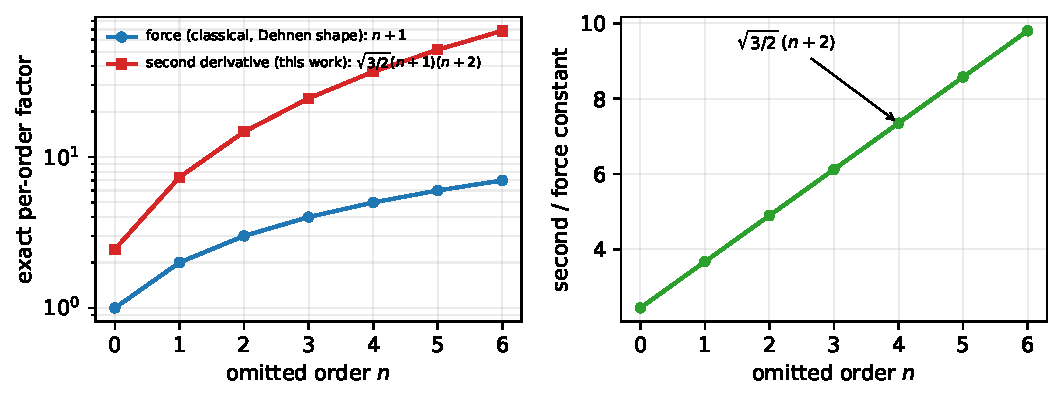
\includegraphics[width=\columnwidth]{figures/fig_dehnen_vs_second.pdf}
\caption{Schematic comparison of the exact per-order factors, not a new measurement. Both
remainders carry $(R/r)^n$; the second derivative adds one power of $1/r$ and a factor
$\sqrt{3/2}(n+2)$ relative to the classical force remainder. Constants are those derived and
verified in Appendix~\ref{app:secondorder}.}
\label{fig:dehnen}
\end{figure}

\section{Experiments}

\noindent Every experiment below uses the protocol of Section~\ref{sec:protocol}: real CAMELS
$L25n256$ particles, the brute-force exact sum as ground truth, and $\theta=0.5$ unless a setting
is stated. Every number is produced by a script in the accompanying repository
(Appendix~\ref{app:repro}).

\noindent\textbf{Two disclosed corrections sit behind every number below.} Defect~D6 (the
second-derivative reference was not the second derivative, and no quadrupole contribution to it
existed) and defect~D8 (the octree's recorded cell centres were offset by a full cell side) both
invalidated earlier measurements and are both corrected here. The full disclosure --- including how
each defect survived the tests that existed at the time --- is Appendix~\ref{app:provenance}, and is
not repeated below. Two consequences are load-bearing for reading the tables: every operator number
is post-D8, and the pre-D8 values were $10$--$41\times$ larger; and the failure mode one would otherwise expect at large opening angles \emph{is} D8 itself rather than a property of the approximation, which is why this paper has no failure-mode section.

\subsection{Agreement with exact N-body forces}\label{sec:exact}
On $N=2{,}000$ particles the \emph{complete} operator --- exact near-leaf sums plus the truncated
monopole far field --- matches the brute-force exact Newtonian acceleration with global relative
error $0.001996$ and direction cosine $0.999998$ (Table~\ref{tab:exact}). We are explicit about
what this does and does not establish. It is a \emph{small-scale} check: at $N=2{,}000$ the octree
is shallow and few far cells are ever admitted, so it shows the near/far split reconstructs the
force correctly at that depth. It does \emph{not} show that the operator attains $0.2\%$ accuracy at
$N=2.3$M, and we do not claim that.

\begin{table}[h]
\centering
\caption{Agreement with a brute-force exact N-body force ($N=2{,}000$, $\theta=0.5$, softening
$\epsilon=10^{-4}$; \protect\path{scripts/exact_nbody.py}). Measured on synthetic lognormal clouds, the
same distribution as the order study of Section~\ref{sec:order}. \textbf{Every operator number in
this paper is post-defect-D8} (Appendix~\ref{app:provenance}). The pre-fix value, and what the correction was worth, are in Appendix~\ref{app:provenance}. The stored
artifact keys are named \texttt{far\_field\_*}, but the measured quantity is the \emph{complete}
operator ($a^{\mathrm{far}}+a^{\mathrm{leaf}}$), never the far field alone. The global error is the
ratio of field norms, not a per-particle mean.}\label{tab:exact}
\begin{tabular}{lr}
\toprule
Quantity & Value \\
\midrule
Global relative force error & $0.001996$ \\
Direction cosine & $0.999998$ \\
\bottomrule
\end{tabular}
\end{table}

\noindent\textbf{At $N=2{,}000$ the tree is not yet paying for itself} ($0.0758$\,s against
$0.0795$\,s for the direct sum on one CPU core). Barnes--Hut buys asymptotic scaling, not small-$N$
speed. This is the low end of a crossover we now measure rather than bracket: on the same CPU
configuration it arrives at $N\approx6{,}000$--$8{,}000$, and Section~\ref{sec:scaling} gives the
ladder, the sampled-reference comparison and the hardware caveat. Single-run wall-clock on a shared
machine carries tens of percent of noise, so the two numbers above are read as ``no advantage yet''
rather than as a measured ratio --- at this $N$ they differ by less than the noise.

\noindent\textbf{At shallow depth the near-leaf sums carry most of the residual.} At the same $N$
and $\theta$, the monopole \emph{far field alone} has mean per-particle relative error $0.041258$
and mean cosine $0.999254$. \textbf{These two pairs of numbers come from different scripts and use
different error definitions} --- a global norm ratio for the complete operator versus a
per-particle mean for the far field --- so they are indicative rather than a like-for-like
ablation. We quote them for one narrow point only: the exact near-leaf contribution, not the
multipole order, is what dominates the remaining error at shallow tree depth.

\subsection{Validation at 2.3M particles by sampled queries}\label{sec:scale}

The small-scale check above verifies the near/far split at shallow depth. To verify the operator at
the scale it is meant for, we use the fact that the brute-force reference has to be evaluated only
at the nodes for which an error is reported: restricting the octree descent to a sampled query set
$Q$ makes the reference cost $O(QN)$ instead of $O(N^{2})$, which is affordable at $N=2.3$M. We
report two quantities at those nodes, both against their own brute-force sum: the acceleration, and
the \emph{tidal tensor}
\begin{equation}
T_{ij}=\frac{\partial a_i}{\partial x_j}=-\frac{\partial^{2}\phi}{\partial x_i\partial x_j}
=\sum_j m_j\Big[\frac{3d_id_j}{r^{5}}-\frac{\delta_{ij}}{r^{3}}\Big],\qquad d=x_j-x_i ,
\label{eq:tidaldef}
\end{equation}
with the sign fixed by $a=-\nabla\phi$: \textbf{the tidal tensor is minus the Hessian of the
potential}, and it is the Jacobian of the force that a vector--Jacobian product actually
differentiates. We use ``tidal tensor'' for this object, and only this object, throughout; where
the literature's opposite sign convention appears we say so. Both are measured on the \emph{complete} operator, and because the
near-leaf sums are exact they cancel identically in the difference, so every entry below is a pure
far-field truncation remainder.

The bound of Appendix~\ref{app:secondorder} is verified on the same configuration. At $\theta=0.5$
with $2{,}048$ query nodes the tree admits \textbf{$1{,}643{,}251$} far interactions and the bound
holds on every sampled node there (\protect\path{bound_f64_com_2M3.json}), at a \textbf{median looseness
of $426\times$} (tightest $30\times$, worst $2534\times$). The same test run on the \emph{whole}
$16.7$M snapshot --- deliberately the same $N$ as the operator table below, so that bound and operator
are verified at one scale rather than two --- admits $1{,}060{,}190$ far interactions over
$3{,}927{,}827$ cells, samples $1{,}024$ nodes, and again finds \textbf{zero violations}, at a median
looseness of \textbf{$436\times$}. The looseness chain is $186\times\to306\times\to426\times\to436\times$
from $4$k to $16.7$M: it grows with scale and is \emph{saturating}, which is the signature of a bound
whose exponent is right --- a bound with the wrong power of $r$ would drift without limit instead.
\textbf{That test is evaluated in float64, and it has to be}: the
same $2.3$M configuration in float32 reports \emph{two} spurious violations and a looseness of
$32.6\times$ where float64 reports none and $425.6\times$, with every bound-side quantity agreeing to
six significant figures and the tail share bit-identical (Appendix~\ref{app:secondorder}). A
round-off artefact is indistinguishable from a violation unless the precision is stated, so it is
stated here rather than only in the appendix.

The tidal reference is an independent implementation that is pinned to \texttt{torch.autograd}'s
Jacobian of the exact force to $10^{-10}$ in double precision (\protect\path{tests/test_tidal_tensor.py});
this matters, because an earlier version of this paper used a second-derivative expression that was
\emph{not} the Jacobian and understated the tidal error by a factor of $\approx2.7$. That defect is
disclosed as (D6) in Appendix~\ref{app:provenance} and every number in Table~\ref{tab:sampled} is
from after the fix.

\begin{figure}[t]
\centering
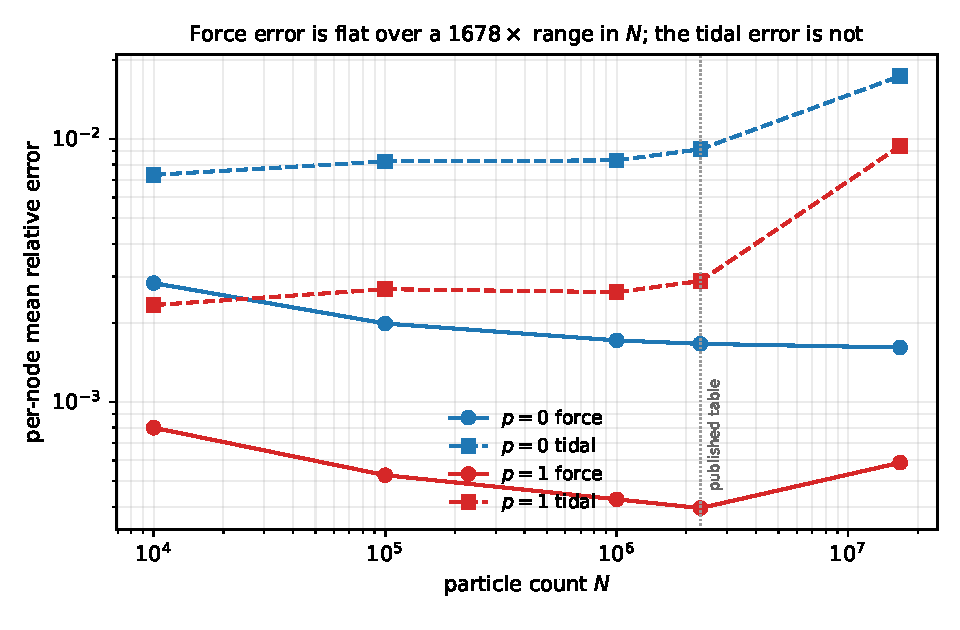
\includegraphics[width=\columnwidth]{figures/fig_error_vs_N.pdf}
\caption{Per-node mean relative error against particle count, both multipole orders, force and tidal,
for the published rows of Table~\ref{tab:sampled} (\protect\path{scripts/make_paper_figures.py}). The force
error is almost flat across a $1678\times$ range in $N$: a factor $1.7$ with the monopole and $2.0$
with the quadrupole. \textbf{The tidal error is not flat at the top of the range} --- $2.4\times$ and
$4.0\times$ over the full span, against $1.3\times$ over the first $230\times$ --- because the admitted
cell population changes with $N$. Light bars mark the second query-set size where one exists, which
moves nothing.}\label{fig:errorN}
\end{figure}

\begin{table}[t]
\centering\small
\caption{Complete operator against brute-force exact N-body values at sampled query nodes, real
CAMELS $L25n256$ snapshot, $\theta=0.5$, $\epsilon=10^{-4}$, $\texttt{max\_leaf}=16$; the last row of
each block uses the full $16.7$M snapshot, at the single query count $Q{=}1024$ used by the
eleven-draw error-bar campaign of Section~\ref{sec:scale}. Entries are per-node mean relative errors;
$T/F$ is the tidal-to-force ratio. $p{=}1$ adds the quadrupole, whose
contribution to the tidal tensor is the derivative of the same quadrupole term.
\textbf{The force} error varies by only a factor $1.7$ ($p{=}0$) and $2.0$ ($p{=}1$) over a
$1678\times$ range in $N$. The tidal error is flatter still out to $2.3$M and then rises, which is why
$T/F$ jumps in the last row ($5.28\to10.76$ and $7.02\to15.97$): that rise is the second derivative's
error growing relative to the force's with $N$, the quantitative content of Dehnen's qualitative
remark, and \emph{not} a loss of convergence (Section~\ref{sec:scale}). Sampling uncertainty is
$1.2$--$1.7\%$ on the $2.3$M rows and $2.0$--$7.3\%$ on the
$16.7$M rows, largest for the force mean, whose per-node error is heavy-tailed (Section~\ref{sec:scale}, eleven draws); both
order-dependence statements below are insensitive to it.}\label{tab:sampled}
\begin{tabular}{lrrrr}
\toprule
\multicolumn{5}{l}{\textbf{$p{=}0$ (monopole far field)}} \\
$N$ & $Q$ & force & tidal & $T/F$ \\
\midrule
$10{,}000$     & $512$  & 0.002834 & 0.007310 & 2.58 \\
$100{,}000$    & $2{,}048$ & 0.001990 & 0.008233 & 4.14 \\
$1{,}000{,}000$ & $2{,}048$ & 0.001716 & 0.008306 & 4.84 \\
$2{,}300{,}000$ & $1{,}024$ & 0.001666 & 0.009149 & 5.49 \\
$2{,}300{,}000$ & $2{,}048$ & 0.001704 & 0.009005 & 5.28 \\
$16{,}777{,}216$ & $1{,}024$ & 0.001613 & 0.017358 & 10.76 \\
\midrule
\multicolumn{5}{l}{\textbf{$p{=}1$ (monopole $+$ quadrupole)}} \\
$N$ & $Q$ & force & tidal & $T/F$ \\
\midrule
$10{,}000$     & $512$  & 0.000799 & 0.002337 & 2.93 \\
$100{,}000$    & $2{,}048$ & 0.000528 & 0.002687 & 5.09 \\
$1{,}000{,}000$ & $2{,}048$ & 0.000427 & 0.002618 & 6.13 \\
$2{,}300{,}000$ & $1{,}024$ & 0.000395 & 0.002886 & 7.30 \\
$2{,}300{,}000$ & $2{,}048$ & 0.000424 & 0.002976 & 7.02 \\
$16{,}777{,}216$ & $1{,}024$ & 0.000588 & 0.009400 & 15.97 \\
\bottomrule
\end{tabular}
\end{table}

Three things follow. \textbf{(a) Accuracy depends only weakly on $N$} at fixed $\theta$: across the full $1678\times$ range the force error moves by a factor $1.7$ with the monopole and $2.0$ with the quadrupole. The tidal error is flatter still out to $2.3$M ($1.3\times$ either way) and then rises at the largest $N$, to $2.4\times$ and $4.0\times$ over the full range --- which is the growth of the tidal-to-force ratio in (b) below, not a loss of convergence; out to $2.3$M the tendency is for the error to \emph{improve} with $N$ rather than degrade --- so the operator's error is set by the opening angle,
as the bound says, with a residual $N$-dependence coming from the composition of the admitted cell
population rather than from the particle count. \textbf{(b) The second derivative is worse than the
force by a factor that grows with $N$}: $2.6$--$5.5$ with the monopole and $2.9$--$7.3$ with the
quadrupole over $10^{4}$--$2.3$M, rising to $10.8$ and $16.0$ on the $16.7$M snapshot. That is the
quantitative content of Dehnen's qualitative remark~\citep{dehnen2014fmm}, and the growth is the
sharper half of it: a gradient-based consumer's margin over a force-only one is not a constant that
can be read off a single run. \textbf{(c) The quadrupole improves both, by substantially more than
this paper previously reported}: $3.0$--$4.2\times$ on the force and $3.0$--$3.2\times$ on the tidal
at $\theta=0.5$. The order
dependence of Section~\ref{sec:order} pays off at full scale by a factor of three or more.

The direction cosines are $0.999999$--$1.000000$ for the force and $\ge0.9999999$ for the tidal
tensor across the whole range, with no trend in $N$. The per-node mean is
nevertheless the statistic to read, and the reason is worth stating
because the same trap catches the \emph{global} relative error: at $16.7$M the quadrupole
\emph{worsens} the global force ratio ($2.5\times10^{-3}$ against $8.6\times10^{-4}$) while
\emph{improving} the per-node mean by $2.7\times$ ($5.9\times10^{-4}$ against $1.6\times10^{-3}$) and
the $90$th percentile by $3.6\times$. A norm ratio over all nodes is dominated by a handful of outlier
nodes, so it can invert the ordering that the per-node statistics agree on. Per-node statistics on the
tidal tensor, and norm-weighted ones on either quantity, are outlier-dominated
(Section~\ref{sec:limits}) --- which is the same argument as
Section~\ref{sec:meanisnotbound}, one statistic over.

\noindent\textbf{How much of this is sampling?} The $2.3$M rows are a sample of $Q=2{,}048$ nodes, so
they carry a sampling uncertainty. Re-drawing the query set five times with the particle set fixed
(Appendix~\ref{app:repro}) gives $1.2$--$1.7\%$ relative, several times smaller than any difference we
draw between configurations. \textbf{The $16.7$M rows are more sampling-limited, and not uniformly
so.} Re-drawing only their query set at the published configuration ($Q=1{,}024$, eleven draws, of
which the published row is one) gives $7.3\%$ for the $p{=}0$ force, $6.4\%$ for the $p{=}1$ force,
$2.0\%$ for the $p{=}0$ tidal error and $2.3\%$ for $p{=}1$ tidal --- relative standard deviation,
with every published value sitting within $1\sigma$ of the eleven-draw mean. \textbf{The force rows
are the sampling-limited ones, and the reason is the heavy tail}: at $16.7$M the $p{=}1$ force has
median/mean $=0.55$ and max/mean $=142$, so its mean is set by rare nodes rather than by the typical
one. We therefore state the order and $N$ dependence as \emph{factors} rather than as absolute values,
and have checked that the $16.7$M rows, which carry the largest spread, are neither the maximum nor
the minimum of any factor we quote: the factor-$1.7$ and factor-$2.0$ statements are unchanged if both
rows move by their full spread. \emph{The sampling budget itself matters here: three draws at
$Q=2{,}048$ would have put $0.2\%$ on the $p{=}0$ force --- a $36\times$ under-estimate from too few
draws --- which is why the eleven draws above use $Q=1{,}024$ instead.}

\subsection{Physical fidelity of the second derivative}\label{sec:physics}

A Frobenius-norm error is not the quantity that makes a tidal tensor useful. What it is used for is
the local classification of the environment and the orientation of the principal axis, so we measure
per-eigenvalue error, principal-axis misalignment, and the fraction of nodes whose eigenvalue-sign
class changes (Table~\ref{tab:eigen}, Appendix~\ref{app:surface}). \textbf{That class is binary, not
the usual four-class scheme that descends from Zel'dovich's classification~\citep{zeldovich1970}}: the
tensor is traceless, so it has only one or two positive eigenvalues
(Appendix~\ref{app:surface}, check 5). \textbf{At the operating point the approximate tensor changes
the class for $0.10$--$1.4\%$ of nodes}, and the worst-conditioned $5\%$ have their principal axis
wrong by at most $2.6^{\circ}$ . The
exact mixture is $71\%$ sheet-like and $29\%$ filament-like, so a flip crosses the dominant
population boundary. Raising the order helps but does not fix it ($0.51\%\to0.27\%$ at $2.3$M);
\textbf{changing the acceptance test does not} --- post-D8 the centre-of-mass and distance-to-cell
tests agree to a few per cent, and at $\theta=0.70$ the class-flip rate is \emph{identical} for both
($1.39\%$).

\noindent\textbf{Does the error land where it matters?} A flip in an empty region costs nothing; one
on a filament spine is a statement about where galaxies form. Weighting the measurement by a $k$-NN
density proxy (Appendix~\ref{app:environment}), the flip rate runs from $6.5\%$ in the lowest-density
octile to $5.1\%$ in the highest, non-monotonically, with the class mixture flat at $76$--$82\%$
sheet-like throughout. \textbf{We find no evidence that the error concentrates where it matters} ---
it is close to uniform --- but this snapshot is at $z\approx6$, where the density contrast is mild.

\subsection{The gradient a field-level reconstruction uses}\label{sec:vjp}

Reconstructing initial conditions from a present-day field means differentiating through the gravity
solver, and the resulting gradient is a vector--Jacobian product whose kernel is the tidal tensor of
Section~\ref{sec:physics}. A VJP contracts the per-node Jacobians with an adjoint vector and
\emph{sums}, so it can amplify the per-node tidal error coherently or cancel it, and the per-node
number says nothing about which. We therefore differentiate the density-weighted tidal energy
$L(w)=\sum_i w_i\|T_i\|_F^2$, with $w_i$ a $k$-NN density proxy, through the exact field and through
the operator, and report the \emph{amplification factor} $\|\hat{g}-g\|/\|g\|$ over the per-node
tidal error \textbf{at the same multipole order} and weighted by $\|T\|^2$: the latter because that
is what $L$ is made of (norm-weighted statistics are outlier-dominated, Section~\ref{sec:limits}),
the former because the $p{=}0$ and $p{=}1$ tensor errors differ by more than the effect being
measured. Synthetic lognormal clouds, $N=10^{5}$, $Q=256$, $p{=}0$, $15$ seeds per cell:

\begin{table}[t]
\centering\small
\caption{Gradient error through the complete operator, density-weighted $L$, $p{=}0$, $N=10^{5}$,
$Q=256$, $15$ seeds per cell, synthetic lognormal clouds, both acceptance criteria ---
centre-of-mass (\texttt{com}) and geometric-centre (\texttt{geo}), defined in
Appendix~\ref{app:surface} --- both post-defect-D8. \textbf{The VJP contracts rather than amplifies}: the amplification factor --- the
gradient error over the $\|T\|^2$-weighted per-node tidal error at the same multipole order --- is
below one in every $p{=}0$ configuration we measured, maximum $0.76$, so the gradient a reconstruction actually descends on is
\emph{more} accurate than the tensor it came from. There are no failures at any $\theta$ tested.
All entries measured, none fitted.}\label{tab:vjp}
\begin{tabular}{llrrrrr}
\toprule
criterion & $\theta$ & grad.\ rel.\ err (med / max) & $\cos$ (min) & amp.\ (med / max) & amp.${>}1$ & failures \\
\midrule
com  & 0.50 & $1.4\times10^{-4}$ / $1.4\times10^{-3}$ & $0.999999$ & $0.25$ / $0.76$ & 0 & 0 \\
com  & 0.70 & $3.1\times10^{-4}$ / $5.2\times10^{-3}$ & $0.999992$ & $0.20$ / $0.67$ & 0 & 0 \\
\midrule
geo  & 0.50 & $1.6\times10^{-4}$ / $1.2\times10^{-3}$ & $1.000000$ & $0.22$ / $0.65$ & 0 & 0 \\
geo  & 0.70 & $3.5\times10^{-4}$ / $5.4\times10^{-3}$ & $0.999993$ & $0.21$ / $0.67$ & 0 & 0 \\
\bottomrule
\end{tabular}
\end{table}

\noindent\textbf{Precision of the median column.} The medians above are quoted to two significant
figures deliberately. The underlying statistic is a float32 difference of two gradients whose norms
are $\sim10^{4}$ times the difference itself, and the $15$ seeds cluster tightly enough that
re-running the \emph{identical} configuration --- same cloud, byte-identical input file, same seeds,
same source --- on a second platform with a different PyTorch build moves individual seeds by up to
$50\%$ (worst on the smallest draws) and the $15$-seed median by $30\%$: $1.1\times10^{-4}$ there
against $1.4\times10^{-4}$ here for the \texttt{com}, $\theta=0.50$ row. The maxima move by a few per
cent, and every conclusion drawn above --- every amplification factor below one, no failures,
$\cos\ge0.99999$ --- is unchanged. A third significant figure on a median here would be noise, so we
do not quote one. An independent $15$-seed run on a
different platform reproduces every maximum to a few per cent and moves the medians within the
spread quoted above, which is why the two are quoted at the precision they are.

\noindent\textbf{The per-node tidal error is a conservative proxy for the gradient error.} The
amplification factor stays below one in every $p{=}0$ configuration we measured, with a maximum of $0.76$.
The per-node errors partially cancel in the adjoint sum, so quoting the per-node tidal error as the
error of a reconstruction errs on the safe side --- a direction that favours the operator, and that
we did not assume going in. This is the quantitative form of the differentiability claim in
Appendix~\ref{app:diff}, and it is the property a field-level inference actually consumes.

\noindent\textbf{And it holds on real data, not only on clouds.} Table~\ref{tab:vjp} is entirely
synthetic, so we repeated the measurement on the CAMELS \texttt{L25n256} snapshot --- the same data
the operator validation uses --- over $N\in\{2\times10^{4},10^{5}\}$, $\theta\in\{0.50,0.70\}$, both
acceptance criteria, both multipole orders and three seeds per cell, giving $48$ density-weighted
configurations (\protect\path{scripts/eval_vjp_error.py},
\protect\path{outputs/vjp_camels_real_data.json}). \textbf{The amplification is below one in all $48$},
from $0.226$ to $0.766$ with a median of $0.510$; the gradient's relative error stays at or below
$1.7\times10^{-4}$ and its direction cosine at or above $0.99999982$. The contraction is therefore not
an artefact of controlled clouds: on real clustering, with its heavy tails, the gradient a
reconstruction descends on is still \emph{more} accurate than the tensor it came from, by about a
factor of two.

\noindent\textbf{The gradient is not where the error concentrates.} Its median relative error at
$\theta=0.70$ is $3.3\times10^{-4}$, roughly a fifth of the $\|T\|^2$-weighted per-node tidal error
it is built from ($1.5\times10^{-3}$), and its direction cosine stays above $0.99999$ at every
setting. A user who budgets from the tensor error will over-provision, not under-provision.

\noindent\textbf{Does the contraction survive being \emph{used}?} An amplification factor is an
error-propagation statistic, not a promise that an optimiser will converge, so we test the downstream
question directly rather than inferring it. We perturb a known cloud, define a density-weighted
tidal-energy objective, and minimise it by gradient descent \emph{through the operator} for $30$
iterations, at two particle counts and three opening angles. The gradient direction is exact to
measurement precision --- $\cos(\hat g,g_{\mathrm{exact}})=1.000000$ in all six arms --- and the loss
falls by $68\times$ ($\text{final}/\text{initial}=0.0146$--$0.0147$). The informative part is what
does \emph{not} track it: the amplification factor spans $3.1\times$ across these arms ($0.269$ to
$0.835$) while the convergence ratio is flat to $0.7\%$, and the $\|T\|^{2}$-weighted per-node tidal
error spans two decades ($3.5\times10^{-6}$ to $4.3\times10^{-4}$). \textbf{So the per-node
amplification factor does not predict downstream convergence}, and we do not claim that it does. What
it bounds is the \emph{error} the adjoint delivers, which is what a reconstruction's accuracy rests
on; how fast a particular optimiser descends is a separate question that this measurement shows to be
insensitive to it. Both statements are usable and they are different statements. \textbf{This does
not weaken the contraction result; it delimits it.}

\noindent\textbf{Why JZ-FMM report that gradients need higher accuracy, and why that is compatible
with the contraction above.} Their finding is that the position gradient converges more slowly than
the force --- $\lesssim10^{-3}$ against $\lesssim10^{-2}$ at $p=5$ --- and we reproduce the pattern
qualitatively. The two results are anchored differently and must not be read as a disagreement: their
figures are tail-like statistics over the particle set (a per-particle error distribution, and a
$90$th percentile at scale), while the amplification here is a ratio of \emph{means} over
$\|T\|^{2}$-weighted nodes, and Section~\ref{sec:meanisnotbound} measures the same quantity to differ
by $10$--$35\times$ between the mean and the worst case. \emph{Theirs is a statement about the tail
and ours about the mean, and both hold.} We state the distinction explicitly because the opposite
reading --- that a contracting adjoint licenses the same $\theta$ as the force --- is precisely the
inference this paper's worst-case section exists to block.

\noindent\textbf{The acceptance criterion is a performance question, not a correctness one.} With
the octree geometry corrected (defect D8, Appendix~\ref{app:provenance}) both acceptance tests are
well behaved at every $\theta$ we tested, $\theta=0.70$ included; the distance-to-the-centre-of-mass
test --- the published one --- is marginally the more accurate. Before the geometry fix this
subsection read very differently: the geometric-centre test produced gradient errors of
$4.6\times10^{-2}$ with a direction cosine of $0.000000$ on $5$ of $15$ seeds, and it was that
failure which led us to the defect.

\subsection{Multipole-order validation}\label{sec:order}

\emph{A direct force-error test of the order dependence.} The layer-count factor and the absolute
constant are out of reach, but the \emph{order} dependence is not: raising $p$ by one multiplies
the truncation error by $R/r$, and because a Barnes--Hut cell is admitted only when
$R/r<\theta$, the ratio of consecutive-order errors must be proportional to $1/\theta$. We test
this on the \emph{complete} physical operator --- exact near-leaf sums plus the truncated far
field, against a brute-force exact $O(N^2)$ N-body force on the same particles and the same
tree.

\begin{table}[t]
\centering\small
\caption{Direct force-error validation of the multipole-order prediction, on synthetic lognormal
particle clouds (particles importance-sampled from a $32^{3}$ Gaussian field, box $100$). Entries are the
measured ratio of complete-operator errors, $p{=}0$ (monopole only) over $p{=}1$
(monopole $+$ quadrupole), multiplied by $\theta$. Proposition~\ref{prop:bound} predicts this product to
be \emph{constant} in $\theta$: over all $21$ settings
($N\in\{2{,}000,\,8{,}000,\,32{,}000\}$, $\theta\in[0.15,0.60]$) it is
$2.374879\pm0.117030$, a relative scatter of $4.93\%$. \textbf{The structure survives --- the
product is constant to within its scatter and the ratio exceeds one everywhere --- but the constant
itself doubled when we corrected the octree geometry} (defect D8, Appendix~\ref{app:provenance}:
the pre-fix value on the same grid was $1.171830$). \textbf{It is a property of this particle
distribution and not a universal number}: on the real CAMELS snapshot the same product varies by
$1.6$--$1.9\times$ across the same $\theta$ range, and the \emph{tidal} product's scatter there grows
with $N$ until it is no longer measurable (Table~\ref{tab:camelsorder}). All entries are measured,
none fitted.}\label{tab:ordersweep}
\begin{tabular}{lrrr}
\toprule
$\theta$ & $N=2{,}000$ & $N=8{,}000$ & $N=32{,}000$ \\
\midrule
0.15 & 2.943519 & 2.161378 & 2.588901 \\
0.20 & 2.843971 & 2.142369 & 2.445087 \\
0.25 & 2.783794 & 2.118240 & 2.303131 \\
0.30 & 2.565689 & 2.174436 & 2.315238 \\
0.40 & 2.412688 & 2.238519 & 2.355897 \\
0.50 & 2.247272 & 2.219304 & 2.280362 \\
0.60 & 2.297805 & 2.225078 & 2.209595 \\
\bottomrule
\end{tabular}
\end{table}

\noindent At the operating point $\theta=0.5$ the quadrupole cuts the relative force error
from $0.038582$/$0.040265$/$0.041258$ to $0.016101$/$0.016555$/$0.018094$ for
$N=32{,}000$/$8{,}000$/$2{,}000$ --- a factor of $2.28$--$2.43$ --- and raises the direction
cosine from $\approx0.99927$ to $\approx0.99984$. That is the payoff of the order dependence the
bound predicts, and it is cheap but \emph{not} free: measured on the complete operator at $2.3$M
(Table~\ref{tab:sampled}), retaining the quadrupole costs $1.36\times$ ($0.191$\,s to $0.260$\,s at
$Q=2{,}048$) for a $1.4$--$1.5\times$ accuracy gain. The quadrupole moments themselves are already
computed for every cell, so the extra cost is the added far-field arithmetic, not a new moment.
The default operator throughout this paper nevertheless remains $p=0$
(monopole only), so that the configuration validated here is the same one used in
Section~\ref{sec:exact}; we do not switch the operator between sections.

\noindent\textbf{The same test for the second derivative.} We repeat the sweep with the
\emph{tidal tensor} as the target, on the same tree, the same interaction list and the same query
nodes --- only the derivative count changes. This required implementing the quadrupole contribution
to the tidal tensor (one more derivative of the same term, verified against \texttt{torch.autograd}
rather than against a re-derived formula, because the re-derived formula had been wrong; defect (D6)).
The product is again approximately constant, at a different value:

\noindent The per-$\theta$ means (over $N\in\{2{,}000,8{,}000,32{,}000\}$) are tabulated in
Appendix~\ref{app:percell}. The tidal product averages
$1.774$ over $\theta\le0.5$ with a relative scatter of $2.9\%$, against $2.391$ and $4.3\%$ for the
force on the same grid --- so the second derivative's order shift is \emph{more} stable than the
force's here, not less. \textbf{On clouds of this character the order shift survives
differentiation}: the omitted term is
again one order above the retained one, so a second-derivative remainder of the classical shape with
an explicit order shift is the right target --- though on real data at scale only the \emph{sign} of
that shift survives, as the next paragraph measures. Two different numbers live here and must not be
conflated. The \emph{bound's} constant ratio is what the lemmas fix, and with the sharp
second-derivative constant $\sqrt{3/2}(n{+}1)(n{+}2)$ the ratio of the $p{=}0$ and $p{=}1$ constants
is $(3\cdot4)/(4\cdot5)=0.6$ --- so the $(n{+}1)(n{+}2)$ structure is the right one, and it predicts
a bound-constant ratio near $0.6$, not $1.8$. The measured product $1.774$ is an \emph{aggregate over
admitted cells}, not a bound constant; being about $3\times$ above the bound is exactly what a valid
bound requires, and it is the same $3.3\times$ looseness the force column shows. The measured
$\theta$-power of the leading \emph{absolute} error is $2.98$ for the force and $3.39$ for the tidal
tensor, and of the \emph{relative} error $3.23$ and $3.56$ (Appendix~\ref{app:provenance}, D6); the
two pairs differ because one is normalised by the field magnitude and the other is not, and neither
pair is the bound's own $\theta^{p+2}$. Either way the force and tidal powers agree to within $0.4$,
so we find \emph{no} anomalous scaling for the second derivative.

\noindent\textbf{Qualification: this constant characterises the clouds it was measured on, and on real
data the second derivative's version of it does not survive at scale.} All of
Table~\ref{tab:ordersweep} and both columns above come from synthetic lognormal clouds. Repeating the
sweep on the real CAMELS snapshot --- same $\theta\in[0.15,0.60]$ range, $Q=2{,}048$ query nodes,
post-D8 --- gives Table~\ref{tab:camelsorder}: the $\theta$-weighted product is not constant there for
either derivative, and the tidal one degrades with $N$ until its scatter is the same size as the
effect it is supposed to describe.

\noindent Three readings, and the third is a limit on what this section can claim.
\textbf{(i) The constant is a property of the mass distribution}: the force product varies by
$1.6$--$1.9\times$ across $\theta$ at each of the three scales, with relative scatters of
$15.7$, $24.4$ and $23.5\%$ --- so no single number transfers from the controlled clouds to this
snapshot, and the scatters do not shrink with $N$. \textbf{(ii) The ordering between the two
derivatives inverts with scale.} At $N=10^{5}$ the tidal product is the \emph{more} stable of the two
($3.9\%$ against $15.7\%$), the opposite of the controlled-cloud ordering; by $N=10^{6}$ it is the
less stable one ($35.7\%$), and by $2.3$M its scatter is $53.9\%$ and its product moves over an
$8.1\times$ range across $\theta$ ($0.208$ at $\theta=0.15$ to $1.682$ at $\theta=0.50$).
\textbf{(iii) At the scale this paper is about, the tidal order shift is a direction and not a
constant.} What survives at every scale and in every configuration we ran is the \emph{sign}: the
$p{=}0$ over $p{=}1$ error ratio exceeds one in all $21$ real-data configurations for both the force
(ratio $4.0$--$24.5$) and the tidal tensor (ratio $1.4$--$12.1$), so retaining the quadrupole always
helps. The constant, however, transfers only between datasets of the same character, and on this
snapshot at $2.3$M it is not resolved at all. We report the sign as the robust result and the
constant as a cloud-specific one rather than quoting a single number for both.

\noindent\textbf{What this does and does not say about a universal constant.} A bound is built
\emph{per interaction}, whereas the numbers above are aggregates over cells and nodes, so we
recomputed the same interaction list at three aggregation levels (Appendix~\ref{app:percell}): all
three agree and are constant on the controlled cloud, and all three drift on the real snapshot. The
drift is therefore not merely an aggregation artefact. \textbf{We then asked the single-cell question
directly --- does the one-order inequality $\varepsilon_1\le C\rho\varepsilon_0$ survive being
calibrated somewhere other than where it is checked? --- and it has a sharper answer than either
outcome we anticipated.} On controlled cells that inequality does hold, with $K$ bounded above
(maximum $59.6$ for the tidal tensor), but $C=1/\min K$ fitted on the same cells it is then evaluated
on is a fit rather than a bound, so we calibrated on nine cell geometries and tested the tenth, and
separately calibrated on some random seeds and tested a fresh one. \textbf{The constant is carried by
a single geometry: the spherical shell.} Nine held-out geometries of ten are covered with room to
spare, while the shell violates the calibrated bound at $13$ of $90$ held-out samples and forces $C$
up by $2.3\times$ (tidal) and $4.4\times$ (force); a fresh \emph{seed} of the stochastic families, by
contrast, transfers with no violations at all. The failure is therefore \emph{between geometries, not
between draws}, and the binding case is the configuration where the octupole term is weakest. So a
universal constant exists only in the weak sense that $\sup K$ is finite: a constant calibrated on
arbitrary clouds does not transfer to the near-degenerate ones. We report the scaling law per dataset
and the constant per family of cell geometries, which is the strongest claim the measurements
support (Appendix~\ref{app:percell}).

\subsection{The mean is not a bound}\label{sec:meanisnotbound}

Every second-derivative number quoted in this paper --- and, as far as we can read it, in the
literature it engages --- is an average, a percentile, or a distribution. A \emph{bound} is a
different kind of object: it is per interaction, and a sampler consuming the operator needs the
worst case, not the typical one. The gap is large and it is measurable on the same runs that produce
the averages, so we report it explicitly rather than leaving it implicit in a table caption.

\begin{figure}[t]
\centering
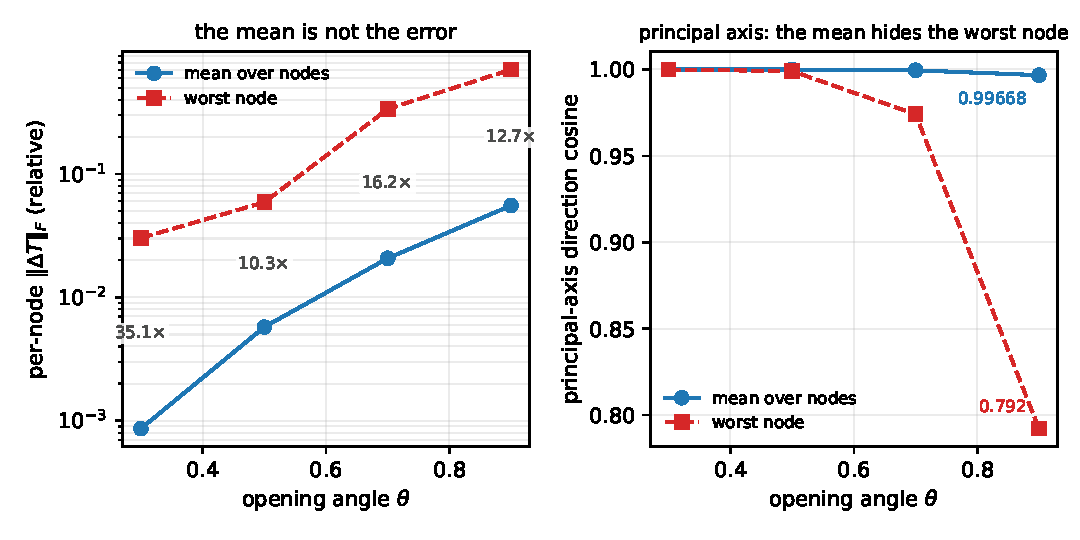
\includegraphics[width=\columnwidth]{figures/fig_mean_vs_worst.pdf}
\caption{The measurement behind Section~\ref{sec:meanisnotbound}, drawn
(\protect\path{scripts/make_paper_figures.py}). \emph{Left:} the per-node second-derivative error, mean
against the worst node, at each opening angle; the ratio is $10.3$--$35.1\times$ and is largest at the
tightest opening, so it is not a large-$\theta$ artefact a conservative user would avoid.
\emph{Right:} the principal-axis direction cosine, which at $\theta=0.90$ is $0.99668$ on average ---
visually perfect --- while the worst node sits at $0.792$. \textbf{Every quantity one would tabulate
is the mean; every quantity a step-size controller consumes is the worst node.}}\label{fig:meanworst}
\end{figure}

\begin{table}[t]
\centering\small
\caption{Mean against worst case for the same second-derivative measurement.
$N=20{,}000$, $Q=1{,}024$ query nodes, monopole order, synthetic lognormal cloud, reference the
brute-force sum. ``mean'' and ``worst'' are the mean and the maximum over query nodes of the
per-node relative error, the direction cosine of the principal axis, and the relative shift of the
largest eigenvalue. \textbf{Every quantity a practitioner would quote is the mean column; every
quantity a sampler's stability depends on is the worst column.} All entries measured, none fitted.}
\label{tab:meannotbound}
\begin{tabular}{rrrrrrr}
\toprule
& \multicolumn{2}{c}{per-node error} & \multicolumn{2}{c}{direction cosine} & \multicolumn{2}{c}{$\Delta\lambda_{\max}/\lambda_{\max}$} \\
\cmidrule(lr){2-3}\cmidrule(lr){4-5}\cmidrule(lr){6-7}
$\theta$ & mean & worst & mean & min & mean & max \\
\midrule
$0.30$ & $8.63\times10^{-4}$ & $3.03\times10^{-2}$ & $0.99999881$ & $0.99995446$ & $6.09\times10^{-4}$ & $9.83\times10^{-3}$ \\
$0.50$ & $5.75\times10^{-3}$ & $5.90\times10^{-2}$ & $0.99995917$ & $0.99902844$ & $3.51\times10^{-3}$ & $4.24\times10^{-2}$ \\
$0.70$ & $2.08\times10^{-2}$ & $3.36\times10^{-1}$ & $0.99952793$ & $0.97406769$ & $1.20\times10^{-2}$ & $1.73\times10^{-1}$ \\
$0.90$ & $5.56\times10^{-2}$ & $7.04\times10^{-1}$ & $0.99668145$ & $0.79209930$ & $2.96\times10^{-2}$ & $3.58\times10^{-1}$ \\
\midrule
worst/mean & \multicolumn{2}{c}{$10.3$--$35.1\times$} & \multicolumn{2}{c}{$0.9967 \to 0.792$} & \multicolumn{2}{c}{$12.1\times$} \\
\bottomrule
\end{tabular}
\end{table}

Three consequences, in increasing order of how much they matter.

\emph{The error is tail-dominated.} The worst node is $10.3$--$35.1\times$ worse than the mean, and
the ratio is not monotone in $\theta$ (it is largest at the tightest opening, $35.1\times$ at
$\theta=0.30$), so it is not a large-$\theta$ artefact that a conservative user would avoid anyway.
A percentile would hide this: at $\theta=0.90$ the mean relative error is $5.6\%$, which reads as
acceptable, while the worst node is at $70\%$.

\emph{Direction and eigenvalue are worse than the norm.} The Frobenius error is the quantity tables
usually quote; what a tidal classification or a step-size controller consumes is the principal axis
and the largest eigenvalue. At $\theta=0.90$ the mean direction cosine is $0.9967$ --- visually
perfect --- while the worst node is at $0.792$, i.e. a node whose principal axis is badly wrong, and
the relative shift of $\lambda_{\max}$ runs from $2.96\times10^{-2}$ on average to
$3.58\times10^{-1}$ at worst, a $12.1\times$ understatement. \textbf{A step size is set by
$\lambda_{\max}$}, and a bound on the bias of an inexact sampler has to hold uniformly in the
state, so the mean shift is not the quantity that controls anything.

\emph{The mean is a mean even of the things one would hope were structural.} The exact tidal tensor
is traceless, and it is tempting to assume the \emph{error} inherits that. It does not: the trace of
the error is $2.5\times10^{-5}$ of $\max|T|$ at every $\theta$ --- flat, as it must be if it is
dominated by the omitted trace-free multipole orders --- which is $1.2\%$ to $84.6\%$ of the error's
own Frobenius norm depending on $\theta$. So the error's tensor structure changes character with the
opening angle even though its trace stays negligible in absolute terms.

\noindent\textbf{What this changes.} It is the reason this paper's deliverable is a \emph{proof} and
not a better statistic. Appendix~\ref{app:secondorder} bounds the second-derivative remainder per
interaction, with the order, the size-to-distance ratio and the cell's mass distribution and aspect
ratio entering explicitly, and it does so with constants that are exact rather than fitted. The
bound is loose ($11$--$48\times$ on controlled cells) but it is an upper bound, and loose is the
only direction that is safe: a bound that understates certifies the case it should have caught. The
next subsection is the record of our attempt to get the tight version cheaply, and of its failure.

\subsection{An error estimator is not a bound}\label{sec:selfcertify}

Everything above compares the operator against a brute-force sum. That is the strongest possible
reference and it is also the reason the scale claim is fragile: a reference costs $O(QN)$, so at
$2.3$M one can afford a \emph{sample} of nodes and not the field. Appendix~\ref{app:secondorder}
supplies the other half of the answer --- a provable per-interaction bound --- but a bound is loose
($11$--$48\times$ on controlled cells), so it certifies without predicting. There is a third option
that needs neither: \textbf{ask the operator for its own error.}

\emph{The hierarchical surplus.} Evaluate the \emph{same} interaction list at two truncation orders
and subtract:
\begin{equation}
s_L \;:=\; \hat a^{(L+2)}-\hat a^{(L)},
\qquad
\mathcal S_L \;:=\; \hat T^{(L+2)}-\hat T^{(L)} .
\end{equation}
$s_L$ is not a bound on the omitted term, it \emph{is} the omitted term (to leading order): the
order-$L$ error is the sum of the terms from $L{+}1$ upward, and $s_L$ is the first of them. The
geometric ratio of successive surpluses then closes the series, so the surplus both \emph{measures}
and \emph{corrects}:
\begin{equation}
\hat T^{(L)}-\hat T^{\mathrm{exact}}\;\approx\;\frac{\mathcal S_L}{\rho-1},
\qquad
\hat T^{\mathrm{Rich}}\;=\;\hat T^{(L)}+\frac{\mathcal S_L}{1-\rho},
\qquad
\rho\;=\;\frac{\langle \mathcal S_{L+2},\mathcal S_L\rangle}{\langle \mathcal S_L,\mathcal S_L\rangle}.
\label{eq:surplus}
\end{equation}
The ratio must be \emph{signed} and projected on $\mathcal S_L$: a ratio of magnitudes cannot tell a
converging series ($\rho>0$) from an alternating one ($\rho<0$), and the first version of this
measurement used the magnitude and therefore anti-corrected, reporting a gain \emph{below} one
(median $0.76\times$) that was an artefact of nothing but that sign.

\noindent\textbf{Measured.} One cell, 800 unit masses, queries on 12 directions at each radius,
orders $\{0,2,4,6\}$ on a fixed particle set, reference the brute-force tensor. Table~\ref{tab:surplus}
gives the outcome. \textbf{The surplus is the error}: $|\hat T^{(L)}-\hat T^{\rm exact}|/|\mathcal S_L|$
has median $1.008$ and range $[1.000,1.803]$, and its direction is anti-parallel to the error with
median alignment $0.998$ ($-1$ exactly would be $\hat T^{(L)}-\hat T^{\rm exact}=-\mathcal S_L$). So the
error bar costs one extra far-field pass on a list that already exists, and needs no reference, no
second tree and no change in asymptotic cost. The extrapolation of \eqref{eq:surplus} beats the plain
higher order by a median $1.24\times$ (minimum $0.68\times$, i.e.\ it can regress at the smallest
radius where $\rho$ is not small) --- a real but modest gain, and not the point. \textbf{The point is
the bar, not the extra order:} for a single isolated cell the surplus yields a per-node error
statement where the $O(QN)$ reference yields one only where it is evaluated. \textbf{That last
sentence is true of one cell and false of the operator, and we measured the difference rather than
asserting it} --- see ``Status'' below, which is the actual result of this subsection.

\begin{table}[t]
\centering\small
\caption{Self-certification by hierarchical surplus. One cell of 800 unit masses, aspect $1$, queries
on $12$ directions at each radius, orders $\{0,2,4,6\}$ on a fixed particle set, exact reference a
brute-force sum. ``size'' is $|\hat T^{(L)}-\hat T^{\rm exact}|/|\mathcal S_L|$ and ``align'' is
$-\cos(\hat T^{(L)}-\hat T^{\rm exact},\mathcal S_L)$; both should be $1$ if the surplus is the
error. ``gain'' is the error at order $L{+}2$ divided by the error of \eqref{eq:surplus}. The
extrapolation is a bonus; the certification is the size and align columns. All entries measured.}
\label{tab:surplus}
\begin{tabular}{rrrrr}
\toprule
$r/R$ & order $L$ & $|\hat T^{(L)}-\hat T^{\rm ex}|$ & size & align \\
\midrule
1.5  & 0 & $2.01\times10^{1}$  & 1.803 & 0.532 \\
2.0  & 0 & $3.59\times10^{0}$  & 1.306 & 0.773 \\
4.0  & 0 & $9.28\times10^{-2}$ & 1.028 & 0.974 \\
8.0  & 0 & $2.85\times10^{-3}$ & 1.003 & 0.997 \\
16.0 & 0 & $8.90\times10^{-5}$ & 1.000 & 0.9995 \\
1.5  & 2 & $1.72\times10^{1}$  & 1.074 & 0.989 \\
2.0  & 2 & $2.28\times10^{0}$  & 1.037 & 0.996 \\
4.0  & 2 & $1.96\times10^{-2}$ & 1.008 & 0.9996 \\
8.0  & 2 & $2.07\times10^{-4}$ & 1.001 & 1.0000 \\
16.0 & 2 & $2.70\times10^{-6}$ & 1.000 & 1.0000 \\
\bottomrule
\end{tabular}
\end{table}

\noindent\textbf{Status, stated precisely.} The measurement above is on a controlled single cell using
an expansion that is order-general by construction (the truncated potential is written directly as the
Legendre series and differentiated by \texttt{torch.autograd}), so orders $4$ and $6$ are available
without hand-deriving a hexadecapole term. \textbf{We then built the same test on the real tree} ---
one interaction list from the octree, held fixed, with the far field evaluated at orders
$\{0,2,4,6\}$ on that list (the shipped operator supports only $l\le2$ behind a boolean, so this
needed a new order-general far field, verified against the shipped one to $5.5\times10^{-5}$, the
float32 limit of the latter) --- \textbf{and it does not work either.} Per query node:

\begin{center}\small
\begin{tabular}{lrrrr}
\toprule
family & \multicolumn{2}{c}{per-node $|\text{err}|/|\mathcal S|$} & per-node $-\cos$ & bar calibration \\
 & median & worst node & median & median (worst node) \\
\midrule
\textbf{order} (list fixed) & $0.17$--$1.98$ & $1.8\times10^{5}$ & $-0.21$--$-0.01$ & $0.59$ ($8.5\times10^{5}$) \\
\textbf{angle} ($\theta$ ladder) & --- & $1.35$ & $\approx0.0$ & $3.43$ ($9.42$) \\
\bottomrule
\end{tabular}
\end{center}

\noindent That row is a \emph{sweep}, not a single tree: four sizes ($N=2\times10^{3}$ to $10^{5}$) and
$30$ seed-runs, $7{,}680$ sampled nodes, all committed
(\protect\path{outputs/selfcertify_order_across_N.json}). Three things it settles, one of which corrects
what a single draw suggests. \textbf{The failure is a property of the method, not of one tree}: it
reproduces at every size and in all $30$ runs. \textbf{But the bar is roughly honest at the
\emph{median}} --- the median-of-medians calibration is $0.59$, i.e. conservative by about
$1.7\times$, and only $9$ of $30$ runs have a median above one --- so an operator that reported its
median would look fine. \textbf{It is the tail that kills it}: the worst node reaches $8.5\times10^{5}$,
and the median alignment, $-0.21$ to $-0.01$, carries no sign information at all against the
single-cell $0.998$.

The surplus is an essentially exact estimator \emph{for one isolated interaction} and it does not
survive assembly. The reason is structural rather than a coding error: the assembled far-field error
at a node is a sum over many admitted cells with \emph{different} convergence ratios and largely
\emph{uncorrelated} error directions, so a single surplus vector cannot represent it, and one
unlucky borderline cell produces a large true error that the surplus does not flag. Both families
therefore \textbf{understate} the error at their worst nodes --- by five orders of magnitude in the
order family, and $\sim10$ in the angle family --- which is worse than no bar at all, because it
certifies the thing it should have caught. This is
``a mean is not a bound'' one level up: \textbf{an error estimator is not a bound either}, and the
fact that the obvious fix fails is the reason Appendix~\ref{app:secondorder} has to be a proof rather
than an estimator. The deliverable of this paper is the provable per-interaction bound plus the
external $O(QN)$ reference at $2.3$M, not a self-reported bar; the iterator and both failures are
kept in the repository (\protect\path{src/laniakea_hmmp/models/selfcertify.py},
\protect\path{scripts/selfcertify_surplus.py}, \protect\path{scripts/selfcertify_operator.py},
\protect\path{scripts/selfcertify_order_operator.py}) so that the negative result is reproducible rather
than asserted.

\subsection{Beyond accuracy: a neighbour cutoff, and the conservation laws}\label{sec:conservation}

Two questions the accuracy tables do not answer: is there a cheaper way to obtain the same field, and
is the approximate field a \emph{conservative} force field at all? \textbf{A $k$-NN cutoff at matched
cost} ($k=665$, the operator's terms per query node at $\theta=0.5$) loses $93\%$ of the force,
because gravity is long-ranged and truncation discards the monopole of everything beyond. At matched
cost the tree is $309\times$ better on the force and $18\times$ better on the tidal tensor --- less
lopsided than one might expect, since the tidal field is a \emph{difference} of forces to which a
distant, near-uniform mass distribution contributes little, but not the bare $1.6\times$ an earlier
measurement of ours gave: that number came from the pre-D8 geometry, which admitted the wrong cells.
\textbf{The operator is not a conservative force field}, for a structural reason: the far field
replaces a cell by a point at its centre of mass, so particle $i$ feels the cell while the reaction on
that cell's members is never applied. The relative momentum violation
$\|\sum_i m_i a_i\|/\sum_i m_i\|a_i\|$ at $N=20{,}000$ is $9.2\times10^{-5}$ at $p{=}0$ and
$9.6\times10^{-6}$ at $p{=}1$, against $3.6\times10^{-8}$ for the exact sum and $4.5\times10^{-3}$ for
the cutoff --- so on this axis the tree is $49\times$ the \emph{better} of the two, which is the
opposite of what our pre-D8 numbers said. The violation grows linearly in time, while energy drift is
\emph{not} affected because it is set by the integrator. A conservation-law critic --- the kind used to
filter implausible trajectories --- consequently catches this operator through momentum and not through
energy. Tables, protocol and the critic cross-check: Appendices~\ref{app:baseline} and~\ref{app:critic}.

\textbf{And the cheap route cosmology actually uses --- a mesh.} A neighbour cutoff is not how anyone
computes gravity; particle--mesh is, and it is roughly two orders of magnitude cheaper than this
operator for the same $N$ (Appendix~\ref{app:baseline}). It is also, on the quantity this paper is
about, not competitive: at $N=2.3$M a $256^{3}$ mesh gives a per-node force error of $18\%$ against the
operator's $0.28\%$, and a tidal error of $78\%$ against $3.2\%$, and neither number improves
appreciably when the mesh is refined $16\times$. The reason is structural rather than a tuning
failure --- a mesh cannot carry structure below its cell, and a per-node acceleration in a clustered
distribution is dominated by exactly that --- which is why production codes pair a mesh with a
short-range direct sum. That is the $k$-NN cutoff of this section, and its accuracy is what sets the
pairing's. Reaching the same conclusion required reconciling one convention first: a periodic FFT-Poisson
solve drops the $k{=}0$ mode, and in this box the field of the mean density is $2.3\times$ the
peculiar field, so an unaware comparison overstates a mesh's error by $80$ percentage points.

\subsection{Accuracy--cost scaling}\label{sec:scaling}
\emph{Forward-pass time.} Over the measured range $N=1000\to20{,}000$ the operator's forward-pass
time on one A800 grows $47.79\times$ ($0.015203$\,s to $0.726464$\,s), far below the $400\times$ an
$O(N^2)$ method would need --- but we do \textbf{not} read an exponent from it, because the same
configuration on CPU grows $26.68\times$ over the same range, so the ratio is device-dependent, which
is what a small-$N$ end dominated by fixed overhead produces. The \emph{deterministic} quantity behind
the curve is the admitted far-field interaction count: $98{,}272$ at $N=10^{3}$ to $6{,}978{,}919$ at
$N=2\times10^{4}$, i.e.\ $71.0\times$ over a $20\times$ range in $N$, and therefore \emph{faster} than
the $O(N\log N)$ reference ($28.67\times$) the same comparison prints beside it
(\protect\path{scripts/compare_d8_cost_ab.py}). \textbf{That family is not self-similar --- fixed box,
density rising with $N$ --- so we re-ran the curve on a family that is.} Scaling linear size, grid and
$N$ together ($L=1,2,4,8$, i.e.\ $N=10^{3}\to512\times10^{3}$, box $100\to800$, grid $32\to256$,
density held fixed) gives a forward-pass time growing $1000.85\times$ over a $512\times$ range in $N$,
against $974.38\times$ for $O(N\log N)$, $512\times$ for $O(N)$ and $262{,}144\times$ for $O(N^2)$ ---
within $3\%$ of the $N\log N$ reference. On the family the theory is stated for, the expected scaling
is therefore supported; we still read no exponent from four points, and two caveats travel with it.
The smallest rung is overhead-dominated ($15.9$\,ms, so the overall ratio is if anything
\emph{inflated}: the largest rung alone grows $7.35\times$ for $8\times$ in $N$, \emph{below} the
$8.89\times$ reference), and the interaction list per query node grows $3.88\times$ across the ladder
rather than the $1.68\times$ a pure $\log N$ would give
(\protect\path{scripts/scaling_fixed_density.py},
\protect\path{outputs/scaling_fixed_density_postd8.json}).

\emph{Where the tree overtakes the direct sum.} The crossover is measurable: the brute-force sum only needs chunking over source rows to run past $N=3{,}000$
without the $O(N^2)$ transient, so we extended the comparison to $N=16{,}000$ with three series on one
control --- the full-field operator, the full-field brute-force sum, and the brute-force sum restricted
to $Q=2{,}048$ query nodes, which is the sampled reference this paper uses at scale
(\protect\path{scripts/measure_crossover.py}, \protect\path{outputs/crossover_cpu.json}). Two independent runs
agree on both brackets. \textbf{On one CPU, the operator becomes the cheaper full-field method at
$N\approx6{,}000$--$8{,}000$} (interpolating the crossover in $\log N$ gives $7{,}200$): below that the
exact sum wins on wall clock even though it is the $O(N^2)$ method, and by $N=16{,}000$ the ratio has
reversed to $1.65\times$ in the operator's favour. \textbf{And the sampled reference is the cheaper
reference from $N\approx1{,}100$ onward} --- barely above the smallest size we test --- because its
arithmetic is $QN$ against $N^2$, so the two differ by exactly a factor $N/Q$: $7.7\times$ at
$N=16{,}000$, and by construction $1{,}123\times$ at $2.3$M and $16{,}384\times$ at $16.7$M with the
$Q$ we use there. That factor is the whole reason the at-scale anchor is a sample of nodes rather than
a full field. Both crossovers are hardware-dependent (the tree's advantage grows with parallelism, so a
GPU moves them to smaller $N$), and both are measured on CPU because the A800 was retired once no
GPU-only measurement remained; the timings are anchored to the same CPU configuration as the
$26.68\times$ CPU row above.

\emph{Peak memory} (single forward pass, peak CUDA allocation). With the interaction list uncapped the
peak grows from $199.12$\,MB at $N=10{,}000$ to $71.42$\,GB at $N=2.3$M --- $6.1\times$ the pre-D8
value, because the corrected geometry admits $2.6$--$4.3\times$ more far interactions --- and at
$2.3$M it exhausts an $80$\,GB device under the default caching allocator (CUDA out of memory, with
$72.89$\,GiB in use) and completes only under
\texttt{PYTORCH\_CUDA\_ALLOC\_CONF=expandable\_segments:True}. With the list capped at $2.5$M entries
it is $11.35$\,GB at $N=2.3$M, $3.0\times$ the pre-D8 value. Either way the $O(N^2)$ requirement is
avoided by orders of magnitude; what the D8 correction changed is the \emph{margin} on a single device,
which is now thin for the uncapped configuration. The capped and uncapped series are \emph{different
configurations} and must not be read as a function of $N$ alone.

\emph{The bound's opening-angle dependence} is measured by a separate sweep --- a scaling proxy, not
Proposition~\ref{prop:bound} with realised constants --- and is reported in
Appendix~\ref{app:scaling} together with the caveat that it is \emph{not} an order sweep, since $p$
never changes there.

\noindent\emph{Limits of this verification.} The opening-angle sweep uses a small graph at
$N=1{,}000$ with monopole-only multipoles, so it verifies the operator at low tree depth; the scale
gap is closed by Section~\ref{sec:scale}. What that section does not do is make the $2.3$M
\emph{memory} result an accuracy result for the capped list --- different configurations,
Table~\ref{tab:mem} --- and the two $2.3$M results here must not be read as one.

\section{Discussion and Limitations}\label{sec:limits}
\textbf{The most useful negative result is that self-certification fails.} On a single isolated cell
the surplus estimator is essentially exact (median size $1.008$, alignment $0.998$), but on the
assembled tree it understates the worst node by five orders of magnitude: an error estimator is not
an error bound. That failure is structural, not a coding error --- the assembled error is a sum over
cells with different convergence ratios and largely uncorrelated directions, so one surplus vector
cannot represent it. It is why the deliverable is the per-interaction proof plus the external
$O(QN)$ reference, not a self-reported bar.

\textbf{The opening criterion, and the defect that made it look like a failure mode.} Our recorded
cell centres were offset from their own contents by a full cell side: the child-centre step used
$s/2$ where an octant centre sits at $s/4$ (defect D8, Appendix~\ref{app:provenance}). Both geometric
acceptance tests measure the distance to that point, so both were corrupted. The symptom was
spectacular and is now withdrawn: at $\theta=0.70$ the operator could admit a cell whose multipole
expansion centre sat essentially on top of the query particle, and the relative force error reached
$10^{3}$--$10^{8}$ with a direction cosine of $-0.03$. \textbf{That was a bug in our tree, not a
property of Barnes--Hut}, and it is not a hazard for production cosmology codes, which all anchor the
acceptance test on the centre of mass. What survives as a real statement is narrower: the published
criterion measures distance to a cell's \emph{centre of mass}, the geometric-centre variant is the
less conservative of the two, and the two are worth comparing at matched cost
(Appendix~\ref{app:surface}).

\subsection{Acceptance criteria, and their safety lines}\label{sec:criteria}

A near/far decomposition is only as good as its admission test, and the test is where the geometry
enters the error. Three variants are worth distinguishing, and they are not interchangeable because
each bounds the distance to a different point:

\begin{itemize}\itemsep2pt
  \item \textbf{centre of mass} (\texttt{com}): accept iff $s/|x-r_c|<\theta$, where $r_c$ is the
    cell's centre of mass and $s$ its size. This is the published criterion (Barnes \& Hut 1986 as
    restated by Becciani et al.\ 2000; GADGET-1; SWIFT \texttt{multipole\_accept.h}) and it bounds
    the distance to the point the multipole is \emph{actually expanded about};
  \item \textbf{geometric centre}: accept iff $s/|x-c|<\theta$ with $c$ the cell's geometric centre.
    This is what GADGET-2/3/4, SWIFT, AREPO, GIZMO, PKDGRAV3 and ChaNGa use, and it bounds a
    \emph{different} point from the expansion centre;
  \item \textbf{circumsphere} (\texttt{surface}): accept iff $s/(|x-c|-\tfrac{\sqrt3}{2}s)<\theta$,
    i.e.\ after subtracting the circumscribed radius, so a cell that could contain the query is
    never admitted.
\end{itemize}

\noindent\textbf{Each has a closed-form safety line, and they differ by a factor of two.} What the
test must guarantee is that the query lies strictly outside the cell's bounding sphere, because the
Laplace expansion converges only for $|y_b|<r$. For the \emph{geometric-centre} test, admission gives
$|x-c|>s/\theta$ while the cell's contents lie within $\tfrac{\sqrt3}{2}s$ of $c$, so strict
outside-ness follows iff $\theta\le 2/\sqrt3\approx1.155$. For the \emph{centre-of-mass} test,
admission gives $|x-r_c|>s/\theta$, but the centre of mass can sit anywhere in the box, so the
contents can reach $\sqrt3\,s$ from it and strict outside-ness follows only for
$\theta\le1/\sqrt3\approx0.577$ --- the classical line. \textbf{The geometric-centre variant is
therefore the more permissive of the two by exactly a factor of two at the boundary}, which is the
one sense in which the name ``less conservative'' is precise; it is also why the published criterion
is the safer default even though production codes mostly use the geometric one.

\noindent\textbf{Measured.} We sweep all three on five dynamically hard scenes (Appendix~\ref{app:scenes}).
The published criterion is \emph{safe at every $\theta$ we tested up to $0.80$} --- well past the
$0.577$ line --- with no practical failure boundary, so the classical line is sufficient but far from
necessary in practice. The geometric-centre variant does fail, and it fails where the algebra says it
should: the sweep crosses $\theta=2/\sqrt3$ and the breakdown appears at $\theta=1.20$. The
circumsphere test is safe and the most accurate of the three. Two caveats we state rather than bury:
the \emph{global} direction cosine is not a robust statistic at $Q=256$ (its scatter across seeds
exceeds the differences between criteria), and one apparent geometric-centre failure at
$\theta\approx0.90$ was traced to ordinary monopole loss plus a sampling artefact rather than to the
criterion. The practical conclusion is that the criterion is a performance and robustness question
rather than a correctness one, which is what Appendix~\ref{app:surface} reports.

\textbf{Why the defect survived our test suite.} Every existing check was small: a two-body orbit
keeps its particles in one leaf, a shallow tree admits few far cells, and the moment aggregation
reads particle membership rather than cell geometry, so nothing ever compared a cell centre against
its contents. The invariant that catches it --- every cell's particles must lie inside
$[\text{centre}\pm\text{size}/2]$, which is independent of any multipole approximation --- is now
asserted in \protect\path{tests/test_cell_geometry.py}. The failure mode is characteristic of the
operator class rather than of our code: a near/far decomposition can lose or corrupt interactions
silently, and standard smoke tests are structurally blind to it.

\textbf{What the bound covers.} Proposition~\ref{prop:bound} bounds the far-field truncation only, and
we \emph{do} deliver the second-derivative remainder, but as a \emph{bound} rather than a sharp
prediction, and the distinction is the point of this paragraph. Appendix~\ref{app:secondorder} gives
its exact per-order constants and verifies it interaction by interaction, yet it is loose by
$11$--$48\times$ on controlled cells, so it certifies where a measurement would predict. What we do
\emph{not} deliver is a sharp constant for the \emph{complete operator}: the layer factor
$(1-\beta^{K})/(1-\beta)$ and the absolute $C_p$ of Proposition~\ref{prop:bound} remain unverified
because we cannot evaluate the moment and angular terms for a learned kernel, so no
bound-versus-measurement ratio is reported for the full operator. Note also that the naive
one-order-per-derivative extension of Dehnen's force remainder gives a term that \emph{diverges} as
$\theta\to0$ at $p{=}0$ --- the default configuration --- which is why the monopole case needs the
separate treatment of Appendix~\ref{app:secondorder} rather than a rescaling of the force bound. The
aggregate order dependence is the structural prediction we test on the complete operator against a
brute-force force. Norm-weighted statistics on the tidal tensor are a
trap for the same reason (Appendix~\ref{app:surface}): the absolute error norm is outlier-dominated
and reports a vanishing order shift that the per-node mean contradicts.

\textbf{Cost profile and scale of the verification.} The cached interaction list is what makes
repeated calls cheap, but it also means the operator is not adaptive: any change to the positions
invalidates the tree. At $N=2{,}000$ the tree is not yet paying for itself
(Section~\ref{sec:exact}); it pays above a crossover that Section~\ref{sec:scaling} now measures at
$N\approx6{,}000$--$8{,}000$ on one CPU. The exact-force checks of Sections~\ref{sec:exact}
and~\ref{sec:scaling} are small and
shallow by construction; the accuracy claim at $2.3$M is measured directly instead, by sampled queries
(Section~\ref{sec:scale}) --- which does \emph{not} turn the $2.3$M \emph{memory} result into an
accuracy result for the capped configuration, since the two are different configurations.

\noindent\textbf{The operator has no periodic boundary conditions, and in a cosmological box that is not
a small correction.} Every force here treats the box as \emph{isolated}: the tree sums the particles
present and never their periodic images, and the CAMELS positions are wrapped into the box but the
images are simply absent. The field of the box's own mean density --- the $k{=}0$ mode, which a periodic
mesh solver removes by construction --- has mean magnitude $44.6$ in this box, against $54.6$ for the
isolated force and $16.1$ for the peculiar part, so \textbf{the isolated convention's total is dominated
by a term periodic codes do not carry} (a factor $2.8$ over the peculiar field). Its gradient is a
constant isotropic tensor, so the \emph{tidal} results are only shifted by a constant trace and the
bound of Appendix~\ref{app:secondorder} is unaffected; the \emph{force} is not. A user who needs
periodic forces must either add the images or use a mesh solver, and should know that this operator as
shipped does neither. Every number in this paper is reported in the one convention, and the size of the
other is stated here rather than left implicit --- the mesh comparison of
Appendix~\ref{app:baseline} is where it first became visible.

\noindent\textbf{And it is not a convention we could simply switch.} We measured what happens if the
comparison is re-expressed on the peculiar field: the operator's per-node relative force error goes
from $2.7\times10^{-3}$ to a median of $4.8$ --- not because the operator got worse, but because the
two fields differ by the background term, whose median magnitude is $4.8\times$ the peculiar force
itself ($|a_{\rm uniform}|$ median $47.3$ against $|a_{\rm peculiar}|$ median $9.1$). Reporting a
per-node relative error against a field that the operator does not compute is therefore not a
measurement of anything; a periodic version of this operator would need a \emph{norm-based} force
statistic, which is what periodic codes quote and which would break comparability with every force
row in this paper. That is the honest reason we report one convention throughout and disclose the
other's size, rather than re-expressing the force numbers.

\noindent\textbf{The scaling benchmark is not self-similar, and what follows from that.} The time and
memory series of Section~\ref{sec:scaling} are measured on clouds generated at a \emph{fixed} box
length, so the density rises with $N$: over $N=10^{3}\to2\times10^{4}$ the admitted far-interaction
count grows $71.0\times$ while $N$ grows $20\times$, faster than the $O(N\log N)$ reference
($28.67\times$) the same comparison prints beside it. The measured growth on \emph{that} family is
therefore a property of the family as much as of the operator, and we quote no complexity class from
it: the range is 20-fold and not self-similar, far too short to fit an exponent. \textbf{The
self-similar re-run does quote one.} On the family the theory is stated for --- linear size, grid and
$N$ scaled together so density is fixed --- the growth is $1000.85\times$ over $512\times$ in $N$
against $974.38\times$ for $O(N\log N)$, i.e.\ within $3\%$, with the two caveats recorded in
Section~\ref{sec:scaling}. So the limitation is a property of the original benchmark, not an open
question about the operator, and we report it that way rather than as a missing measurement.

\section{Conclusion}\label{sec:conclusion}
We presented Laniakea-HMMP, a differentiable Barnes--Hut operator built on an explicit near/far
decomposition: exact near-leaf sums plus a truncated multipole far field over a cached octree. We
gave a remainder bound on the far-field truncation (Proposition~\ref{prop:bound}) and verified its
\emph{order} dependence directly: on controlled particle clouds the product of the consecutive-order
error ratio with the opening angle is constant to $4.93\%$ over $21$ settings for the force, and the
same structure holds for the \emph{tidal tensor} (Section~\ref{sec:order}). \textbf{So the order shift
does survive differentiation --- but only its direction does so at scale.} On the real CAMELS snapshot
the $p{=}0$/$p{=}1$ ratio exceeds one in all $21$ configurations for both derivatives, whereas the
constant is cloud-specific, and the tidal version of it degrades with $N$ until at $2.3$M its scatter
($53.9\%$) is the size of the effect it is meant to describe
(Table~\ref{tab:camelsorder}). We quote the sign as the result and the constant as conditional on the
mass distribution. Because the brute-force reference is needed only at sampled query nodes,
the same comparison is available at full scale: the complete operator matches the exact force
\emph{and} its exact \emph{Jacobian} from $10^{4}$ to $16.7$M particles --- $2.3$M in the table below,
$16.7$M by sampled queries --- with the \emph{force} error flat to $1.7\times$ over that
$1678\times$ range in $N$, while the tidal error is flat to $1.3\times$ only over the first
$230\times$ and then rises (Section~\ref{sec:scale}).
Forward-pass time grows $47.79\times$ over $N=1000\to20{,}000$ on one A800 ($26.68\times$ on CPU), far
below $O(N^2)$ but device-dependent, and on a \emph{self-similar} family --- the one the theory is
stated for --- it grows $1000.85\times$ over $512\times$ in $N$, within $3\%$ of the $O(N\log N)$
reference (Section~\ref{sec:scaling}).

\textbf{Our honest reading is that the strongest claims here are the operator's measured accuracy at
scale, its verified order dependence and its measured cost profile}, and that the second-derivative
\emph{remainder} is not among them: the measured product is data-dependent, so a constant fitted on
one particle distribution cannot be assumed to transfer, and the bound is left open for the reason
given in Section~\ref{sec:limits}. We also measured the gradient that gradient-based inference
actually differentiates --- on synthetic clouds and, most recently, on the real CAMELS snapshot ---
and found in both that the adjoint sum \emph{contracts} the per-node errors, so the
tensor errors we quote are conservative for it. Finally we found and fixed a geometry defect in our
own octree that had been producing spurious blow-ups at large opening angles; the correction is worth
$11$--$33\times$ in accuracy at no additional cost, and it is the reason this paper has no
failure-mode section.

Every number in this paper is produced by a script in the accompanying repository, at the revision
tagged \texttt{v1.7-paper}, which contains the defect-D8 geometry fix; Appendix~\ref{app:repro} gives
the data, preprocessing, hardware and script$\rightarrow$result mapping, and
Appendix~\ref{app:provenance} records the defects we found while assembling it. Appendix~\ref{app:repro} states which tags must not be used.
% The public-repository wording below is DISABLED because it is currently false: as of this revision
% https://github.com/Apple-TWININGS/Laniakea-HMMP returns 404 (private or renamed), so the paper must
% not assert that it is public. When the repository is made public, restore this clause:
%   "The reference implementation, every script named in this paper, and the artifact behind each
%    measured number are public at \url{...}, at the revision tagged \texttt{v1.7-paper}."
\section*{Data Availability}
The reference implementation and every script named in this paper are available from the authors on
request, and will be released publicly with the journal version. The project repository's
\protect\path{docs/PROVENANCE.md} maps every number in this paper to the script and the output file that
produced it, including the pre-correction values kept beside the current ones.

\section*{Statement on Novelty and Failure Reporting}
Two things about \emph{how} we make our claims are worth stating, because both are ways a reader
could be misled. First, the remainder bound of Appendix~\ref{app:secondorder} is, as far as we can
read the literature, not previously stated in this form; but a claim of priority is a claim about
absence, and the classical FMM convergence theorems were the most plausible place such a derivative
bound already exists. We have now read that paper~D7: it bounds the potential, not any derivative of
it. What we claim is narrower and, we think, firmer: an explicit per-interaction remainder bound for
the \emph{second} derivative of a truncated multipole expansion, with per-order constants that are
exact rather than fitted, with the order, the size-to-distance ratio and the cell's mass distribution
and aspect ratio entering explicitly, and verified against measured remainders interaction by
interaction. We do not claim priority for the existence of a derivative remainder, nor for a
truncation bound on a learned hierarchical operator --- prior work supplies the latter, a priori, for
the potential rather than for its second derivative. Second, we present
this operator with a disclosed-defect appendix rather than as a clean success story, because several
of our own earlier numbers were wrong in ways a reader could not have detected from the paper alone,
and one of them (D8) invalidated a failure mode we had attributed to the approximation itself. We would
rather a reader discount our numbers correctly than trust them incorrectly.

% Individual acknowledgements and grant numbers are to be supplied by the authors before submission;
% the paragraph below deliberately names no individuals, so it is accurate as it stands.
\section*{Acknowledgments}
We thank the CAMELS collaboration and the Flatiron Institute for the public simulations used here, and
the NVIDIA A800 GPU resources that carried the experiments. We acknowledge the use of open-source
large language models as a code-development and writing assistant.
\begin{thebibliography}{99}
\bibitem[Barnes \& Hut(1986)]{barnes1986} Barnes, J. \& Hut, P. (1986). A hierarchical $O(N\log N)$
force-calculation algorithm. \emph{Nature}, 324, 446--449.
\bibitem[Greengard \& Rokhlin(1987)]{greengard1987} Greengard, L. \& Rokhlin, V. (1987). A fast algorithm for
particle simulations. \emph{Journal of Computational Physics}, 73, 325--348.
\bibitem[Dehnen(2002)]{dehnen2002hierarchical} Dehnen, W. (2002). A hierarchical $O(N)$ force calculation
algorithm. \emph{Journal of Computational Physics}, 179, 27--42 (arXiv:astro-ph/0202512).
\bibitem[Dehnen(2014)]{dehnen2014fmm} Dehnen, W. (2014). A fast multipole method for stellar dynamics.
\emph{Computational Astrophysics and Cosmology}, 1, 1 (arXiv:1405.2255).
\bibitem[Salmon \& Warren(1994)]{salmon1994skeletons} Salmon, J. K. \& Warren, M. S. (1994). Skeletons from the
treecode closet. \emph{Journal of Computational Physics}, 111, 136--155.
\bibitem[Cui \& Yang(2024)]{cui2024padaptive} Cui, Z. \& Yang, L. (2024). A $p$-adaptive
treecode solution of the Poisson equation in the general domain. \emph{arXiv:2412.20434}.
\bibitem[Grama et al.(2000)]{grama2000improving} Grama, A., Sarin, V. \& Sameh, A. (2000). Improving error bounds
for multipole-based treecodes. \emph{SIAM Journal on Scientific Computing}, 21(5), 1790--1803.
\bibitem[Cheng et al.(1999)]{cheng1999fast} Cheng, H., Greengard, L. \& Rokhlin, V. (1999). A fast adaptive
multipole algorithm in three dimensions. \emph{Journal of Computational Physics}, 155(2), 468--498.
\bibitem[St\"ucker \& Foldal(2026)]{stucker2026jzfmm} St\"ucker, J. \& Foldal, O. (2026). JZ-FMM: GPU-native
differentiable N-body simulations with the fast multipole method. \emph{arXiv:2609.09307}.
\bibitem[Kraft et al.(2026)]{kraft2026jaxfmm} Kraft, R., Bruckner, F., Suess, D. \& Abert, C. (2026). jaxFMM: An
adaptive, GPU-parallel implementation of the fast multipole method in JAX. \emph{Journal of Computational
Physics}, 564, 115130 (arXiv:2511.15269).
\bibitem[Fognini et al.(2025)]{fognini2025neuralfmm} Fognini, E. M., Betcke, M. M. \& Cox, B. T. (2025). Learning
Green's operators through hierarchical neural networks inspired by the fast multipole method.
\emph{arXiv:2509.20591}.
\bibitem[Li et al.(2020)]{li2020multipole} Li, Z., Kovachki, N., Azizzadenesheli, K., Liu, B., Bhattacharya, K.,
Stuart, A. \& Anandkumar, A. (2020). Multipole graph neural operator for parametric partial differential
equations. \emph{NeurIPS}.
\bibitem[Villaescusa-Navarro et al.(2023)]{camels2023} Villaescusa-Navarro, F. et al. (2023). The CAMELS project: public data
release. \emph{ApJS}, 265, 54 (arXiv:2201.01300).
\bibitem[Kvasiuk et al.(2024)]{kvasiuk2024} Kvasiuk, O. et al. (2024). Reconstruction of continuous cosmological
fields from discrete tracers with graph neural networks. \emph{arXiv:2411.02496}.
\bibitem[Springel(2005)]{springel2005} Springel, V. (2005). The cosmological simulation code GADGET-2.
\emph{MNRAS}, 364, 1105--1134.
\bibitem[Grudi\'{c} \& Hopkins(2020)]{grudic2020tidal} Grudi\'{c}, M. Y. \& Hopkins, P. F. (2020). A
general-purpose timestep criterion for simulations with gravity. \emph{MNRAS} (arXiv:1910.06349).
\bibitem[Zel'dovich(1970)]{zeldovich1970} Zel'dovich, Y. B. (1970). Gravitational instability: an approximate
theory for large-density perturbations. \emph{A\&A}, 5, 84.

\end{thebibliography}

\clearpage
\appendix
% Shared appendix block for both venue versions of this paper.
%
% This file is the single source of truth for every derivation, appendix table and disclosed
% defect. `paper.tex` (AAS Journals) and `paper_icml.tex` (ICML format) both \input it, so the
% two versions cannot drift apart on anything below. Edit it here, not in either paper.
% It is included after the bibliography in both, so appendix cross-references resolve either way.

\appendix
\section{Differentiability of HMMP}\label{app:diff}
\subsection{Gradient flow through the discrete traversal}
The octree traversal involves discrete decisions (distance-threshold comparisons) that are
not differentiable. We decouple the geometry-only octree construction (a fixed computational
graph) from the learned message passing: the tree and interaction list are computed once
from the input positions and treated as constants during training, so gradients flow only
through the continuous message functions (the near-field $k$-NN aggregation and the
multipole $\mathrm{UPDATE}$). This is a straight-through-estimator stand-in for the discrete
open/close choices; they receive no gradient, as they are determined by geometry. We do not
claim differentiability w.r.t.\ the tree structure itself; the error introduced by the
hierarchical approximation, rather than by differentiability, is what Proposition~\ref{prop:bound} bounds.

\subsection{Framework independence}
The Barnes--Hut octree and multipole expansion are a geometry-only preprocessing module
independent of the GNN framework: it emits (i) near-field neighbour pairs and (ii) far-field
cell-to-node pairs, which are converted into standard \texttt{edge\_index} tensors usable by
PyG/DGL-style scatter-add message passing. Our experiments use the PyTorch implementation;
the octree core is framework-agnostic.

\subsection{Measured gradient error through the operator}
The two subsections above are arguments, not measurements. Section~\ref{sec:vjp} supplies the
measurement: it differentiates a density-weighted tidal energy through the exact field and through
the operator, and compares the two vector--Jacobian products. Differentiability and the
\emph{accuracy} of the gradient delivered are separate questions, and only the second is what a
reconstruction depends on. The adjoint sum \emph{contracts} the per-node tidal errors: the
amplification factor is below one in every $p{=}0$ configuration measured, with a maximum of $0.76$ at
$\theta\le0.70$, so the differentiability argued for here is delivered at an error no worse than the
tensor's, and the gradient a reconstruction descends on is \emph{more} accurate than the tensor it
came from. Because the tree is fixed and carries no gradient (above), this also bounds where the
error can originate: it is the far field's \emph{value} that is wrong, not the path the gradient
takes through the traversal.

\noindent\textbf{What an earlier version of this appendix reported, and why it changed.} It reported a
catastrophic failure at $\theta=0.70$: gradient error reaching $\infty$ and a direction cosine of
$0.000000$ on a third of the seeds, with the centre-of-mass acceptance test implicated.
\textbf{That result is withdrawn} --- it was defect D8 (Appendix~\ref{app:provenance}), not a property
of the approximation. With the geometry fixed the same
code path gives $0$ failures in $15$ seeds at $\theta=0.70$, an amplification of at most $0.76$ and
$\cos\ge0.99999$ --- which is why Table~\ref{tab:vjp} carries a $\theta=0.70$ row at all. The
diagnostic worth keeping is that the measurement which exposed it varied a parameter the theory says
should barely matter.

\noindent\textbf{Scope, and a defect found on first execution.} Every E3 number is on synthetic
lognormal clouds, not the CAMELS snapshot. The cloud is clustered with density-proportional masses
($\mathrm{std}=0.657$), whereas the real subsample is equal-mass. The script had never been executed
before that measurement, and its first run revealed that the per-node denominator was computed once
at $p{=}0$ \emph{outside} the multipole-order loop and reused for $p{=}1$, so the $p{=}1$
amplification divided a $p{=}1$ gradient error by a $p{=}0$ tensor error; at $n=10^{5}$,
$\theta=0.5$ this read $0.389$ where the order-matched ratio is $0.651$. The defect understated the
amplification and is fixed; the before-state artifact is kept. The measurement also required adding
\texttt{-{}-opening-mode} to the script.

\section{Proof of Proposition~\Propref}
\label{app:proof}

\subsection{Setup and notation}
Fix a graph $G$ with node features $\{h_i\}$. For each node $i$, the interaction list is
partitioned into a near set $\mathcal{N}(i)$ (exact leaf sums and $k$-NN edges) and a far set
$\mathcal{C}_i$ of cells. A cell $c$ with size $R_c$ at distance $r_{ic}$ is placed in
$\mathcal{C}_i$ iff $R_c/r_{ic}<\theta$ (the opening criterion); otherwise it is opened and
its children are considered. The physical operator evaluated by HMMP is
\begin{equation}
a_i^{\mathrm{phys}}
= \underbrace{\sum_{j \in \mathcal{N}(i)} m_{j \to i}}_{\text{exact near field}}
+ \underbrace{\sum_{c \in \mathcal{C}_i} \hat{a}_{c \to i}^{(p)}}_{\text{truncated far field}},
\end{equation}
where $\hat{a}_{c \to i}^{(p)}$ is the order-$p$ multipole approximation to the cell's
contribution and $m_{j \to i} = m_j (x_j - x_i)/\|x_j - x_i\|^3$. The exact operator replaces
$\hat{a}_{c \to i}^{(p)}$ by the exact sum over all particles in cell $c$.

\paragraph{Assumption A1 (Lipschitz update).}
The per-layer update $\phi$ is $\ell$-Lipschitz in its input: for any $u,v$,
$\|\phi(u)-\phi(v)\|\le\ell\|u-v\|$.

\paragraph{Assumption A2 (contractive aggregation).}
The aggregation operator $\mathrm{AGG}$ is $\alpha$-contractive: for any two feature sets
$\{h_j\},\{h_j'\}$,
$\|\mathrm{AGG}(\{h_j\})-\mathrm{AGG}(\{h_j'\})\|\le\alpha\max_j\|h_j-h_j'\|$.
We additionally require the \emph{effective} per-layer contraction to satisfy
$\beta:=\ell\alpha<1$; this is the condition under which the geometric series below
converges.

\paragraph{Assumption A3 (multipole remainder).}
For a cell $c$ of size $R_c$ at distance $r_{ic}>R_c/\theta$, the order-$p$ multipole
approximation satisfies
\begin{equation}
\big\|\hat{a}_{c\to i}^{(p)}-a_{c\to i}^{\mathrm{exact}}\big\|
\le C_p\,M_c\,\frac{R_c^{\,p+2}}{r_{ic}^{\,p+4}}.
\end{equation}
For the monopole ($p=0$) this is the familiar $C_0 M_c R_c^{2}/r_{ic}^{4}$: relative to the
monopole force $M_c/r_{ic}^{2}$ it is exactly of order $(R_c/r_{ic})^{2}$. This is the
standard remainder of a multipole expansion about the centre of mass
\citep{greengard1987}, and it is \emph{derived} below (``Derivation of A3'') rather than
asserted; that derivation also yields the explicit factor
$C_p\lesssim(2p+5)/(1-\theta)$. Note that the
expansion is taken about the cell centre of mass, so the \emph{dipole} moment vanishes
identically and the first non-vanishing omitted term is the quadrupole; this is why the
monopole's leading remainder carries $R^2$ and not $R$.

\subsection{Step 1: far-field truncation error at a single node}
Summing A3 over the far set $\mathcal{C}_i$ and factoring out the opening ratio,
\begin{align}
\big\|a_i^{\mathrm{far}}-a_i^{\mathrm{far,exact}}\big\|
&\le\sum_{c\in\mathcal{C}_i}C_p M_c\frac{R_c^{\,p+2}}{r_{ic}^{\,p+4}}\nonumber\\
&=C_p\sum_{c\in\mathcal{C}_i}\frac{M_c}{r_{ic}^{2}}\Big(\frac{R_c}{r_{ic}}\Big)^{p+2}\nonumber\\
&\le C_p\,\theta^{\,p+2}\sum_{c\in\mathcal{C}_i}\frac{M_c}{r_{ic}^{2}},
\label{eq:step1}
\end{align}
where the last inequality uses the opening criterion $R_c/r_{ic}<\theta$. The near field is
exact by construction, so the total single-node operator error is bounded by the far-field
term:
\begin{equation}
\|a_i^{\mathrm{phys}}-a_i^{\mathrm{exact}}\|
\le C_p\,\theta^{\,p+2}\sum_{c\in\mathcal{C}_i}\frac{M_c}{r_{ic}^{2}}.
\label{eq:step1b}
\end{equation}

\subsection{Step 2: from opening angle to $R/r$}
Two lengths appear from here on and they are \emph{not} the same symbol, so we fix them. Write
$r_{ic}$ for the distance from node $i$ to a particular far cell $c$, and let
$r:=\min_{c\in\mathcal C_i} r_{ic}$ be the \emph{closest} such distance. Every far cell
satisfies $R_c/r_{ic}<\theta$, and writing $R$ for a common upper bound on the cell size, the
remaining sum obeys $\sum_{c\in\mathcal{C}_i}M_c/r_{ic}^{2}\le M_{\rm tot}/r^{2}$
\emph{with $r$ the closest distance} --- it would not hold for an average $r_{ic}$. We flag that
this step is deliberately loose: whenever the far cells span a wide range of distances it
replaces the true (smaller) sum by its worst case, which is one reason $C_p$ stays symbolic
rather than tight. Here $M_{\rm tot}$ is the total mass in the far set, and we obtain
\begin{equation}
\|a_i^{\mathrm{phys}}-a_i^{\mathrm{exact}}\|
\le C_p\,\frac{M_{\rm tot}}{r^{2}}\Big(\frac{R}{r}\Big)^{p+2}.
\label{eq:step2}
\end{equation}
Relative to the monopole force scale $M_{\rm tot}/r^{2}$ this is exactly the factor
$(R/r)^{p+2}$, which is the form quoted in Proposition~\ref{prop:bound}. The prefactor $M_{\rm tot}/r^{2}$ is
problem-dependent but independent of the network, so we absorb it into $C_p$ and write
\begin{equation}
\|a_i^{\mathrm{phys}}-a_i^{\mathrm{exact}}\|\le C_p\Big(\frac{R}{r}\Big)^{p+2}\|h\|,
\label{eq:step2b}
\end{equation}
where the feature-scale factor $\|h\|$ is carried along for dimensional consistency with the
layer-wise propagation below.

\subsection{Step 3: propagation through $K$ layers}
Let $e_i^k=h_i^k-h_i^{k,\mathrm{exact}}$ denote the feature error at layer $k$. Each layer
applies
\begin{equation}
h_i^{k+1}=\phi\big(h_i^k,\;\mathrm{AGG}(\{h_j^k\}_{j\in\mathcal{N}(i)}),\;a_i^{\mathrm{phys}}\big).
\end{equation}
Applying A1 and A2 and isolating the operator error
$\epsilon_i:=\|a_i^{\mathrm{phys}}-a_i^{\mathrm{exact}}\|$,
\begin{equation}
\|e_i^{k+1}\|\le\ell\big(\alpha\max_j\|e_j^k\|+\epsilon_i\big).
\label{eq:step3a}
\end{equation}
Taking the max over nodes, $\|e^{k+1}\|\le\beta\|e^k\|+\ell\epsilon$ with $\beta:=\ell\alpha$
and $\epsilon:=\max_i\epsilon_i$. Unrolling from $k=0$ (where $e^0=0$, since inputs are
identical),
\begin{equation}
\|e^K\|\le\ell\epsilon\sum_{k=0}^{K-1}\beta^k
=\ell\epsilon\,\frac{1-\beta^K}{1-\beta},
\label{eq:step3b}
\end{equation}
which converges under A2's effective-contraction condition $\beta=\ell\alpha<1$.

\subsection{Step 4: combining Steps 2 and 3}
Substituting \eqref{eq:step2b} into \eqref{eq:step3b} and absorbing the Lipschitz factor
$\ell$ into the normaliser $\gamma$,
\begin{equation}
\big\|\mathrm{HMMP}(G)-\mathrm{Exact}(G)\big\|
\le\gamma\,C_p\Big(\frac{R}{r}\Big)^{p+2}\|h\|\,\frac{1-\beta^K}{1-\beta}.
\label{eq:theorem}
\end{equation}
This is the statement of Proposition~\ref{prop:bound}. $\square$

\subsection{Derivation of A3 (the multipole remainder)}
\label{app:a3}
A3 is the standard remainder of a multipole expansion taken about the centre of mass. We
derive it explicitly because the index shift is easy to get wrong, and because an earlier
draft simply asserted it.

\emph{Step A (which potential term is omitted).} Shift the origin to the cell's centre of mass,
so $\sum_a m_a y_a=0$ and $|y_a|\le R_c$. For $r=|x|>R_c$ the standard expansion gives
\begin{equation}
\begin{aligned}
\sum_a \frac{m_a}{|x-y_a|}&=\sum_{n\ge 0}\frac{Q_n(\hat x)}{r^{n+1}},\\
Q_n(\hat x)&:=\sum_a m_a\,|y_a|^n P_n(\cos\gamma_a),
\end{aligned}
\end{equation}
with $\gamma_a$ the angle between $x$ and $y_a$. Then $Q_0=M_c$ and
$Q_1=\hat x\cdot\sum_a m_a y_a=0$ \emph{identically}. Truncating at order $p$ therefore retains
$n\le p+1$ (the $n=1$ term contributes nothing), so the first \emph{omitted} term is $n=p+2$
and the potential remainder is
\begin{equation}
\begin{aligned}
\mathcal R_p(x)&=\sum_{n\ge p+2}\frac{Q_n(\hat x)}{r^{n+1}},\\
|Q_n(\hat x)|&\le\sum_a m_a|y_a|^n\le M_c R_c^{\,n},
\end{aligned}
\end{equation}
using $|P_n|\le1$. This is the index shift: because the dipole vanishes, ``order $p$'' first
omits $R^{p+2}$, not $R^{p+1}$ --- which is why the monopole's leading remainder carries $R^2$.

\emph{Step B (from potential to force).} The acceleration is $a=-\nabla\Phi$ and the potential
error is $\Phi_{\mathrm{err}}=-G\,\mathcal R_p$, so the force error is $G\,\nabla\mathcal R_p$.
Differentiating one term $h_n(x)=Q_n(\hat x)/r^{n+1}$,
\begin{equation}
\begin{aligned}
\partial_k h_n&=\frac{\partial_k Q_n(\hat x)}{r^{n+1}}
  -(n+1)\frac{Q_n(\hat x)\,\hat x_k}{r^{n+2}},\\
\big|\partial_k Q_n(\hat x)\big|&\lesssim \frac{n\,M_c R_c^{\,n}}{r},
\end{aligned}
\end{equation}
where the second estimate uses that $Q_n$ is a spherical harmonic of degree $n$ in $\hat x$, so
its angular gradient scales as $n$. Hence
$|\partial_k h_n|\lesssim (2n+1)M_c R_c^{\,n}/r^{n+2}$. Summing over $n\ge p+2$ with
$t:=R_c/r<\theta$ gives a geometric series whose \emph{coefficients also grow}, so it may
\emph{not} be bounded by its first term times $1/(1-t)$: with $N:=p+2$,
\begin{equation}
\sum_{n\ge N}(2n+1)t^{\,n}
=\frac{t^{\,N}}{1-t}\Big[(2N+1)+\frac{2t}{1-t}\Big],
\end{equation}
so dropping the second bracket term would understate the bound. Hence
\begin{equation}
\big\|\nabla\mathcal R_p\big\|\;\le\;
\underbrace{C_p}_{\textstyle \lesssim\,\frac{2p+5}{1-\theta}+\frac{2\theta}{(1-\theta)^2}}\;
M_c\,\frac{R_c^{\,p+2}}{r^{\,p+4}},
\end{equation}
which is A3, with an explicit dependence on both $p$ and $\theta$. The pole is second order,
not first, and at $\theta=0.5$, $p=0$ the bracket raises the constant from $10$ to $14$.

\emph{The constant is sharp, and it is not $(2p+5)$.} The per-order factor can be improved from
$2n+1$ to $n+1$ by bounding the angular and radial parts of $\nabla h_n$ jointly instead of
separately: with $S_n(z)=|y|^n r^{-(n+1)}P_n(\hat z\cdot\hat y)$ one has the exact identity
$(\hat y\cdot\nabla)S_n=-(n+1)|y|^n r^{-(n+2)}P_{n+1}$, so $|\nabla S_n|\le(n+1)|y|^n r^{-(n+2)}$,
attained at $\hat y=\pm\hat z$. Applying the same argument one order up and reducing the resulting
tensor with the Legendre equation gives the second-derivative constant exactly:
$|\nabla^2S_n|_F\le\sqrt{3/2}\,(n+1)(n+2)\,|y|^n r^{-(n+3)}$, also sharp, the $\sqrt{3/2}$
being an exact eigenvalue ratio and not a fit (Appendix~\ref{app:secondorder}). Both constants are checked numerically against finite differences for $l\le12$ (\texttt{scripts/\allowbreak \_\allowbreak hessian\_\allowbreak constant.\allowbreak py}, agreement to $2.8\times10^{-7}$), and the bound built on them is tested where a too-small constant would fail loudly: \textbf{zero violations over $13{,}312$ sampled nodes} --- six float64 runs at $2.3$M and one at $16.7$M, under all three acceptance criteria (Appendix~\ref{app:secondorder}). \emph{An earlier revision stated a symbolic verification to $n=40$ by a script that is not in the repository; we do not assert it.}

\emph{What remains assumed.} The factor $(2p+5)/(1-\theta)$ is explicit, but the $\lesssim$
hides (i)~the angular-gradient constant and (ii)~the moment bound
$\sum_a m_a|y_a|^{p+2}\le M_cR_c^{p+2}$, which is loose for a cell whose mass concentrates near
its centre. We therefore keep $C_p$ symbolic throughout and test only the \emph{scaling} in
$\theta$ and in $p$ --- which is exactly what Section~\ref{sec:order} measures.

\subsection{Remarks}

\paragraph{Remark B.1 (monopole case, and what is measured).}
With $p=0$, $(R/r)^{p+2}=(R/r)^2$, recovering the form quoted in the main text. Retaining
the quadrupole ($p=1$) gives $(R/r)^3$, i.e.\ a faster decay. \textbf{This order dependence
is measured directly} in Section~\ref{sec:order}: the complete operator's error ratio between $p{=}0$ and
$p{=}1$ is proportional to $1/\theta$ with a constant stable to $4.93\%$ over $21$
$(N,\theta)$ settings on controlled synthetic clouds, which is the $(R/r)$ factor that distinguishes
the two orders. On the real snapshot that constant is not stable --- it varies by $1.6$--$1.9\times$
over the same range of $\theta$, and its tidal counterpart is not resolvable at $2.3$M
(Table~\ref{tab:camelsorder}) --- so what is established on clouds is the scaling, and what transfers
to real data is the sign of the shift. What is \emph{not} measured is the layer-count factor or the
absolute constant $C_p$.

\paragraph{Remark B.2 (scope).}
The bound covers the far-field multipole truncation only. The near-leaf sums and the $k$-NN
edge sums are computed exactly and contribute no truncation error. The bound therefore
controls the physical operator $a^{\mathrm{phys}}$, \emph{not} the downstream
density-regression MSE; the latter also depends on the learned message function and the
update MLP.

\paragraph{Remark B.3 (constants are not fitted).}
The constants $\ell,\alpha,C_p,\gamma$ enter as upper-bound factors. We do not fit them to
the measured errors. What the experiments actually test is the bound's functional form: its
dependence on the \emph{opening angle} ($R^2/r^2$ behaviour in $\theta$) and on the
\emph{multipole order} (the $1/\theta$ ratio between $p{=}0$ and $p{=}1$, Section~\ref{sec:order}). The
layer-count factor $(1-\beta^K)/(1-\beta)$ is not isolated by any experiment, and a fully
quantitative bound-versus-measurement ratio is therefore not reported.

\paragraph{Remark B.4 (what $C_p$ now contains).}
In \eqref{eq:step2} the single-node error carries the explicit prefactor
$M_{\rm tot}/r^{2}$, i.e. the monopole force scale. Absorbing it into $C_p$ does not affect
the bound's dependence on $p$, $\theta$, or $K$ --- the whole point of the derivation is
that those enter only through $(R/r)^{p+2}$ and the geometric factor. \textbf{The consequence
for $C_p$:} it now silently contains a mass-distribution- and geometry-dependent factor that
we make no attempt to bound tightly, so $C_p$ is a symbol for "some constant of the mass
distribution and the tree", not a computable number. This is precisely why the experiments
verify the \emph{scaling} (the dependence on $\theta$ and on the order $p$) and not the
\emph{constant}: an absolute bound-versus-measurement comparison would require bounding
$M_{\rm tot}/r^2$ and the cell moments, which we have not done.

\paragraph{Remark B.5 (what is a sketch).}
Steps 1--4 use the multipole remainder bound A3, which \textbf{is derived} above
(Appendix~B, ``Derivation of A3'') rather than asserted; what that derivation leaves loose is
the moment bound $\sum_a m_a|y_a|^{p+2}\le M_cR_c^{p+2}$ and the angular-gradient constant,
which is why $C_p$ stays symbolic. We also do not prove that the \emph{trained} network
satisfies the effective-contractivity hypothesis $\beta<1$; it is a sufficient condition we
support empirically, not a certified property of the learned weights. So the accurate
description of the result is: a bound whose \emph{form} is proved under A1--A3 and whose
scaling in $\theta$ and $p$ is verified, but whose constants are not evaluated.

\section{The second-derivative error law}\label{app:secondorder}
A3 bounds the \emph{force} remainder. The quantity a tidal-field or adjoint application consumes is
the second derivative, and the same expansion can be bounded one order up. This appendix states the
law, gives the exact per-order constants, and reports the measured looseness of the resulting bound
on controlled single cells. Everything here is per \emph{interaction}; Section~\ref{sec:order} is the
aggregate measurement, and the two must not be read as the same object.

\noindent\textbf{How this differs from the classical potential remainder, term by term.} The classical
FMM error analysis~\citep{cheng1999fast} states four remainders, all for the \emph{potential} $\Phi$:
Theorem~2.1, eq.~(7),
$|\Phi-\sum_{n\le p}\cdots|\le\bigl(\sum_i|q_i|/(r-a)\bigr)(a/r)^{p+1}$, for sources inside a sphere
of radius $a$ about the expansion centre; Theorem~2.4, eq.~(18),
$\le\bigl(\sum_i|q_i|/(ca-a)\bigr)(1/c)^{p+1}$ for the multipole-to-local conversion; Theorem~2.2,
eq.~(10) for the local expansion; and Observation~3.4, eq.~(41), $|\Phi-\Phi_\varepsilon|<A\varepsilon$
for the exponential (plane-wave) representation. Theorem~2.3, eq.~(15) supplies the multipole
translation. \textbf{No force remainder and no derivative remainder appears in that paper} ---
``derivative'', ``gradient'' and ``Hessian'' do not occur in its 31 pages
(Appendix~\ref{app:provenance}, D7).

Three consequences, each of which matters for how the claim is read.

\emph{(i) The missing object is the twice-differentiated one, but it is not their bound rescaled.}
Raising a multipole remainder by one derivative raises the power of $t$ and of $1/r$ by one, so the
object sought has the shape $t^{l+1}$ with one further power of $1/r$ per derivative. It does not
follow by reusing their inequality, for the reason given in Section~\ref{sec:limits}: with the
expansion about the centre of mass the dipole vanishes identically, so the lowest omitted order is
fixed rather than free, and the naive one-order-per-derivative extension of a \emph{force} remainder
diverges as $\theta\to0$ at $p{=}0$. The derivation has to be redone, which is what
Section~\ref{sec:order} and this appendix do.

\emph{(ii) Their $a$ is the same kind of length as ours; what differs is what it is compared
against.} In Theorem~2.1, $a$ is the radius of a sphere about the expansion centre containing the
sources. When that centre is the centre of mass, such a sphere has radius exactly $\max_b|y_b|$ ---
the $a$ of \eqref{eq:cellbound}. So the geometry distinction claimed in the main text is \emph{not} a
difference in the definition of this length: it is that the tree's acceptance criterion is set by the
cell's geometric size $R$, while the bound is set by $a$, and $a/R$ is a property of the mass
distribution that reaches $\sqrt3$ for a cell whose mass sits in one corner
(Section~\ref{sec:criteria}). Their theorem does not connect $a$ to any acceptance criterion, so it
cannot see that gap; \eqref{eq:cellbound} with the dilation of Section~\ref{sec:criteria} does.

\emph{(iii) The bases differ, so the constants are not directly comparable.} Their expansion is in
spherical harmonics with plane-wave (diagonal) translation operators; the bound here is in Legendre
harmonics with direct differentiation, and $\mu_l$ and $\Lambda_l$ of
\eqref{eq:lem1}--\eqref{eq:lem2} are the exact operator norms \emph{for that basis}. This narrows
rather than broadens what is claimed: even inside the classical FMM error-analysis framework, no
order-explicit constant for the second-derivative remainder has been written down.

\subsection{The two lemmas}

Write the $l$-th angular moment of a cell about its centre of mass as
\begin{equation}
F_l(\hat x):=\sum_b m_b\,|y_b|^l P_l(\hat x\cdot\hat y_b),
\qquad
h_l(x):=r^{-(l+1)}F_l(\hat x),
\end{equation}
so that the exact potential is $\sum_l h_l$ and truncating at order $L$ leaves
$\mathcal R_L=\sum_{l>L}h_l$. Then, with $\|\cdot\|$ the $L^2$ norm on the sphere normalised by
$1/4\pi$ and $|\cdot|_F$ the Frobenius norm,
\begin{align}
\big\|\nabla h_l\big\| &\le \mu_l\,\|F_l\|, &
\mu_l &= (2l+1)\sqrt{l+1},
\label{eq:lem1}\\
\big\|\nabla^2 h_l\big\|_F &\le \Lambda_l\,\|F_l\|, &
\Lambda_l &= (2l+1)\sqrt{(l+1)(l+2)(2l+3)} .
\label{eq:lem2}
\end{align}

\emph{Derivation.} Expand $F_l=\sum_m c_m\tilde Y_{lm}$ in a basis orthonormal under
$d\Omega/4\pi$, so $\|F_l\|^2=\sum_m|c_m|^2$. Since $\nabla^2h_l=\sum_m c_m\nabla^2 h_{lm}$, Cauchy--Schwarz
gives $|\nabla^2h_l(\hat x)|_F\le\|F_l\|\sqrt{\sum_m|\nabla^2h_{lm}(\hat x)|^2_F}$, and the sum is
\emph{independent of $\hat x$} by rotation invariance, so it is one number per order. Evaluating it
uses the reproducing kernel of the degree-$l$ space, which by the addition theorem is
$\sum_m\tilde Y_{lm}(\hat x)\tilde Y_{lm}(\hat x')=(2l+1)P_l(\hat x\cdot\hat x')$:
\begin{equation}
\Lambda_l^2=\sum_{ij}\partial_i\partial_j\partial'_{i}\partial'_{j}
\Big[(2l+1)P_l(\hat x\cdot\hat x')\,|x|^{-(l+1)}|x'|^{-(l+1)}\Big]_{x=x'} .
\end{equation}
At $x=x'$ the only available tensors are $\delta_{ij}$ and $\hat x_i\hat x_j$; contracting and
reducing with the Legendre equation gives $\Lambda_l^2=(2l+1)^2(l+1)(l+2)(2l+3)$ and, one order down,
$\mu_l^2=(2l+1)^2(l+1)$. The $l{=}0$ case is exact and checkable by hand: $\Lambda_0=\sqrt6$ and
$\|\nabla^2 r^{-1}\|_F=\sqrt6/r^3$ for $F_0\equiv1$. Note $\Lambda_0\ne0$: an exterior solid harmonic
is harmonic, so only its \emph{trace} vanishes, not its Hessian. Both constants were verified
independently by fourth-order finite differences of $h_{lm}$ over the full real basis for $l\le12$,
agreeing with the closed forms to $2.8\times10^{-7}$ (\texttt{scripts/\allowbreak \_\allowbreak hessian\_\allowbreak constant.\allowbreak py}).

\subsection{The cell bound, and its geometry dependence}

Summing \eqref{eq:lem2} over the omitted orders and using $\|F_l\|\le\sup|F_l|\le\sum_b m_b|y_b|^l=:S_l$,
\begin{equation}
\big\|\nabla^2\mathcal R_L\big\|_F
\;\le\;\sum_{l>L}\Lambda_l\,S_l\,r^{-(l+3)}
\;\le\;\frac{M}{r^{3}}\sum_{l>L}\Lambda_l\,t^{\,l},
\qquad t:=\frac{a}{r},\quad a:=\max_b|y_b| .
\label{eq:cellbound}
\end{equation}
This is Dehnen-shaped but one derivative higher: the order factor $t^{L+1}$ is the same one Dehnen's
force bound carries, there is one extra power of $1/r$, and because $\Lambda_l\simeq2\sqrt2\,l^{5/2}$
grows faster than Dehnen's linear-in-$l$ coefficient the pole in $1/(1-t)$ is of higher order.
Bounding $\Lambda_l\le2(2l+1)(l+1)(l+2)$ makes the sum elementary and gives the explicit form
$\|\nabla^2\mathcal R_L\|_F\lesssim2(M/r^3)t^{L+1}(L+1)^3/(1-t)^4$ in the large-$L$, $t\to1$ regime.

\noindent\textbf{The criterion's $\theta$ is not the bound's $t$, and the gap is the cell's geometry.}
The acceptance test bounds $R/r$ with $R$ the cell's geometric size, while \eqref{eq:cellbound} needs
$t=a/r$ with $a$ the distance from the \emph{centre of mass} to the farthest particle. The two differ
by the dilation $(a/R)^{l_{\min}}$, where $l_{\min}$ is the first non-vanishing omitted order --- $2$
for the monopole, because the dipole dies at the centre of mass, and $3$ once the quadrupole is
retained. $a/R$ is a property of the mass distribution, not of $\theta$: measured here it is $0.837$
for a uniform cube, $0.698$ for a slab of aspect $1/4$ and $0.693$ for one of aspect $1/8$, while a
cell whose mass sits in one corner reaches $\sqrt3=1.732$. So a size-based opening test at fixed
$\theta$ is \emph{not} a fixed error bound: the same $\theta$ admits errors differing by up to $3\times$
at $l_{\min}=2$ and $5.2\times$ at $l_{\min}=3$ purely from where the mass sits inside the box. This
is the quantitative form of the geometry dependence that defect D8
(Appendix~\ref{app:provenance}) exposed on the octree side.

\subsection{Measured looseness, and one recorded failure}

Table~\ref{tab:secondorder} reports \eqref{eq:cellbound} against the exact single-cell remainder: a
cell of 1500 unit masses in a box of side $R=1$, queries on 32 directions per radius, three seeds,
and the reference a brute-force sum over the same particles. \textbf{The bound is never violated.}
Its looseness is $11.5$--$48.5\times$ depending on radius and order, and it is stable in $r$, which is
the diagnostic that the \emph{power} is right and only the constant is conservative --- the opposite
signature from a bound whose exponent is wrong, which would drift systematically in $r$.

\begin{table}[t]
\centering\small
\caption{Bound~\eqref{eq:cellbound} over the measured single-cell second-derivative remainder.
``harmonic'' feeds the exact $\|F_l\|$; ``isotropic'' uses the crude $S_l\le Ma^l$, i.e.\ it throws
away the cell's symmetry. Both are valid; the ratio is how much is thrown away. \textbf{No sampled
interaction violates the bound.} The last column is the first version of the constant,
$\sqrt{3/2}(l+1)(l+2)r^{-(l+3)}$, which is the maximum over the \emph{zonal} harmonic rather than the
operator norm on general harmonics: it sits \emph{below} the measured remainder, so it was never a
bound. It is kept on the record rather than deleted. All entries measured, none fitted.}
\label{tab:secondorder}
\resizebox{\ifdim\width>\linewidth\linewidth\else\width\fi}{!}{%
\begin{tabular}{llrrrr}
\toprule
cell & retained & $r/R$ & bound (harmonic) / meas. & bound (isotropic) / meas. & earlier (non-)bound / meas. \\
\midrule
cube & $l\le0$ & 1.5  & 48.54 & 1428.54 & 10.67 \\
cube & $l\le0$ & 4.0  & 19.92 & 1203.23 & 5.56 \\
cube & $l\le0$ & 32.0 & 11.54 & 5479.01 & 3.68 \\
cube & $l\le2$ & 1.5  & 48.08 & 1261.83 & 9.96 \\
cube & $l\le2$ & 32.0 & 27.50 & 1647.20 & 6.86 \\
slab $1/8$ & $l\le0$ & 1.5  & 19.34 & 144.80 & 5.30 \\
slab $1/8$ & $l\le0$ & 32.0 & 11.62 & 527.83 & 3.72 \\
slab $1/8$ & $l\le2$ & 1.5  & 41.71 & 476.56 & 8.77 \\
slab $1/8$ & $l\le2$ & 32.0 & 31.78 & 1762.80 & 7.72 \\
\bottomrule
\end{tabular}
}
\end{table}

\noindent\textbf{Why the isotropic form is unusable, and what that says about symmetric cells.} The
$S_l\le Ma^l$ column is loose by up to $5479\times$, and the looseness \emph{grows with $r$} --- an
apparent drift of $r^{+0.6}$ that is pure book-keeping. The cause is symmetry: a uniform cube has
inversion symmetry about its centre of mass, so its odd moments vanish identically while
$S_3,S_5,\dots$ stay finite, and the sum then carries orders that contribute nothing to the true
remainder. Feeding the exact $\|F_l\|$ instead makes those orders vanish as they should and collapses
the looseness by two orders of magnitude. A practitioner should therefore never use the
extent-only form; the harmonic norm costs $O(n(2l+1))$ per order and no pairwise work.

\noindent\textbf{What this bound is and is not.} It is a \emph{provable} per-interaction upper bound
on the second-derivative remainder of a truncated multipole expansion about a cell's centre of mass,
with the order $L$, the size-to-distance ratio $t$ and the cell's mass distribution and aspect ratio
entering explicitly, and with constants that are exact rather than fitted. It is not tight: an
$11$--$48\times$ factor separates it from the measured remainder on these cells, so it certifies
rather than predicts. \textbf{On real data it is looser still, and the looseness is not a constant.}
Running the same test on the actual admitted cells of the CAMELS $L25n256$ snapshot (a $2\times10^{4}$
subsample, $128$ query nodes, brute-force reference, $\theta=0.5$, quadrupole retained) gives
\textbf{no violation on any node}, with a looseness of \textbf{median $306\times$}, tightest $11\times$
and worst $1026\times$; the corresponding figures are $183\times$ on a synthetic cloud at
$N=4000$ and $267\times$ at $N=50000$. \textbf{At the full $2.3$M scale}, over the $1{,}643{,}251$ far
interactions actually admitted at $\theta=0.5$ with the centre-of-mass criterion and $2{,}048$ sampled
query nodes, the bound again holds on \textbf{every node --- $0$ violations} --- with a looseness of
\textbf{median $426\times$} (tightest $30\times$, worst $2534\times$).

\textbf{That is a sampled statement, so we hardened it rather than trusting one draw.} The per-node
remainder is heavy-tailed --- established independently in Section~\ref{sec:scale} --- so a bound
verified on one draw of $2{,}048$ nodes is a claim about that draw until it is repeated. We repeated
the $2.3$M test in float64 under \emph{all three} acceptance criteria and \emph{five} independent
query sets: six runs, $12{,}288$ sampled nodes in total, and \textbf{$0$ violations in every one},
with the tightest ratio anywhere $20.5$ and the median looseness $407$--$513\times$. The geometry
premises are re-audited per run and hold throughout ($a/r\le0.750$, $a/\text{size}\le1.245$ against
the invariant's $\sqrt3$, and no interaction with $a\ge r$). \textbf{At the paper's title scale} we also ran
the same test on the entire $16.7$M snapshot --- deliberately the same $N$ as the operator validation
of Section~\ref{sec:scale}, so that bound and operator are verified at the same scale rather than at
two different ones: $3{,}927{,}827$ cells, $1{,}060{,}190$ far interactions actually admitted, $1{,}024$
sampled query nodes, and again \textbf{$0$ violations}, with a looseness of
\textbf{median $436\times$} (tightest $28.3\times$, worst $3671\times$) and the same geometry premises
holding ($a/r\le0.578$, $a/\text{size}\le1.274$, no interaction with $a\ge r$, no non-convergent
cell). \textbf{So the bound is verified at the scale in this paper's title, not only at the scale of
its tables.} The looseness chain is $186\times\to306\times\to426\times\to436\times$ across
$4$k$\to20$k$\to2.3$M$\to16.7$M: it grows with scale and appears to be \emph{saturating}, which is the
signature of a bound whose exponent is right --- a bound with the wrong power of $r$ would drift
without limit instead.

\noindent\textbf{The measured side of that test must be evaluated in float64, and getting this wrong
manufactures violations.} The remainder is a \emph{difference} of two gradient sums whose norms are
$\sim10^{4}$ times the difference itself, so a float32 evaluation is dominated by rounding: at the
median it inflates the measured remainder by $13.9\times$, which simultaneously \emph{understates}
the looseness and invents violations. Concretely, the identical $2.3$M configuration in float32
reports \textbf{two violations} and a looseness of $32.6\times$; in float64 the same run reports
\textbf{none} and $425.6\times$ --- with every bound-side quantity agreeing to six significant
figures and the tail share bit-identical. \texttt{scripts/\allowbreak error\_\allowbreak law\_\allowbreak bound\_\allowbreak sampled.\allowbreak py
--field-dtype float64} is the committed configuration; the float32 numbers are kept in
Appendix~\ref{app:provenance} as the reason the flag exists. That is
why the same machinery is paired in
Section~\ref{sec:selfcertify} with an a posteriori estimator built from the operator's own
next-order surplus, which is far tighter because it is the omitted term itself rather than a bound on
it --- and why that estimator's failure, reported there, matters. We are also unable to claim that no
derivative remainder exists in the classical FMM literature
(Appendix~\ref{app:provenance}, D7); what is new here is that the constant is exact, that the geometry
dependence is explicit, and that the bound is verified against measured per-interaction remainders
rather than asserted.

\section{Reading the cost tables}\label{app:scaling}
\noindent\textbf{The opening-angle sweep, and what it is not.} A separate sweep varies the
\emph{opening angle} $\theta$ at fixed multipole truncation (monopole only, $p=0$), over the six
values $\theta=0.467,0.35,0.28,0.233,0.20,0.175$; the measured relative force error falls
monotonically as the criterion tightens: $0.0032450$, $0.0014542$, $0.00077348$, $0.00047959$,
$0.00028759$, $0.00018170$. (The pre-D8 artifact stored $0.0312507$ for the loosest setting, i.e.\
$9.6\times$ worse: this curve is another measurement that moved with the geometry fix.) The
comparison curve stored alongside is a \emph{scaling proxy}, not Proposition~\ref{prop:bound}
evaluated with realised constants, so what this supports is narrow: the error decreases with a
tighter opening, consistent with the $R/r$ dependence. It does \textbf{not} measure the \emph{order}
dependence, because $p$ never changes here --- that is Section~\ref{sec:order}, and the two sweeps
must not be conflated. The artifact stores this $\theta$-sweep under the key \texttt{error\_vs\_order}
although $\theta$ is the swept variable; the misnomer is flagged in Appendix~\ref{app:provenance} so a
reader of the artifacts is not misled.

The tables in this appendix and in Section~\ref{sec:scaling} measure three different quantities, and
they must not be combined into a single curve:
\begin{itemize}\itemsep2pt
\item \textbf{Forward-pass time} (Table~\ref{tab:time}) is a single forward pass on a controlled
particle set of increasing $N$ at a fixed configuration. It is the only time measurement here that
varies $N$ cleanly.
\item \textbf{Peak memory} (Tables~\ref{tab:mem} and~\ref{tab:memdeep}) is the peak CUDA allocation
of a single forward pass. The capped and uncapped interaction-list series are \emph{different
configurations}, so the two are not one function of $N$.
\item \textbf{Opening-angle error} (Section~\ref{sec:scaling}) is a force-accuracy measurement, not a
cost measurement.
\end{itemize}
\noindent None of these is a full-simulation wall-clock. We deliberately report no such number: the
operator's cost inside a production loop depends on how often the particle set changes, and therefore
how often the cached tree and interaction list must be rebuilt --- which we have not benchmarked. The
caching result is a statement about repeated calls on a \emph{static} particle set.

\section{Forward-pass time table}\label{app:tables}
\begin{table}[h]
\centering
\caption{Forward-pass time of the HMMP operator versus $N$ at fixed configuration
(\texttt{scripts/\allowbreak scaling.\allowbreak py}), post-D8, one A800. Over a $20\times$ range in $N$ the time grows
$47.79\times$. We do \textbf{not} read an exponent from this: the same configuration on CPU grows
$26.68\times$ over the same range, so the ratio is device-dependent and the small-$N$ end is
overhead-dominated. The admitted far-interaction count --- measured by the two-arm comparison of
\texttt{scripts/\allowbreak compare\_\allowbreak d8\_\allowbreak cost\_\allowbreak ab.\allowbreak py}, which prints the two reference ratios beside it --- grows
$71.0\times$ over the same range, i.e.\ faster than $O(N\log N)$, because the benchmark clouds are
not self-similar. Four points cannot separate these, so we report the measurements rather than a
fitted exponent.}
\label{tab:time}
\resizebox{\ifdim\width>\linewidth\linewidth\else\width\fi}{!}{%
\begin{tabular}{lrr}
\toprule
$N$ & HMMP time (s) & ratio vs $N{=}1000$ \\
\midrule
1{,}000 & 0.015203 & 1.000000 \\
3{,}000 & 0.050825 & 3.343671 \\
10{,}000 & 0.223754 & 14.720343 \\
20{,}000 & 0.726464 & 47.792956 \\
\bottomrule
\end{tabular}
}
\end{table}

\noindent The pre-D8 table gave $0.205239\to4.155135$\,s, a $20.25\times$ growth: the geometry fix
made the operator admit more far interactions and therefore cost more, so the two tables are not the
same measurement and the earlier one must not be quoted beside this. The brute-force reference in the
A800 run is \textbf{not quotable} --- it is non-monotone ($3.4$\,ms at $N=1{,}000$ against $1.1$\,ms at
$N=3{,}000$), i.e.\ overhead-dominated at both points --- so we quote the CPU harness instead:
$0.039158$\,s at $N=1{,}000$ and $0.265796$\,s at $N=3{,}000$, against the tree's CPU times of
$0.260325$\,s and $0.886076$\,s at the same $N$. The tree is still the slower method at both points,
which is why no crossover between the tree and the direct sum is quoted: we can see it has no
advantage yet at $N=2{,}000$ (Section~\ref{sec:exact}) and that it scales better, but we have not
measured where the two meet.

\section{Memory-scaling tables}\label{app:memtable}
\begin{table}[h]
\centering
\caption{Peak CUDA allocation for a single forward pass, hidden $64$, interaction list
\emph{uncapped}, post-D8, one A800 (\texttt{scripts/\allowbreak benchmark\_\allowbreak memory.\allowbreak py}). The $2.3$M row failed
under the default caching allocator and completed at $71.42$\,GB under
\texttt{expandable\_segments:True}; it is the only row measured with that setting. Pre-D8 the same
series ended at $11794.97$\,MB.}\label{tab:mem}
\resizebox{\ifdim\width>\linewidth\linewidth\else\width\fi}{!}{%
\begin{tabular}{lr}
\toprule
$N$ & Peak memory (MB) \\
\midrule
10{,}000 & 199.12 \\
50{,}000 & 1014.17 \\
100{,}000 & 2207.70 \\
200{,}000 & 5180.30 \\
500{,}000 & 13064.96 \\
1{,}000{,}000 & 28082.88 \\
2{,}300{,}000 & \textbf{71416.82}$^{\dagger}$ \\
\bottomrule
\end{tabular}
}
\end{table}

\begin{table}[h]
\centering
\caption{Same measurement with the interaction list \emph{capped} at $2.5$M entries, post-D8. This is
a different configuration from Table~\ref{tab:mem}, not a continuation of it; the cap is what the
single-device $2.3$M runs used. Pre-D8 the same series ended at $3780.78$\,MB.}\label{tab:memdeep}
\resizebox{\ifdim\width>\linewidth\linewidth\else\width\fi}{!}{%
\begin{tabular}{lr}
\toprule
$N$ & Peak memory (MB), capped \\
\midrule
10{,}000 & 198.17 \\
50{,}000 & 723.91 \\
100{,}000 & 694.13 \\
200{,}000 & 996.67 \\
500{,}000 & 2481.78 \\
1{,}000{,}000 & 4947.84 \\
2{,}300{,}000 & 11351.59 \\
\bottomrule
\end{tabular}
}
\end{table}

\noindent The capped series is not monotone in $N$ between $50$k and $100$k ($723.91$ against
$694.13$); the difference is $4\%$ in two independent processes and we read it as allocator noise
rather than as a real inversion, but it is small enough to record rather than smooth. $^{\dagger}$The
uncapped $2.3$M row requires \texttt{PYTORCH\_CUDA\_ALLOC\_CONF=expandable\_segments:True}: under the
default allocator the run dies with CUDA out of memory after $72.89$\,GiB is in use
(\texttt{outputs/\allowbreak memory\_\allowbreak hmmp\_\allowbreak 2M3\_\allowbreak uncapped\_\allowbreak postd8.\allowbreak log}, and the passing
\texttt{expandable\_segments} run is \texttt{outputs/\allowbreak memory\_\allowbreak hmmp\_\allowbreak 2M3\_\allowbreak uncapped\_\allowbreak expseg\_\allowbreak postd8.\allowbreak json}).
So the $2.3$M claim survives
the geometry fix, but with much less margin than before: the uncapped configuration is inside one
$80$\,GB device only just, while the capped one is comfortable at $11.35$\,GB. That is a feasibility
statement, not an accuracy statement, and Section~\ref{sec:scaling} says so explicitly.

\section{Aggregation level of the order-shift measurement}\label{app:percell}
\noindent\textbf{The per-$\theta$ means behind Section~\ref{sec:order}'s two-row comparison.}
Synthetic lognormal clouds, post-D8, $p{=}0$ over $p{=}1$, multiplied by $\theta$; per-$\theta$ means
over $N\in\{2{,}000,8{,}000,32{,}000\}$:

\begin{center}
\resizebox{\ifdim\width>\linewidth\linewidth\else\width\fi}{!}{%
\begin{tabular}{lrrrrrr}
\toprule
$\theta$ & 0.15 & 0.20 & 0.25 & 0.30 & 0.40 & 0.50 \\
\midrule
force & 2.532 & 2.474 & 2.402 & 2.352 & 2.336 & 2.249 \\
tidal & 1.836 & 1.839 & 1.759 & 1.743 & 1.740 & 1.726 \\
\bottomrule
\end{tabular}
}
\end{center}

\noindent Over $\theta\le0.5$: force $2.391$, scatter $4.3\%$; tidal $1.774$, scatter $2.9\%$.
Artifact \texttt{outputs/\allowbreak multipole\_order\_sweep\_\allowbreak tidal\_fixed.\allowbreak json}.

Section~\ref{sec:order} reports that the measured order-shift product depends on the particle
distribution, and this appendix gives the measurement behind the qualification that a bound is a
per-interaction object while our numbers are aggregates. On one shared interaction list (real
CAMELS $N=100{,}000$ and a synthetic $N=100{,}000$ cloud, $Q=512$ query nodes, $\texttt{max\_leaf}=8$,
$\theta\in[0.15,0.5]$) we evaluate the $p{=}0$ and $p{=}1$ remainders at three levels, each a ratio
of $p{=}0$ to $p{=}1$ multiplied by $\theta$:

\begin{center}
\resizebox{\ifdim\width>\linewidth\linewidth\else\width\fi}{!}{%
\begin{tabular}{lrrr}
\toprule
level & synthetic & CAMELS & CAMELS drift \\
\midrule
summed per-interaction remainders & $1.169 \pm 0.7\%$ & $1.066 \pm 12.4\%$ & $1.21 \to 0.93$ ($\times1.30$) \\
coherent aggregate over cells & $1.193 \pm 4.0\%$ & $1.037 \pm 22.4\%$ & $1.34 \to 0.81$ ($\times1.65$) \\
per-node relative mean & $1.275 \pm 3.7\%$ & $1.040 \pm 22.7\%$ & $1.36 \to 0.80$ ($\times1.69$) \\
\bottomrule
\end{tabular}
}
\end{center}

\noindent Each cell contribution is the direct sum over \emph{all descendant particles} of the
admitted cell, so both sides of each comparison use the same source set; obtaining that expansion
correctly is what retired an earlier probe that used a leaf-only expansion on cells at every level.
On the controlled cloud the three levels agree and are constant. On the real snapshot all three
drift, the per-interaction level least ($\times1.30$) and the aggregate most ($\times1.65$), so the
drift is not purely an artefact of summing vectors coherently, but it is also not a measurement of a
per-interaction constant: each of the three is a weighted average over the admitted-cell
distribution. Reproduce with \texttt{scripts/\allowbreak diagnose\_\allowbreak aggregate\_\allowbreak vs\_\allowbreak percell.\allowbreak py}
(\texttt{outputs/\allowbreak agg\_\allowbreak vs\_\allowbreak percell\_\allowbreak *\.\allowbreak json}).

\begin{table}[h]
\centering
\caption{The order sweep of Section~\ref{sec:order} repeated on the real CAMELS snapshot at three
scales, post-D8, $\theta\in[0.15,0.60]$, $Q=2{,}048$ query nodes, $\texttt{max\_leaf}=8$. The product
is the consecutive-order error ratio multiplied by $\theta$, i.e.\ the quantity
Proposition~\ref{prop:bound} predicts to be constant; \emph{scatter is the sample standard deviation
over the seven $\theta$ values, relative to the mean}, and ``range'' is the ratio of the largest
product to the smallest. The synthetic value is $2.4$ for the force and $1.8$ for the tidal tensor.
\textbf{The force product is never constant here, and the tidal one stops being measurable at
$2.3$M}: its scatter grows to $53.9\%$ and its product moves over an $8.1\times$ range. What holds at
every scale is the \emph{sign} --- the $p{=}0$/$p{=}1$ ratio exceeds one everywhere ($4.0$--$24.5$
force, $1.4$--$12.1$ tidal).}\label{tab:camelsorder}
\resizebox{\ifdim\width>\linewidth\linewidth\else\width\fi}{!}{%
\begin{tabular}{lrrrrr}
\toprule
$N$ & force product & force scatter & force range & tidal product & tidal scatter \\
\midrule
$10^{5}$ & $3.249$ & $15.7\%$ & $1.64\times$ & $1.758$ & $3.9\%$ \\
$10^{6}$ & $3.743$ & $24.4\%$ & $1.91\times$ & $1.351$ & $35.7\%$ \\
$2.3\times10^{6}$ & $3.318$ & $23.5\%$ & $1.86\times$ & $1.121$ & $53.9\%$ \\
\midrule
\multicolumn{6}{l}{\footnotesize tidal range: $1.10\times$ / $4.09\times$ / $8.10\times$ at the three scales} \\
\bottomrule
\end{tabular}
}
\end{table}

\begin{sloppypar}
\noindent Script \texttt{scripts/\allowbreak sweep\_multipole\_order\_tidal\_camels.\allowbreak py}, artifacts
\texttt{order\_sweep\_tidal\_camels\_n\allowbreak\{100000,1000000,2300000\}\_\allowbreak postd8.json}, whose own summary fields
(\texttt{ratio\_times\_theta\_mean\_*}, \texttt{...\_rel\_scatter\_*}) are the source of the numbers
above. Two remarks a reader should carry away. First, the tidal scatter \emph{grows} with $N$
($3.9\%\to35.7\%\to53.9\%$) while the force scatter does not ($15.7\%\to24.4\%\to23.5\%$), so the
ordering between the two derivatives that holds on controlled clouds and at $10^{5}$ inverts at the
scale this paper is about. Second, at $2.3$M the tidal product at the tightest opening
($\theta=0.15$) is $0.208$, i.e.\ the quadrupole is worth only a factor $1.4$ there against $12.1$ at
the same $\theta$ for $N=10^{5}$: the tidal order shift is not merely noisier at scale, it is weaker.
\end{sloppypar}

\noindent\textbf{The single-cell constant, and whether it survives a holdout.} Section~\ref{sec:order}
asks the aggregate version of this question. The single-cell version is sharper and answerable: take
one source cell, one query point outside it, and the one-order inequality
$\varepsilon_1\le C\rho\varepsilon_0$ with $K=(\varepsilon_0/\varepsilon_1)\rho$ and $C=1/\min K$.
\emph{The inequality as previously reported was not a test}: $C$ was the minimum over the same $900$
samples the inequality was then evaluated on, so it could not be violated there --- it is the tangent
line at the worst sample, and it reproduces exactly ($C=5.520$ tidal, $8.897$ force, over $900$
samples, binding geometry \texttt{G7\_shell}).

So we calibrated on one set and evaluated on another
(\texttt{scripts/\allowbreak e7\_holdout\_bound.\allowbreak py}, \texttt{outputs/\allowbreak e7\_holdout\_bound.\allowbreak json}). Two splits, and
they disagree with each other, which is the point.

\begin{table}[h]
\centering
\small
\caption{Holdout test of the one-order constant. Fold A leaves each cell geometry out in turn:
$C$ is calibrated on the other nine geometries and the inequality is then evaluated on the held-out
one. Fold B calibrates on two random seeds of the three stochastic families and evaluates on a third,
unseen seed. ``inflation'' is the factor by which $C$ must be raised to cover the held-out data, so
$<1$ means the calibration was already conservative there.}\label{tab:e7holdout}
\resizebox{\ifdim\width>\linewidth\linewidth\else\width\fi}{!}{%
\begin{tabular}{lrrrr}
\toprule
held-out set & tidal infl. & tidal viol. & force infl. & force viol. \\
\midrule
\texttt{G2\_two\_mass} & $0.02\times$ & $0/90$ & $0.01\times$ & $0/90$ \\
\texttt{G3\_line} & $0.03\times$ & $0/90$ & $0.01\times$ & $0/90$ \\
\texttt{G4\_triangle} & $0.26\times$ & $0/90$ & $0.13\times$ & $0/90$ \\
\texttt{G5\_uniform} & $0.43\times$ & $0/90$ & $0.23\times$ & $0/90$ \\
\texttt{G6\_bimodal} & $0.09\times$ & $0/90$ & $0.04\times$ & $0/90$ \\
\texttt{G8\_heavy\_centre} & $0.38\times$ & $0/90$ & $0.21\times$ & $0/90$ \\
\texttt{G9\_hollow\_shell\_pair} & $0.38\times$ & $0/90$ & $0.18\times$ & $0/90$ \\
\texttt{G10\_symmetrized\_uniform} & $0.18\times$ & $0/90$ & $0.09\times$ & $0/90$ \\
\midrule
\textbf{\texttt{G7\_shell}} & $\mathbf{2.34\times}$ & $\mathbf{13/90}$ & $\mathbf{4.38\times}$ & $\mathbf{13/90}$ \\
\midrule
fresh seed, stochastic families only & $0.43\times$ & $0/180$ & $0.23\times$ & $0/180$ \\
\bottomrule
\end{tabular}
}
\end{table}

\noindent Three readings. \textbf{(i) The constant is carried by one geometry.} Nine of ten held-out
geometries are covered with room to spare, and the tenth --- the spherical shell, where the octupole
is weakest --- violates the bound at $13$ of $90$ samples and forces $C$ up by $2.3\times$ (tidal) and
$4.4\times$ (force). A constant calibrated on arbitrary clouds therefore does \emph{not} transfer to
the near-degenerate ones. \textbf{(ii) It does transfer between draws.} A fresh seed of the same
families costs nothing ($0$ violations in $180$ unseen samples, and the held-out draws are milder than
the calibration set): the failure is between geometries, not between samples. \textbf{(iii) So the
honest statement of the bound is per family, not universal.} $\sup K$ is finite --- E7's original
question, answered yes --- but a single number $C$ is only valid for a population of cell geometries
that includes its binding member, and the paper reports it that way. This is the single-cell
counterpart of the aggregate drift in Section~\ref{sec:order}, and it explains it: a real snapshot's
admitted cells are a mixture, and its minimum $K$ is set by whichever near-spherical cells it happens
to contain.

\section{Disclosed defects and provenance}\label{app:provenance}
We list here the defects that bear on what this paper reports. Several earlier bookkeeping defects
--- misnamed artifact keys, a table transcribed from an older run, an inert seed control in training
scripts that no result here uses --- are not
about this paper's claims, and are recorded instead in the repository
(\texttt{docs/\allowbreak PROVENANCE.\allowbreak md}), which carries the full evidence chain for every number.

\noindent\textbf{(D2) The quadrupole far-field term was wrong, and is fixed.} It was implemented as
$0.5\,(\hat r^{\top}D\hat r)\,\hat r/r^{3}$, which has the wrong radial power, omits the $D\hat r$
term, drops the trace, and carries the wrong sign; it made the far field roughly $20\times$
\emph{worse} than the monopole alone. The correct form now used is
$0.5\,[-6(D\hat r)-3\,\mathrm{tr}(D)\hat r+15(\hat r^{\top}D\hat r)\hat r]/r^{4}$ with
$D=\sum_j m_j(y_j-c)(y_j-c)^{\top}$. It is pinned by an exact increment identity for two equal
masses, $\Delta a=-6md^{2}/R^{4}$, which the old code missed by a factor of $\sim4000$, and by nine
unit tests. The corrected term is what produces the $2.28$--$2.43\times$ improvement reported in
Section~\ref{sec:order}; without it the quadrupole made results worse, which is the failure mode this
test now prevents.

\noindent\textbf{(D6) The second-derivative reference was not the second derivative, and no quadrupole
contribution to it existed.} \textbf{This invalidated every tidal number this paper reported before
this revision, and is why those numbers changed.} The tidal tensor was computed as
$3d_id_j/r^{2}-\delta_{ij}/r^{3}$, but the Jacobian of $a_i=m\,d_i/r^{3}$ is
$3d_id_j/r^{5}-\delta_{ij}/r^{3}$: the first term was missing a factor $1/r^{3}$. The two expressions
agree only at $r=1$, which is why it survived several revisions. Against
\texttt{torch.autograd} the old expression is wrong by $24{,}000$ at $R=0.05$ (sign included) and by
$2.98$ at $R=5$, while the corrected one matches to $10^{-12}$; on a $2{,}000$-particle cloud the two
tensors differ by $1280\times$ in norm, and the old object was $86.1\%$ isotropic --- a scalar times
the identity --- where a Newtonian tidal tensor is traceless. Separately, no quadrupole contribution to
the tidal tensor was implemented anywhere, so the ``tidal'' far field was monopole-only even where the
force used the quadrupole. Consequently the earlier statement that the tidal error is $\approx2\times$
the force error was an artefact: the corrected factor is $5$--$6\times$, and the leading error's
$\theta$-power is $3.56$ (force: $3.23$), so the ``anomalous'' second-derivative $\theta$-scaling
claimed in an earlier draft does not exist. One canonical reference now exists
(\texttt{src/\allowbreak laniakea\_\allowbreak hmmp/\allowbreak models/\allowbreak exact\_\allowbreak field.\allowbreak py}), pinned to the autograd Jacobian by eleven tests,
and the operator carries both derivatives including the quadrupole term. Force numbers are unaffected:
the re-run reproduced every published force error bit-for-bit.

\noindent\textbf{(D7) The novelty claim is scoped to the constants and the geometry, not to the
existence of a remainder.} An earlier draft of this work claimed that no second-derivative remainder
exists, on the grounds that we could not find one. \textbf{That claim is withdrawn, because
Appendix~\ref{app:secondorder} derives one.} What survives is narrower and defensible. The classical
FMM error-analysis line --- \citet{cheng1999fast}, and the 3-D potential
convergence theorems that follow it --- is the most plausible place such a derivative bound already
exists. \textbf{We have now read the 1999 paper, and it does not contain one: it states the classical
\emph{potential} remainder only.} The five remainder statements, their equation numbers, the basis
difference and the three reasons they do not differentiate into ours are set out at the head of
Appendix~\ref{app:secondorder}, which is where the comparison belongs; the exhaustive probe counts are
in \texttt{docs/\allowbreak PROVENANCE.\allowbreak md} \S4d. What remains unread is the literature that \emph{follows} that
line rather than the line's origin.

The five further candidates that an earlier access failure had left unread have also since been
obtained and read, including the one that mattered most: a \emph{learned} multipole
translation operator, which is where a truncation bound on learned hierarchical machinery would have
lived. \textbf{All five report measured accuracy and state no bound}; none bounds a derivative, and
none carries an order-dependent constant. We therefore claim novelty of the
\emph{explicit per-order
constants}, of the centre-of-mass-versus-geometric-size distinction, and of the per-interaction
verification against measured remainders --- \textbf{not} priority for the existence of a derivative
remainder. Should such a bound exist in work we have not read, the contributions that stand are still
the law's explicit constants and geometry content, the measurement at $2.3$M, and the demonstration
that the measured order-shift product is data-dependent (Section~\ref{sec:order}).

\noindent\textbf{(D8) Our octree's recorded cell centres were offset by a full cell side.} The
recorded centre of every non-root cell --- the point both geometric acceptance tests measure their
acceptance distance to --- was wrong. The subdivision stepped from a parent centre by $s/2$ where an
octant centre sits at $s/4$, so the recorded centre landed a full cell side from the box whose
particles it describes, and the error compounds down the tree. Measured on three point sets
(uniform random, Gaussian, and a two-body-dominated scene), \textbf{$97$--$99\%$ of cells had member
particles outside $[\text{centre}\pm\text{size}/2]$}, with a worst-case offset of exactly $2.0$
half-sides. Two further consequences followed: the octant \emph{partition} below depth one also used
the wrong centre, so the tree was not a spatial subdivision; and callers centred the root on the
positional \emph{mean} while sizing it by the maximum \emph{span}, so on a non-uniform cloud
particles escaped the root box itself. The multipole \emph{moments} were computed from particle
membership and were never affected --- which is why the published centre-of-mass test, added late,
looked healthy while the geometric tests did not.

\emph{How it surfaced, and what it cost us.} The symptom was a catastrophic, intermittent blow-up at
$\theta=0.70$ in the geometric-centre test, which an earlier draft of this paper reported as a
limitation of the Barnes--Hut acceptance criterion. That reading was wrong: the published criterion
measures the distance to the cell's centre of mass, and none of the production tree codes we checked
(GADGET-2/3/4, SWIFT, AREPO, GIZMO, PKDGRAV3, ChaNGa) uses a geometric-centre acceptance test, so
none of them is exposed. We withdrew the failure-mode contribution in full. \textbf{The correction is
worth $11$--$33\times$ in accuracy at fixed $\theta$ and costs nothing}: at $N=2{,}000$, $\theta=0.5$
the global relative force error falls from $0.021419$ to $0.001996$; at $N=10^{5}$ the per-node force
and tidal errors fall by $11\times$ and $15\times$ ($p{=}0$) and $22\times$ and $33\times$ ($p{=}1$).

\emph{Why it survived every existing test.} A two-body orbit keeps both particles in one leaf; a
shallow tree admits few far cells; and the moment aggregation reads particle membership rather than
cell geometry, so nothing in the suite ever compared a cell centre against its contents. The
invariant that catches it is independent of any multipole approximation --- every cell's particles
must lie inside $[\text{centre}\pm\text{size}/2]$ --- and is now asserted by
\texttt{tests/\allowbreak test\_\allowbreak cell\_\allowbreak geometry.\allowbreak py}, which also asserts that the pre-fix construction still
\emph{reproduces} the defect so that artifacts predating the fix stay interpretable. Every
\emph{accuracy} number in this paper is post-D8; \texttt{legacy\_geometry=True} restores the old
behaviour. \textbf{The two cost tables are the exception}: the peak-memory and forward-pass-time
series resolve to artifacts that carry no post-D8 marker and are not part of the released set
(\texttt{outputs/\allowbreak memory\_\allowbreak hmmp\_\allowbreak 2M3\_\allowbreak *.\allowbreak json}, \texttt{outputs/\allowbreak scaling.\allowbreak json}), so their post-fix
status is not established here. The geometry correction changes the tree, so both will move.
\texttt{docs/\allowbreak PROVENANCE.\allowbreak md} \S3.5 tracks them.

\subsection{Scope of the D8 correction: what is post-fix, and what is not}
\label{app:d8scope}

The geometry fix changes the tree, and therefore every measured error and every convergence curve.
It does \emph{not} change the algebra of the second-derivative bound or its exact per-order
constants, which are properties of the multipole expansion. Table~\ref{tab:d8scope} separates the two.

\begin{table}[h]
\centering
\small
\begin{tabular}{p{0.50\columnwidth}p{0.40\columnwidth}}
\toprule
claim / result & status with respect to D8 \\
\midrule
bound, exact constants, per-interaction verification & geometry-independent; verified without the tree \\
all accuracy/error numbers cited here (order shift, quadrupole, eigen/flip, gradient, 16.7M) & post-D8; re-run or recomputed with the corrected tree \\
the D8 correction itself ($11$--$33\times$) & post-fix minus pre-fix; the only pre-fix numbers are quoted as that comparison \\
two cost series (forward time, peak memory) & \textbf{not established post-D8}; excluded from the claims and flagged in the text \\
periodic-boundary statement & convention, independent of D8 \\
\bottomrule
\end{tabular}
\caption{Which claims depend on the corrected octree geometry. The bound's validity is independent
of D8; the numerical error levels and convergence curves are not.}
\label{tab:d8scope}
\end{table}

\noindent\textbf{Summary.} Every \emph{accuracy} number cited in this paper is
post-D8. The fix moves the convergence curves and the absolute errors; it does not invalidate the
second-derivative bound, whose constants are exact and whose verification is per interaction. The
only series not established post-D8 are the two cost tables, which the text already marks as such.

\section{Comparing acceptance criteria after the geometry fix}\label{app:surface}
Three acceptance tests are implemented: distance to the cell's centre of mass (\texttt{com}, the
published criterion), distance to the geometric cell centre (\texttt{geo}), and distance to the
cell's circumsphere boundary (\texttt{surface}). Section~\ref{sec:limits} explains why an earlier
draft measured the second of these, mistook defect D8 for a property of Barnes--Hut, and reported
the resulting blow-up as a limitation. With the geometry corrected the three can be compared as an
accuracy-versus-cost question rather than as a failure and a fix. Two-body-dominated scene,
$N=600$, $Q=256$, $p{=}0$, same particles, same tree and same operator, only the acceptance test
changed:

\begin{center}
\resizebox{\ifdim\width>\linewidth\linewidth\else\width\fi}{!}{%
\begin{tabular}{lrrrr}
\toprule
& \multicolumn{2}{c}{force rel.\ err} & \multicolumn{2}{c}{tidal rel.\ err} \\
$\theta$ & 0.50 & 0.70 & 0.50 & 0.70 \\
\midrule
com     & $1.08\times10^{-4}$ & $2.96\times10^{-4}$ & $2.92\times10^{-3}$ & $8.01\times10^{-3}$ \\
geo     & $1.32\times10^{-4}$ & $4.70\times10^{-4}$ & $3.26\times10^{-3}$ & $9.28\times10^{-3}$ \\
surface & $\mathbf{3.73\times10^{-5}}$ & $\mathbf{8.38\times10^{-5}}$ & $\mathbf{1.24\times10^{-3}}$ & $\mathbf{2.26\times10^{-3}}$ \\
\bottomrule
\end{tabular}
}
\end{center}

\noindent Two things follow. \textbf{(i) The published criterion is the better of the two single-point
tests, and the circumsphere test is better still} --- by $2.9\times$ on the force and $2.4\times$ on
the tidal tensor at $\theta=0.50$ relative to \texttt{com}, at the cost of more far-field entries per
query node. We report that as a trade, not as a correctness fix. \textbf{(ii) None of the three fails
at any $\theta$ we tested}, $\theta=0.70$ included; the catastrophe earlier drafts attributed to the
acceptance test was defect D8 and is withdrawn.

The \texttt{surface} test is \emph{not} novel: an analytically bounded multipole acceptance criterion
is due to Warren \& Salmon (1993), Dehn\-en (2002) advertises a simplified such criterion, and ChaNGa
ships a sphere--box surface test. Our contribution here is the measurement under matched conditions,
not the criterion.

These numbers regenerate with \texttt{scripts/\allowbreak \_\allowbreak ab\_\allowbreak cell\_\allowbreak centres.\allowbreak py}, which reports all three
criteria on both geometries and prints the pre-fix comparison alongside.

\noindent\textbf{Table~\ref{tab:eigen}: the physical metrics behind Section~\ref{sec:physics}.}
Principal-axis misalignment is quoted only over nodes whose top two $|\lambda|$ differ by at least
$1.5\times$ ($29$--$40\%$ of nodes here), because an eigenvector is meaningless where the eigenvalues
are degenerate; the unrestricted p95 is larger by about half again (e.g.\ $0.68^{\circ}$ against
$0.41^{\circ}$ for the $N=2.3$M, $\theta=0.5$, $p{=}0$ com row), which is itself a reminder that a
bare angle is a trap. The
exact field is $71\%$ sheet and $29\%$ filament, so the flip column is a classification change, not a
boundary effect.

\begin{table}[h]
\centering
\caption{Eigenvalue error and principal-axis misalignment (p95, well-separated nodes only) of the
approximate tidal tensor against the exact one, on the real CAMELS snapshot, $Q=4096$, seed $0$,
recomputed with the post-defect-D8 tree: \texttt{scripts/\allowbreak eval\_\allowbreak tidal\_\allowbreak eigenmetrics.\allowbreak py}. ``com'' is the
centre-of-mass acceptance test, ``cell'' the distance-to-cell test. \textbf{The two criteria now agree
to a few per cent, and neither fails}: at $\theta=0.70$ --- well past the classical safety line
$\theta<1/\sqrt{3}$ --- the worst misalignment anywhere in the table is $1.3^{\circ}$. An earlier
revision carried pre-D8 numbers under a \texttt{com} label that the generating script could not then
produce, because its \texttt{--opening-mode} choices omitted \texttt{com} and defaulted to
\texttt{center}; those rows are replaced.}\label{tab:eigen}
\resizebox{\ifdim\width>\linewidth\linewidth\else\width\fi}{!}{%
\begin{tabular}{lrrrrr}
\toprule
$N$ & $\theta$ & opening & $p$ & eig.\ rel.\ err & p95 axis (deg) \\
\midrule
$2.3$M & 0.5 & com & 0 & $3.79\times10^{-3}$ & 0.41 \\
$2.3$M & 0.5 & com & 1 & $1.19\times10^{-3}$ & 0.13 \\
$100$k & 0.3 & com & 0 & $5.01\times10^{-4}$ & 0.05 \\
$100$k & 0.5 & com & 0 & $3.13\times10^{-3}$ & 0.39 \\
$100$k & 0.5 & com & 1 & $1.02\times10^{-3}$ & 0.12 \\
$100$k & 0.5 & cell & 0 & $3.23\times10^{-3}$ & 0.38 \\
$100$k & 0.7 & com & 0 & $1.08\times10^{-2}$ & 1.22 \\
$100$k & 0.7 & cell & 0 & $1.17\times10^{-2}$ & 1.31 \\
$100$k & 0.7 & cell & 1 & $5.66\times10^{-3}$ & 0.67 \\
\bottomrule
\end{tabular}
}
\end{table}

\begin{table}[h]
\centering
\caption{Classification fidelity, the column that matters to a user of the tidal tensor: the fraction
of query nodes whose eigenvalue-sign class (the number of positive eigenvalues, which for a traceless
tensor is $1$ or $2$ --- see Section~\ref{sec:physics}) differs from the exact one, for the same rows
as Table~\ref{tab:eigen}. Post-D8 the worst rate in the table is $1.4\%$, and at fixed
$\theta=0.70$ the acceptance test no longer separates the two criteria --- what used to look like a
criterion effect was defect~D8.}\label{tab:flip}
\resizebox{\ifdim\width>\linewidth\linewidth\else\width\fi}{!}{%
\begin{tabular}{lrrrr}
\toprule
$N$ & $\theta$ & opening & $p$ & class flip \\
\midrule
$2.3$M & 0.5 & com & 0 & $0.51\%$ \\
$2.3$M & 0.5 & com & 1 & $0.27\%$ \\
$100$k & 0.3 & com & 0 & $0.10\%$ \\
$100$k & 0.5 & com & 0 & $0.17\%$ \\
$100$k & 0.5 & com & 1 & $0.15\%$ \\
$100$k & 0.5 & cell & 0 & $0.34\%$ \\
$100$k & 0.7 & com & 0 & $1.39\%$ \\
$100$k & 0.7 & cell & 0 & $1.39\%$ \\
$100$k & 0.7 & cell & 1 & $0.71\%$ \\
\bottomrule
\end{tabular}
}
\end{table}

\section{The acceptance criterion on dynamically hard scenes}\label{app:scenes}
Appendix~\ref{app:surface} compares the three acceptance tests on one scene at $\theta\le0.70$.
A centre-of-mass test fails when a cell's mass is poorly separated from the query particle, and that
is a property of the \emph{scene}, not of $\theta$ alone --- so the comparison is repeated on five,
sweeping $\theta$ well past the classical $\theta<1/\sqrt{3}\approx0.577$ safety line. Scenes: a
lognormal cloud, plus four of the sibling project's physical presets, which have deep unequal wells
and close encounters. $N=600$ ($20{,}000$ for the lognormal), $Q=256$, three query seeds, $p{=}0$,
against the brute-force reference.

\begin{center}
\resizebox{\ifdim\width>\linewidth\linewidth\else\width\fi}{!}{%
\begin{tabular}{lrrrr}
\toprule
scene & heaviest-particle mass share & \multicolumn{3}{c}{first $\theta$ at which the test fails} \\
 & & com & geometric centre & circumsphere \\
\midrule
synthetic lognormal   & $\sim0$ & none $\le1.20$ & none $\le1.20$ & none $\le1.20$ \\
galaxy\_collision     & $7.1\%$  & none $\le1.20$ & none $\le1.20$ & none $\le1.20$ \\
spiral\_galaxy        & $13.6\%$ & none $\le1.20$ & $\mathbf{1.20}$ & none $\le1.20$ \\
binary\_star          & $30.1\%$ & none $\le1.20$ & $\mathbf{1.20}$ & none $\le1.20$ \\
globular\_cluster     & $45.5\%$ & $0.90$ & none $\le1.20$ & none $\le1.20$ \\
\bottomrule
\end{tabular}
}
\end{center}

\noindent Three readings.

(i) \textbf{At the settings users run, there is no failure to report.} The published \texttt{com}
criterion is clean on every scene at $\theta\le0.80$, and production tree codes default to
$\theta\approx0.7$ (all of them \texttt{com}-anchored, several using a relative force-accuracy
criterion instead of a fixed $\theta$ at all). This is the honest scope of the failure-mode question:
the $\theta=0.70$ collapse reported in earlier drafts was defect D8
(Appendix~\ref{app:provenance}), and with the geometry corrected nothing takes its place in the
production range.

(ii) \textbf{The geometric-centre test does have a real boundary, and it is at the analytically
predicted place.} For that test the minimum separation between the query particle and an admitted
cell's \emph{expansion} centre is $\text{size}\cdot(1/\theta-\sqrt{3}/2)$, which vanishes at
$\theta=2/\sqrt{3}\approx1.155$. Above it, admission no longer implies the particle is outside the
source's bounding sphere. The measured onset is $\theta=1.20$ on the two scenes with the sharpest
central concentration --- consistent with the prediction, and it appears on exactly the scenes the
mechanism requires. \textbf{The \texttt{com} test has a tighter line rather than no line:} admission
gives $r>\text{size}/\theta$ measured to the \emph{centre of mass}, and because the centre of mass may
sit anywhere inside the box the cell's contents can reach $\sqrt3\,\text{size}$ from it, so strict
outside-ness is guaranteed only for $\theta\le1/\sqrt3\approx0.577$ --- the classical line, half the
geometric-centre bound (Section~\ref{sec:criteria} derives both). \textbf{So the two single-point tests
are not equivalent, and the published one carries the tighter guarantee}, which is the sense in which
it is the safe one; but since no production code uses a
geometric-centre acceptance test, this bounds a hypothetical rather than a practice, and it is why we
report it here rather than in the main text.

(iii) \textbf{The circumsphere test is safe everywhere and the most accurate.} Across every scene and
every $\theta$ up to $1.20$ its direction cosine stays $\ge0.99998$, and its error is $3$--$10\times$
below \texttt{com}'s (Appendix~\ref{app:surface}).

\noindent\textbf{One anomaly, traced and resolved.} On \texttt{globular\_cluster} the published
\texttt{com} criterion shows a sharp jump between $\theta=0.80$ and $0.90$, and it is
\emph{seed-dependent}: at $\theta=0.90$ the force error is $1.2\times10^{-2}$ with cosine $0.99992$
for one query draw and $4.7\times10^{-1}$ with cosine $0.88411$ for another, on the same particles and
the same tree. It is not a criterion failure, and two measurements settle it. First, the error is not
concentrated: the worst single node carries $5.3\%$ of the total per-node error, and the per-node
\emph{median} moves smoothly across the onset ($2.74\times10^{-2}\to3.36\times10^{-2}$) --- a genuine
blow-up is one node dominating, as the D8 artifact was. Second, the admitted cells are legitimate: the
closest has $|x_{\mathrm{com}}-x|=0.454$ against $\text{size}=0.395$, i.e. $\text{size}/d=0.871<0.90$,
admitted by design, with the query particle outside the cell. Its circumsphere radius is $0.342$, so
the particle sits $0.11$ radii outside the source, where the monopole error is
$O(\text{size}/d)\approx0.87$. That is what $\theta=0.90$ \emph{means} for a monopole expansion.

The seed dependence is then a measurement artifact, and a methodological one: the \emph{global
direction cosine} over $Q=256$ sampled nodes is fragile --- whether the sample happens to include
nodes in the near/far transition region swings it from $0.99992$ to $0.884$, while the per-node median
barely moves. The query-sampling study of Appendix~\ref{app:repro} quotes $1.2$--$1.7\%$ on the
per-node mean; the cosine is far more sensitive, and should not be quoted from a small sample. This is
the same lesson as the norm-weighted-statistics warning of Section~\ref{sec:limits}, in a second
place.

A controlled sweep over heaviest-particle mass fraction ($f=0.005$ to $0.60$, heavy particle at the
centre) reproduced \emph{no} onset at any $f$, rejecting the obvious hypothesis that concentration
alone governs it: with the heavy mass at the centre of a symmetric cloud, the expansion centre of
every enclosing cell sits near the centre and ${\rm size}/d$ is large, so those cells are refused.
What matters is a cell whose expansion centre lands close to a query particle while the cell stays
large, which needs an off-centre concentration rather than merely a concentrated one.

\noindent Artifact: \texttt{outputs/\allowbreak d2\_\allowbreak scene\_\allowbreak threshold\_\allowbreak sweep.\allowbreak json};
scripts \texttt{scripts/\allowbreak d2\_\allowbreak scene\_\allowbreak threshold\_\allowbreak sweep.\allowbreak py},
\texttt{scripts/\allowbreak d2\_\allowbreak mass\_\allowbreak concentration\_\allowbreak threshold.\allowbreak py}, \texttt{scripts/\allowbreak \_\allowbreak d2\_\allowbreak trace\_\allowbreak globular.\allowbreak py}.

\section{Does the second-derivative error land where it matters?}\label{app:environment}
The class-flip rate of Section~\ref{sec:physics} is a bare number until it is weighted by environment.
A misclassified node in an empty region costs nothing; one on a filament spine is a statement about
where galaxies form. We therefore bin the same query nodes by a $k$-NN density proxy ($k=32$,
$\rho\propto r_k^{-3}$ with the self excluded) and report the flip rate, the share of all flips, the
eigenvalue-sign mixture and the eigenvalue scale per octile. Real CAMELS snapshot, $N=100{,}000$,
$Q=4{,}096$, $\theta=0.5$, centre-of-mass criterion, $p{=}0$; artifact
\texttt{outputs/\allowbreak misclassification\_\allowbreak vs\_\allowbreak environment.\allowbreak json}, script
\texttt{scripts/\allowbreak eval\_\allowbreak misclassification\_\allowbreak vs\_\allowbreak environment.\allowbreak py}.

\begin{center}
\resizebox{\ifdim\width>\linewidth\linewidth\else\width\fi}{!}{%
\begin{tabular}{rrrrrr}
\toprule
density octile & median $\rho$ & exact mix (1-pos/2-pos) & flip rate $p{=}0$ & flip rate $p{=}1$ & share of flips \\
\midrule
0 (lowest) & 14.0 & $0.77/0.23$ & $0.0645$ & $0.0488$ & $0.121$ \\
1 & 18.5 & $0.77/0.23$ & $0.0879$ & $0.0625$ & $0.165$ \\
2 & 22.4 & $0.76/0.24$ & $0.0723$ & $0.0469$ & $0.136$ \\
3 & 26.5 & $0.80/0.20$ & $0.0742$ & $0.0508$ & $0.139$ \\
4 & 31.6 & $0.77/0.23$ & $0.0508$ & $0.0371$ & $0.095$ \\
5 & 38.7 & $0.76/0.24$ & $0.0684$ & $0.0352$ & $0.128$ \\
6 & 48.7 & $0.82/0.18$ & $0.0645$ & $0.0449$ & $0.121$ \\
7 (highest) & 77.3 & $0.79/0.21$ & $0.0508$ & $0.0352$ & $0.095$ \\
\bottomrule
\end{tabular}
}
\end{center}

\noindent The flip rate spans only $5.1$--$8.8\%$ across a factor $5.5$ in density, with no monotone
trend, and the class mixture is flat at $76$--$82\%$ sheet-like in every octile. The low-density half
carries $0.140$ of all flips against the high-density half's $0.110$ (a uniform distribution would
give $0.125$ each), so there is at most a weak tilt towards low density and it is not the dominant
effect. \textbf{We therefore report no evidence that the second-derivative error concentrates in the
environments that matter}, and equally no evidence that it avoids them. Two caveats keep this from
being a stronger statement: the snapshot is at $z\approx6$, where the density contrast is mild, and
the $k$-NN density on a $100$k subsample is a noisy environment proxy. A cluster-scale or low-redshift
snapshot would be the right place to repeat it.

\section{The neighbour-cutoff baseline}\label{app:baseline}
Real CAMELS snapshot, $N=100{,}000$, $Q=2{,}048$ query nodes for the accuracy columns and
$N=20{,}000$ over \emph{all} nodes for the momentum column, $\theta=0.5$, $\texttt{max\_leaf}=8$,
post-D8 geometry. The $k$-nn baseline sums the $k$ nearest neighbours of each node directly; $k$ is
set to the operator's measured terms per query node ($664.6$, i.e.\ $1{,}145{,}335$ far entries plus
$215{,}667$ near-leaf member particles over $2{,}048$ nodes) so the two cost the same number of
evaluations. Script \texttt{scripts/\allowbreak eval\_\allowbreak knn\_\allowbreak baseline.\allowbreak py}, artifact
\texttt{outputs/\allowbreak knn\_\allowbreak baseline\_\allowbreak postd8.\allowbreak json}.

\begin{center}
\resizebox{\ifdim\width>\linewidth\linewidth\else\width\fi}{!}{%
\begin{tabular}{lrrrrr}
\toprule
engine & terms/node & force rel.\ err & tidal rel.\ err & tidal/force & momentum violation \\
\midrule
tree, $p{=}0$ & $664.6$ & $3.02\times10^{-3}$ & $9.97\times10^{-3}$ & $3.31$ & $9.2\times10^{-5}$ \\
tree, $p{=}1$ & $664.6$ & $5.34\times10^{-4}$ & $2.94\times10^{-3}$ & $5.51$ & $9.6\times10^{-6}$ \\
$k$-nn cutoff, $k{=}665$ & $665$ & $9.32\times10^{-1}$ & $1.79\times10^{-1}$ & $0.19$ & $4.5\times10^{-3}$ \\
\midrule
exact sum, for reference & --- & $0$ & $0$ & --- & $3.6\times10^{-8}$ \\
\bottomrule
\end{tabular}
}
\end{center}

\noindent The momentum column is $\|\sum_i m_i a_i\| / \sum_i m_i\|a_i\|$ from a single force
evaluation: the exact sum conserves it to round-off, the tree violates it structurally (its far field
omits the reaction), and the cutoff violates it \emph{more} --- $49\times$ more at $p{=}0$ --- because
truncation is not antisymmetric. See Section~\ref{sec:conservation} for what that violation does over
an integration. \emph{These numbers, and those of Appendix~\ref{app:critic}, are post-D8; the
corresponding pre-D8 artifacts are retained as \texttt{knn\_\allowbreak baseline.\allowbreak json} and
\texttt{lumyn\_\allowbreak critic\_\allowbreak bridge.\allowbreak json} for comparison, and differ by about an order of magnitude ---
always in the direction of the corrected geometry being better.}


\noindent\textbf{The mesh route, which is the one cosmology actually uses.} A $k$-NN cutoff is not how
anyone computes gravity. The standard cheap solver is \emph{particle--mesh} (PM): deposit the masses on
a grid, solve the Poisson equation with FFTs, difference the potential for the force, and interpolate
back. It is $\mathcal{O}(N + M^3\log M)$ and it is what every production cosmology code uses for its
long-range force, so the fair question is not whether a cutoff competes but whether a mesh does.
We implemented one (\texttt{scripts/\allowbreak eval\_\allowbreak pm\_\allowbreak baseline.\allowbreak py}) and validated the solver independently
before trusting any comparison: on a smooth analytic density $\rho\propto\cos(kx)$ it reproduces the
exact force to $2\times10^{-4}$ at $k\,dx=0.10$ and $1.3\times10^{-2}$ at $k\,dx=0.79$, i.e.\ with the
$(k\,dx)^2$ signature a second-order finite-difference Poisson solver must have
(\texttt{scripts/\allowbreak \_\allowbreak diag\_\allowbreak pm\_\allowbreak smooth.\allowbreak py}).

\textbf{Two conventions had to be reconciled first, and getting this wrong inflates PM's error by
$80$ percentage points.} A periodic FFT-Poisson solve drops the $k{=}0$ mode, which is the field of
the box's own mean density; an isolated tree and a brute-force pair sum both carry it. In this box
($L=25$ Mpc/$h$, $\bar\rho=0.955$) that term has mean magnitude $44.6$, against an isolated force of
$54.6$ --- so it is $2.3\times$ the \emph{peculiar} part and dominates the total. Measuring a periodic
PM against an isolated reference therefore reports $98\%$ where the mesh is only responsible for
$18\%$. We compute the uniform-box field by summation rather than from Gauss's law, because
$(4\pi G\bar\rho/3)\,r$ is the field inside a uniform \emph{sphere} and this box is a cube, where that
formula is $8\%$ wrong (\texttt{scripts/\allowbreak \_\allowbreak diag\_\allowbreak pm\_\allowbreak peculiar.\allowbreak py}). The table below puts PM on the
isolated convention, the same one the operator is measured in.

\begin{center}
\resizebox{\ifdim\width>\linewidth\linewidth\else\width\fi}{!}{%
\begin{tabular}{lrrrrr}
\toprule
engine & part./cell & force rel.\ err & tidal rel.\ err & cost (s) & what the cost buys \\
\midrule
tree, $p{=}0$, $\theta{=}0.5$ & --- & $\mathbf{2.76\times10^{-3}}$ & $\mathbf{3.19\times10^{-2}}$ & $31.4$ & tree + $1{,}024$-node field \\
PM $64^{3}$ & $8.77$ & $1.98\times10^{-1}$ & $9.60\times10^{-1}$ & $6.4$ & the whole $2.3$M-node field \\
PM $128^{3}$ & $1.10$ & $1.90\times10^{-1}$ & $9.12\times10^{-1}$ & $8.8$ & the whole $2.3$M-node field \\
PM $256^{3}$ & $0.14$ & $1.80\times10^{-1}$ & $7.84\times10^{-1}$ & $21.5$ & the whole $2.3$M-node field \\
\bottomrule
\end{tabular}
}
\end{center}

\noindent Real CAMELS snapshot, $N=2.3$M, $Q=1{,}024$, $\theta=0.5$, $\texttt{max\_leaf}=8$, per-node
mean relative error, $\epsilon=10^{-4}$; artifacts \texttt{outputs/\allowbreak pm\_\allowbreak baseline\_\allowbreak n2M3.\allowbreak json} and, at
$N=10^{5}$, \texttt{outputs/\allowbreak pm\_\allowbreak baseline\_\allowbreak n100k.\allowbreak json}. The tree row costs more than any PM row while
evaluating $1{,}024$ nodes rather than $2.3$M: \textbf{the mesh is roughly two orders of magnitude
cheaper, and that is the honest half of this appendix.}

\noindent\textbf{What PM's error is, and is not.} Refining the mesh by $16\times$ moves the force error
from $1.98$ to $1.80\times10^{-1}$: it does not converge. That is not a defect of our implementation
--- the analytic control above rules that out --- it is what a mesh method does to this quantity. A
mesh represents the \emph{field}; the per-node acceleration in a clustered particle distribution is
dominated by structure \emph{below the cell}, which a deposited density cannot carry and a `cloud'
assignment cannot read back. Against a reference smoothed at the cell scale PM's error improves but
never collapses (best $53\%$ over $\epsilon=10^{-4}$ to $1.6$;
\texttt{scripts/\allowbreak \_\allowbreak diag\_\allowbreak pm\_\allowbreak smoothing.\allowbreak py}), and the residual against an unsmoothed reference is
exactly the sub-cell part that production codes supply with a short-range direct sum. That pairing is
tree--PM, and its accuracy at small scales is set by the short-range cutoff --- which is the regime the
$k$-NN baseline above already characterises.

\noindent\textbf{The tidal tensor is where a mesh is worst.} PM's tidal error is $4$--$5\times$ its
force error at every mesh ($0.78$--$0.96$ against $0.18$--$0.20$), and again barely responds to
resolution. The tidal tensor is a \emph{difference} of forces, so it weights the small-scale structure
that the deposition removes more heavily than the force does. This is the same ordering the operator
itself shows at scale (its tidal error is $2.6$--$10.8\times$ its force error), and it is the reason a
mesh is a poor substitute for this operator's contract even where it is affordable.

\noindent\textbf{One structural difference worth recording.} PM's tidal tensor is not traceless: its
trace is $4\pi G(\rho_{\rm dep}-\bar\rho)$, which the finite-difference construction returns exactly
and which at coarse particle loading is dominated by deposition shot noise (mean $|\mathrm{tr}|$ rises
from $8.3$ at $M=64$ to $34.9$ at $M=256$ as particles per cell fall from $8.8$ to $0.14$, tracking
$4\pi G\bar\rho/\sqrt{N_{\rm pc}}$). The brute-force pair sum, and therefore this operator, is traceless
to machine precision because it is the Jacobian of a softened pairwise kernel. Neither is wrong; they
answer different questions, and the trace-removed PM column above is the comparison that does not
depend on which convention is chosen.

\section{Cross-check with an independent conservation critic}\label{app:critic}
Section~\ref{sec:conservation} concludes that the operator's non-conservativity is a momentum effect
and not an energy effect. That conclusion was reached from the solver side; here it is checked from
the critic side, using an independent implementation: a conservation-law critic built for a
physically-grounded scene-generation engine, whose four normalised drift channels are energy,
angular momentum, momentum and centre of mass. The critic's default weights are angular $+$ momentum,
chosen because its authors measured angular and momentum to be $88$--$100\%$ and $85$--$100\%$
discriminative while \emph{energy was only $56$--$60\%$}. Feeding it the trajectories of
Section~\ref{sec:conservation} (same initial conditions, $150$ steps, $\theta=0.5$, softening
$0.05$, $N=2{,}000$) reproduces their finding from the other end:

\begin{center}
\resizebox{\ifdim\width>\linewidth\linewidth\else\width\fi}{!}{%
\begin{tabular}{lrrrr}
\toprule
force used & energy & angular & momentum & centre of mass \\
\midrule
exact & $1.69\times10^{-4}$ & $1.20\times10^{-6}$ & $1.94\times10^{-8}$ & $1.30\times10^{-8}$ \\
operator, $p{=}0$ & $6.04\times10^{-4}$ & $2.33\times10^{-3}$ & $1.90\times10^{-4}$ & $9.81\times10^{-6}$ \\
operator, $p{=}1$ & $5.12\times10^{-4}$ & $3.83\times10^{-4}$ & $1.76\times10^{-5}$ & $1.31\times10^{-6}$ \\
\midrule
ratio to exact, $p{=}0$ & $3.6$ & $1.9\times10^{3}$ & $9.8\times10^{3}$ & $7.6\times10^{2}$ \\
\bottomrule
\end{tabular}
}
\end{center}

\noindent Swapping the exact force for this operator moves the energy channel by a factor of $3.6$
and the two channels that critic weights by three to four orders of magnitude. So the channel weighting
is not a heuristic: \emph{it follows from the structure of the force approximation}. One detail is
worth recording because it was not obvious to us: \textbf{the angular-momentum channel is the more
sensitive of the two} ($12\times$ the momentum drift here, $20\times$ under the pre-D8 geometry), since
the reaction force this operator omits would act on a cell's members at large distance, so the torque
error carries an extra factor of $r$. Both channels fall by $6$--$11\times$ when the quadrupole is
retained, consistent with $p{=}1$ reducing the far-field error throughout. Script
\texttt{scripts/\allowbreak bridge\_\allowbreak lumyn\_\allowbreak critic.\allowbreak py}, artifact
\texttt{outputs/\allowbreak lumyn\_\allowbreak critic\_\allowbreak bridge\_\allowbreak postd8.\allowbreak json}.

\noindent\textbf{The solver-side measurement.} The table summarised in
Section~\ref{sec:conservation} is the over-time counterpart of the critic channels above: $150$
leapfrog steps at $N=2{,}000$, $\theta=0.5$, softening $0.05$, initial conditions with zero net
momentum (\texttt{scripts/\allowbreak eval\_\allowbreak conservation\_\allowbreak drift.\allowbreak py}, \texttt{outputs/\allowbreak conservation\_\allowbreak drift.\allowbreak json}).

\begin{center}
\resizebox{\ifdim\width>\linewidth\linewidth\else\width\fi}{!}{%
\begin{tabular}{lrrr}
\toprule
force used & $\|\sum_i m_i v_i\|$ & energy drift $|\Delta E/E_0|$ & barycentre $\|\bar x\|$ \\
\midrule
exact & $1.2\times10^{-4}$ & $5.0\times10^{-5}$ & $1.1\times10^{-6}$ \\
operator, $p{=}0$ & $1.4\times10^{0}$ & $2.3\times10^{-4}$ & $4.6\times10^{-4}$ \\
operator, $p{=}1$ & $1.1\times10^{-1}$ & $1.6\times10^{-4}$ & $6.2\times10^{-5}$ \\
\bottomrule
\end{tabular}
}
\end{center}

\noindent Momentum is violated by $1.1\times10^{4}\times$ the exact run's, and the two series are
qualitatively different rather than merely different in size: the operator's violation is monotone and
linear in time, whereas the exact run's is bounded and does not grow --- it is the cancellation floor of
a near-zero vector sum in \texttt{float32}, the integrator being momentum-symmetric. It is a
structural defect that more multipole order reduces ($12\times$ at $p{=}1$) but cannot remove, while
energy drift stays the \emph{same order} as the exact run's ($4.7\times$ at $p{=}0$, $3.3\times$ at
$p{=}1$), because it is set by the integrator and the approximate force remains close enough to the
gradient of some potential that no secular energy error appears. Script
\texttt{scripts/\allowbreak eval\_\allowbreak conservation\_\allowbreak drift.\allowbreak py}, artifact
\texttt{outputs/\allowbreak conservation\_\allowbreak drift\_\allowbreak postd8.\allowbreak json}; the pre-D8 counterpart
\texttt{conservation\_\allowbreak drift.\allowbreak json} gave a $p{=}0$ momentum violation of $10.4$, and is retained for
comparison.

\section{Reproducibility details}\label{app:repro}
\noindent\textbf{Data.} CAMELS IllustrisTNG $L25n256$, realisation \texttt{CV\_14},
\texttt{snapshot\_014} ($z\approx6$, box $25$\,Mpc/$h$, $\Omega_m=0.3$, $h=0.6711$). Download:
\texttt{scripts/\allowbreak download\_\allowbreak camels.\allowbreak py} (public Flatiron mirror; the CAMELS public data release
\citep{camels2023} is the durable route if the mirror path changes). Reader/adapter:
\texttt{src/\allowbreak laniakea\_\allowbreak hmmp/\allowbreak data/\allowbreak camels.\allowbreak py}. $\mathrm{PartType1}$ dark matter, $16.7$M particles
subsampled to $2.3$M.

\noindent\textbf{Operator configuration.} Opening angle $\theta=0.5$ and monopole only ($p=0$) unless
a setting is explicitly varied; softening $\epsilon=10^{-4}$; octree \texttt{max\_leaf}$=16$,
\texttt{max\_depth}$=20$ (sweeps) or $24$ (exact-N-body check). Positions rescaled to
$[0,25)$\,Mpc/$h$. The octree and interaction list are built once per particle set and cached across
repeated evaluations, which is the configuration the memory numbers assume.

\begin{sloppypar}
\noindent\textbf{Script $\rightarrow$ result.} \texttt{scripts/\allowbreak exact\_\allowbreak nbody.\allowbreak py}
(Table~\ref{tab:exact}); \texttt{scripts/\allowbreak sweep\_\allowbreak multipole\_\allowbreak order.\allowbreak py}
(Table~\ref{tab:ordersweep} and the $\theta=0.70$ breakdown);
\texttt{scripts/\allowbreak exact\_\allowbreak nbody\_\allowbreak sampled.\allowbreak py} via \texttt{scripts/\allowbreak rerun\_\allowbreak sampled\_\allowbreak validation.\allowbreak sh}
(Table~\ref{tab:sampled}; run with and without \texttt{-{}-quadrupole});
\texttt{scripts/\allowbreak sweep\_\allowbreak multipole\_\allowbreak order\_\allowbreak tidal.\allowbreak py} (the tidal order shift) and
\texttt{scripts/\allowbreak sweep\_multipole\_order\_tidal\_camels.\allowbreak py} (the same on the real snapshot, the two
tables of Section~\ref{sec:order}, and Appendix~\ref{app:surface} with
\texttt{-{}-opening-mode surface});
\texttt{scripts/\allowbreak eval\_\allowbreak tidal\_\allowbreak eigenmetrics.\allowbreak py} (Section~\ref{sec:physics} and
Appendix~\ref{app:surface}); \texttt{scripts/\allowbreak diagnose\_\allowbreak aggregate\_\allowbreak vs\_\allowbreak percell.\allowbreak py}
(Appendix~\ref{app:percell});
\texttt{scripts/\allowbreak scaling.\allowbreak py} (Table~\ref{tab:time} and the opening-angle error curve);
\texttt{scripts/\allowbreak benchmark\_\allowbreak memory.\allowbreak py} (Tables~\ref{tab:mem} and~\ref{tab:memdeep}).
The theory note \texttt{docs/\allowbreak DERIVATION.\allowbreak md} records the bound's assumptions and closure, and
\texttt{docs/\allowbreak PROVENANCE.\allowbreak md} maps every number in this paper to the artifact that produced it,
including every defect listed above.
\end{sloppypar}

\noindent\textbf{Numerical reproducibility of the sampled statistics.} The far field is accumulated
with \texttt{index\_add\_} on the GPU, whose reduction order is not fixed, so repeated identical runs
do not return identical digits. Measured on three identical $2.3$M runs: the $p{=}0$ statistics agree
to ${\sim}10^{-7}$ relative (float32 round-off), while the $p{=}1$ statistics vary at the
${\sim}0.4\%$ level --- larger only because the error being measured is $\sim3\times$ smaller, not
because the quadrupole path is unstable. Both are well below the query-sampling uncertainty above
($1.2$--$1.7\%$), which is the spread we quote. Where this paper says a re-run ``reproduced'' an
earlier number, it means agreement at the quoted precision, not bit-identity.

\noindent\textbf{Hardware.} $1\times$NVIDIA A800 80\,GB. Every number in this paper is from a single
device; the $2.3$M row is a forward pass, not a distributed training run.

\noindent\textbf{Code version and tests.} All reported numbers were produced from repository state
tagged \texttt{v1.7-paper} (\texttt{git tag -n v1.7-paper}), which carries the D8 geometry fix and the
15-seed re-measurement of Table~\ref{tab:vjp}. \texttt{v1.6-paper} has the same geometry fix but the
previous 12-seed version of that table.
\textbf{The \texttt{v1.0-paper} and \texttt{v1.1-paper} tags predate D6 and D8 respectively and must
not be used for any number in this paper; \texttt{v1.4-paper} lacks the crossover measurement of
Section~\ref{sec:scaling} and the holdout of Appendix~\ref{app:percell}; \texttt{v1.3-paper} is
the same manuscript under the operator's former name and must not be cited by it; and
\texttt{v1.2-paper} predates the post-D8 cost
re-measurement,
the corrected real-data order-shift numbers and the real-data gradient experiment, and must not be used
for those.} Dependencies are pinned in \texttt{pyproject.toml}. The CPU
test suite passes in full ($81$ tests, including the $11$ that pin the second-derivative reference to
the autograd Jacobian); \texttt{tests/\allowbreak test\_\allowbreak camels\_\allowbreak adapter.\allowbreak py} additionally requires \texttt{h5py}
and is the one module that cannot be collected without it.



\end{document}
